\documentclass[twoside]{book}

% Packages required by doxygen
\usepackage{fixltx2e}
\usepackage{calc}
\usepackage{doxygen}
\usepackage[export]{adjustbox} % also loads graphicx
\usepackage{graphicx}
\usepackage[utf8]{inputenc}
\usepackage{makeidx}
\usepackage{multicol}
\usepackage{multirow}
\PassOptionsToPackage{warn}{textcomp}
\usepackage{textcomp}
\usepackage[nointegrals]{wasysym}
\usepackage[table]{xcolor}

% Font selection
\usepackage[T1]{fontenc}
\usepackage[scaled=.90]{helvet}
\usepackage{courier}
\usepackage{amssymb}
\usepackage{sectsty}
\renewcommand{\familydefault}{\sfdefault}
\allsectionsfont{%
  \fontseries{bc}\selectfont%
  \color{darkgray}%
}
\renewcommand{\DoxyLabelFont}{%
  \fontseries{bc}\selectfont%
  \color{darkgray}%
}
\newcommand{\+}{\discretionary{\mbox{\scriptsize$\hookleftarrow$}}{}{}}

% Page & text layout
\usepackage{geometry}
\geometry{%
  a4paper,%
  top=2.5cm,%
  bottom=2.5cm,%
  left=2.5cm,%
  right=2.5cm%
}
\tolerance=750
\hfuzz=15pt
\hbadness=750
\setlength{\emergencystretch}{15pt}
\setlength{\parindent}{0cm}
\setlength{\parskip}{3ex plus 2ex minus 2ex}
\makeatletter
\renewcommand{\paragraph}{%
  \@startsection{paragraph}{4}{0ex}{-1.0ex}{1.0ex}{%
    \normalfont\normalsize\bfseries\SS@parafont%
  }%
}
\renewcommand{\subparagraph}{%
  \@startsection{subparagraph}{5}{0ex}{-1.0ex}{1.0ex}{%
    \normalfont\normalsize\bfseries\SS@subparafont%
  }%
}
\makeatother

% Headers & footers
\usepackage{fancyhdr}
\pagestyle{fancyplain}
\fancyhead[LE]{\fancyplain{}{\bfseries\thepage}}
\fancyhead[CE]{\fancyplain{}{}}
\fancyhead[RE]{\fancyplain{}{\bfseries\leftmark}}
\fancyhead[LO]{\fancyplain{}{\bfseries\rightmark}}
\fancyhead[CO]{\fancyplain{}{}}
\fancyhead[RO]{\fancyplain{}{\bfseries\thepage}}
\fancyfoot[LE]{\fancyplain{}{}}
\fancyfoot[CE]{\fancyplain{}{}}
\fancyfoot[RE]{\fancyplain{}{\bfseries\scriptsize Generated by Doxygen }}
\fancyfoot[LO]{\fancyplain{}{\bfseries\scriptsize Generated by Doxygen }}
\fancyfoot[CO]{\fancyplain{}{}}
\fancyfoot[RO]{\fancyplain{}{}}
\renewcommand{\footrulewidth}{0.4pt}
\renewcommand{\chaptermark}[1]{%
  \markboth{#1}{}%
}
\renewcommand{\sectionmark}[1]{%
  \markright{\thesection\ #1}%
}

% Indices & bibliography
\usepackage{natbib}
\usepackage[titles]{tocloft}
\setcounter{tocdepth}{3}
\setcounter{secnumdepth}{5}
\makeindex

% Hyperlinks (required, but should be loaded last)
\usepackage{ifpdf}
\ifpdf
  \usepackage[pdftex,pagebackref=true]{hyperref}
\else
  \usepackage[ps2pdf,pagebackref=true]{hyperref}
\fi
\hypersetup{%
  colorlinks=true,%
  linkcolor=blue,%
  citecolor=blue,%
  unicode%
}

% Custom commands
\newcommand{\clearemptydoublepage}{%
  \newpage{\pagestyle{empty}\cleardoublepage}%
}

\usepackage{caption}
\captionsetup{labelsep=space,justification=centering,font={bf},singlelinecheck=off,skip=4pt,position=top}

%===== C O N T E N T S =====

\begin{document}

% Titlepage & ToC
\hypersetup{pageanchor=false,
             bookmarksnumbered=true,
             pdfencoding=unicode
            }
\pagenumbering{alph}
\begin{titlepage}
\vspace*{7cm}
\begin{center}%
{\Large teos library \\[1ex]\large 1.\+0 }\\
\vspace*{1cm}
{\large Generated by Doxygen 1.8.14}\\
\end{center}
\end{titlepage}
\clearemptydoublepage
\pagenumbering{roman}
\tableofcontents
\clearemptydoublepage
\pagenumbering{arabic}
\hypersetup{pageanchor=true}

%--- Begin generated contents ---
\chapter{Hierarchical Index}
\section{Class Hierarchy}
This inheritance list is sorted roughly, but not completely, alphabetically\+:\begin{DoxyCompactList}
\item \contentsline{section}{teos\+:\+:Control\+Options}{\pageref{classteos_1_1_control_options}}{}
\begin{DoxyCompactList}
\item \contentsline{section}{teos\+:\+:Command\+Options}{\pageref{classteos_1_1_command_options}}{}
\begin{DoxyCompactList}
\item \contentsline{section}{teos\+:\+:command\+:\+:Create\+Account\+Options}{\pageref{classteos_1_1command_1_1_create_account_options}}{}
\item \contentsline{section}{teos\+:\+:command\+:\+:Create\+Key\+Options}{\pageref{classteos_1_1command_1_1_create_key_options}}{}
\item \contentsline{section}{teos\+:\+:command\+:\+:Get\+Account\+Options}{\pageref{classteos_1_1command_1_1_get_account_options}}{}
\item \contentsline{section}{teos\+:\+:command\+:\+:Get\+Accounts\+Options}{\pageref{classteos_1_1command_1_1_get_accounts_options}}{}
\item \contentsline{section}{teos\+:\+:command\+:\+:Get\+Block\+Options}{\pageref{classteos_1_1command_1_1_get_block_options}}{}
\item \contentsline{section}{teos\+:\+:command\+:\+:Get\+Code\+Options}{\pageref{classteos_1_1command_1_1_get_code_options}}{}
\item \contentsline{section}{teos\+:\+:command\+:\+:Get\+Info\+Options}{\pageref{classteos_1_1command_1_1_get_info_options}}{}
\item \contentsline{section}{teos\+:\+:command\+:\+:Get\+Table\+Options}{\pageref{classteos_1_1command_1_1_get_table_options}}{}
\item \contentsline{section}{teos\+:\+:command\+:\+:Push\+Action\+Options}{\pageref{classteos_1_1command_1_1_push_action_options}}{}
\item \contentsline{section}{teos\+:\+:command\+:\+:Set\+Contract\+Options}{\pageref{classteos_1_1command_1_1_set_contract_options}}{}
\item \contentsline{section}{teos\+:\+:command\+:\+:Version\+Client\+Options}{\pageref{classteos_1_1command_1_1_version_client_options}}{}
\item \contentsline{section}{teos\+:\+:command\+:\+:Wallet\+Create\+Options}{\pageref{classteos_1_1command_1_1_wallet_create_options}}{}
\item \contentsline{section}{teos\+:\+:command\+:\+:Wallet\+Import\+Options}{\pageref{classteos_1_1command_1_1_wallet_import_options}}{}
\item \contentsline{section}{teos\+:\+:command\+:\+:Wallet\+Keys\+Options}{\pageref{classteos_1_1command_1_1_wallet_keys_options}}{}
\item \contentsline{section}{teos\+:\+:command\+:\+:Wallet\+List\+Options}{\pageref{classteos_1_1command_1_1_wallet_list_options}}{}
\item \contentsline{section}{teos\+:\+:command\+:\+:Wallet\+Lock\+All\+Options}{\pageref{classteos_1_1command_1_1_wallet_lock_all_options}}{}
\item \contentsline{section}{teos\+:\+:command\+:\+:Wallet\+Lock\+Options}{\pageref{classteos_1_1command_1_1_wallet_lock_options}}{}
\item \contentsline{section}{teos\+:\+:command\+:\+:Wallet\+Open\+Options}{\pageref{classteos_1_1command_1_1_wallet_open_options}}{}
\item \contentsline{section}{teos\+:\+:command\+:\+:Wallet\+Unlock\+Options}{\pageref{classteos_1_1command_1_1_wallet_unlock_options}}{}
\end{DoxyCompactList}
\item \contentsline{section}{teos\+:\+:control\+:\+:Bootstrap\+Contract\+Options}{\pageref{classteos_1_1control_1_1_bootstrap_contract_options}}{}
\item \contentsline{section}{teos\+:\+:control\+:\+:Build\+Contract\+Options}{\pageref{classteos_1_1control_1_1_build_contract_options}}{}
\item \contentsline{section}{teos\+:\+:control\+:\+:Daemon\+Start\+Options}{\pageref{classteos_1_1control_1_1_daemon_start_options}}{}
\item \contentsline{section}{teos\+:\+:control\+:\+:Daemon\+Stop\+Options}{\pageref{classteos_1_1control_1_1_daemon_stop_options}}{}
\item \contentsline{section}{teos\+:\+:control\+:\+:Delete\+Contract\+Options}{\pageref{classteos_1_1control_1_1_delete_contract_options}}{}
\item \contentsline{section}{teos\+:\+:control\+:\+:Generate\+Abi\+Options}{\pageref{classteos_1_1control_1_1_generate_abi_options}}{}
\item \contentsline{section}{teos\+:\+:control\+:\+:Get\+Config\+Options}{\pageref{classteos_1_1control_1_1_get_config_options}}{}
\end{DoxyCompactList}
\item \contentsline{section}{teos\+:\+:Init\+Get\+Json}{\pageref{structteos_1_1_init_get_json}}{}
\item \contentsline{section}{teos\+:\+:command\+:\+:Key\+Pair}{\pageref{classteos_1_1command_1_1_key_pair}}{}
\item \contentsline{section}{server}{\pageref{classserver}}{}
\item \contentsline{section}{session}{\pageref{classsession}}{}
\item \contentsline{section}{teos\+:\+:Teos\+Control}{\pageref{classteos_1_1_teos_control}}{}
\begin{DoxyCompactList}
\item \contentsline{section}{teos\+:\+:control\+:\+:Bootstrap\+Contract}{\pageref{classteos_1_1control_1_1_bootstrap_contract}}{}
\item \contentsline{section}{teos\+:\+:control\+:\+:Build\+Contract}{\pageref{classteos_1_1control_1_1_build_contract}}{}
\item \contentsline{section}{teos\+:\+:control\+:\+:Daemon\+Start}{\pageref{classteos_1_1control_1_1_daemon_start}}{}
\item \contentsline{section}{teos\+:\+:control\+:\+:Daemon\+Stop}{\pageref{classteos_1_1control_1_1_daemon_stop}}{}
\item \contentsline{section}{teos\+:\+:control\+:\+:Delete\+Contract}{\pageref{classteos_1_1control_1_1_delete_contract}}{}
\item \contentsline{section}{teos\+:\+:control\+:\+:Generate\+Abi}{\pageref{classteos_1_1control_1_1_generate_abi}}{}
\item \contentsline{section}{teos\+:\+:control\+:\+:Get\+Config}{\pageref{classteos_1_1control_1_1_get_config}}{}
\item \contentsline{section}{teos\+:\+:Teos\+Command}{\pageref{classteos_1_1_teos_command}}{}
\begin{DoxyCompactList}
\item \contentsline{section}{teos\+:\+:command\+:\+:Call\+Chain}{\pageref{classteos_1_1command_1_1_call_chain}}{}
\item \contentsline{section}{teos\+:\+:command\+:\+:Create\+Account}{\pageref{classteos_1_1command_1_1_create_account}}{}
\item \contentsline{section}{teos\+:\+:command\+:\+:Create\+Key}{\pageref{classteos_1_1command_1_1_create_key}}{}
\item \contentsline{section}{teos\+:\+:command\+:\+:Get\+Account}{\pageref{classteos_1_1command_1_1_get_account}}{}
\item \contentsline{section}{teos\+:\+:command\+:\+:Get\+Accounts}{\pageref{classteos_1_1command_1_1_get_accounts}}{}
\item \contentsline{section}{teos\+:\+:command\+:\+:Get\+Block}{\pageref{classteos_1_1command_1_1_get_block}}{}
\item \contentsline{section}{teos\+:\+:command\+:\+:Get\+Code}{\pageref{classteos_1_1command_1_1_get_code}}{}
\item \contentsline{section}{teos\+:\+:command\+:\+:Get\+Info}{\pageref{classteos_1_1command_1_1_get_info}}{}
\item \contentsline{section}{teos\+:\+:command\+:\+:Get\+Table}{\pageref{classteos_1_1command_1_1_get_table}}{}
\item \contentsline{section}{teos\+:\+:command\+:\+:Push\+Action}{\pageref{classteos_1_1command_1_1_push_action}}{}
\item \contentsline{section}{teos\+:\+:command\+:\+:Set\+Contract}{\pageref{classteos_1_1command_1_1_set_contract}}{}
\item \contentsline{section}{teos\+:\+:command\+:\+:Version\+Client}{\pageref{classteos_1_1command_1_1_version_client}}{}
\item \contentsline{section}{teos\+:\+:command\+:\+:Wallet\+Create}{\pageref{classteos_1_1command_1_1_wallet_create}}{}
\item \contentsline{section}{teos\+:\+:command\+:\+:Wallet\+Import}{\pageref{classteos_1_1command_1_1_wallet_import}}{}
\item \contentsline{section}{teos\+:\+:command\+:\+:Wallet\+List}{\pageref{classteos_1_1command_1_1_wallet_list}}{}
\item \contentsline{section}{teos\+:\+:command\+:\+:Wallet\+Lock}{\pageref{classteos_1_1command_1_1_wallet_lock}}{}
\item \contentsline{section}{teos\+:\+:command\+:\+:Wallet\+Lock\+All}{\pageref{classteos_1_1command_1_1_wallet_lock_all}}{}
\item \contentsline{section}{teos\+:\+:command\+:\+:Wallet\+Open}{\pageref{classteos_1_1command_1_1_wallet_open}}{}
\item \contentsline{section}{teos\+:\+:command\+:\+:Wallet\+Unlock}{\pageref{classteos_1_1command_1_1_wallet_unlock}}{}
\end{DoxyCompactList}
\end{DoxyCompactList}
\end{DoxyCompactList}

\chapter{Class Index}
\section{Class List}
Here are the classes, structs, unions and interfaces with brief descriptions\+:\begin{DoxyCompactList}
\item\contentsline{section}{\mbox{\hyperlink{classteos_1_1__Command}{teos.\+\_\+\+Command}} \\*Teos commands }{\pageref{classteos_1_1__Command}}{}
\item\contentsline{section}{\mbox{\hyperlink{classteos_1_1__Commands}{teos.\+\_\+\+Commands}} }{\pageref{classteos_1_1__Commands}}{}
\item\contentsline{section}{\mbox{\hyperlink{classteos_1_1__Daemon}{teos.\+\_\+\+Daemon}} }{\pageref{classteos_1_1__Daemon}}{}
\item\contentsline{section}{\mbox{\hyperlink{classteos_1_1Account}{teos.\+Account}} }{\pageref{classteos_1_1Account}}{}
\item\contentsline{section}{\mbox{\hyperlink{classteos_1_1Contract}{teos.\+Contract}} }{\pageref{classteos_1_1Contract}}{}
\item\contentsline{section}{\mbox{\hyperlink{classteos_1_1CreateAccount}{teos.\+Create\+Account}} }{\pageref{classteos_1_1CreateAccount}}{}
\item\contentsline{section}{\mbox{\hyperlink{classteos_1_1CreateKey}{teos.\+Create\+Key}} }{\pageref{classteos_1_1CreateKey}}{}
\item\contentsline{section}{\mbox{\hyperlink{classteos_1_1Daemon}{teos.\+Daemon}} }{\pageref{classteos_1_1Daemon}}{}
\item\contentsline{section}{\mbox{\hyperlink{classteos_1_1DaemonClear}{teos.\+Daemon\+Clear}} }{\pageref{classteos_1_1DaemonClear}}{}
\item\contentsline{section}{\mbox{\hyperlink{classteos_1_1DaemonDeleteWallets}{teos.\+Daemon\+Delete\+Wallets}} }{\pageref{classteos_1_1DaemonDeleteWallets}}{}
\item\contentsline{section}{\mbox{\hyperlink{classteos_1_1DaemonStart}{teos.\+Daemon\+Start}} }{\pageref{classteos_1_1DaemonStart}}{}
\item\contentsline{section}{\mbox{\hyperlink{classteos_1_1DaemonStop}{teos.\+Daemon\+Stop}} }{\pageref{classteos_1_1DaemonStop}}{}
\item\contentsline{section}{\mbox{\hyperlink{classteos_1_1EosioAccount}{teos.\+Eosio\+Account}} }{\pageref{classteos_1_1EosioAccount}}{}
\item\contentsline{section}{\mbox{\hyperlink{classteos_1_1GetAccount}{teos.\+Get\+Account}} }{\pageref{classteos_1_1GetAccount}}{}
\item\contentsline{section}{\mbox{\hyperlink{classteos_1_1GetBlock}{teos.\+Get\+Block}} }{\pageref{classteos_1_1GetBlock}}{}
\item\contentsline{section}{\mbox{\hyperlink{classteos_1_1GetCode}{teos.\+Get\+Code}} }{\pageref{classteos_1_1GetCode}}{}
\item\contentsline{section}{\mbox{\hyperlink{classteos_1_1GetInfo}{teos.\+Get\+Info}} }{\pageref{classteos_1_1GetInfo}}{}
\item\contentsline{section}{\mbox{\hyperlink{classteos_1_1GetTable}{teos.\+Get\+Table}} }{\pageref{classteos_1_1GetTable}}{}
\item\contentsline{section}{\mbox{\hyperlink{classteos_1_1PushAction}{teos.\+Push\+Action}} }{\pageref{classteos_1_1PushAction}}{}
\item\contentsline{section}{\mbox{\hyperlink{classteos_1_1SetContract}{teos.\+Set\+Contract}} }{\pageref{classteos_1_1SetContract}}{}
\item\contentsline{section}{\mbox{\hyperlink{classteos_1_1Setup}{teos.\+Setup}} }{\pageref{classteos_1_1Setup}}{}
\item\contentsline{section}{\mbox{\hyperlink{classteos_1_1Wallet}{teos.\+Wallet}} }{\pageref{classteos_1_1Wallet}}{}
\item\contentsline{section}{\mbox{\hyperlink{classteos_1_1WalletCreate}{teos.\+Wallet\+Create}} }{\pageref{classteos_1_1WalletCreate}}{}
\item\contentsline{section}{\mbox{\hyperlink{classteos_1_1WalletImport}{teos.\+Wallet\+Import}} }{\pageref{classteos_1_1WalletImport}}{}
\item\contentsline{section}{\mbox{\hyperlink{classteos_1_1WalletKeys}{teos.\+Wallet\+Keys}} }{\pageref{classteos_1_1WalletKeys}}{}
\item\contentsline{section}{\mbox{\hyperlink{classteos_1_1WalletList}{teos.\+Wallet\+List}} }{\pageref{classteos_1_1WalletList}}{}
\item\contentsline{section}{\mbox{\hyperlink{classteos_1_1WalletLock}{teos.\+Wallet\+Lock}} }{\pageref{classteos_1_1WalletLock}}{}
\item\contentsline{section}{\mbox{\hyperlink{classteos_1_1WalletOpen}{teos.\+Wallet\+Open}} }{\pageref{classteos_1_1WalletOpen}}{}
\item\contentsline{section}{\mbox{\hyperlink{classteos_1_1WalletUnlock}{teos.\+Wallet\+Unlock}} }{\pageref{classteos_1_1WalletUnlock}}{}
\end{DoxyCompactList}

\chapter{File Index}
\section{File List}
Here is a list of all documented files with brief descriptions\+:\begin{DoxyCompactList}
\item\contentsline{section}{{\bfseries boost\+\_\+tdd1/const\+\_\+string.\+hpp} }{\pageref{boost__tdd1_2const__string_8hpp}}{}
\item\contentsline{section}{{\bfseries boost\+\_\+tdd2/const\+\_\+string.\+hpp} }{\pageref{boost__tdd2_2const__string_8hpp}}{}
\item\contentsline{section}{{\bfseries eosc.\+hpp} }{\pageref{eosc_8hpp}}{}
\item\contentsline{section}{\hyperlink{eosc__command_8hpp}{eosc\+\_\+command.\+hpp} \\*Tool for sending transactions and querying state from E\+OS blockchain }{\pageref{eosc__command_8hpp}}{}
\item\contentsline{section}{{\bfseries eosc\+\_\+config.\+h} }{\pageref{eosc__config_8h}}{}
\item\contentsline{section}{\hyperlink{eosc__get__commands_8hpp}{eosc\+\_\+get\+\_\+commands.\+hpp} }{\pageref{eosc__get__commands_8hpp}}{}
\item\contentsline{section}{{\bfseries eosc\+\_\+test.\+hpp} }{\pageref{eosc__test_8hpp}}{}
\item\contentsline{section}{{\bfseries asyn\+\_\+tcp\+\_\+echo\+\_\+server/targetver.\+h} }{\pageref{asyn__tcp__echo__server_2targetver_8h}}{}
\item\contentsline{section}{{\bfseries blocking\+\_\+tcp\+\_\+echo\+\_\+client/targetver.\+h} }{\pageref{blocking__tcp__echo__client_2targetver_8h}}{}
\item\contentsline{section}{{\bfseries boost\+\_\+tdd1/targetver.\+h} }{\pageref{boost__tdd1_2targetver_8h}}{}
\item\contentsline{section}{{\bfseries boost\+\_\+tdd2/targetver.\+h} }{\pageref{boost__tdd2_2targetver_8h}}{}
\item\contentsline{section}{{\bfseries eosc/targetver.\+h} }{\pageref{eosc_2targetver_8h}}{}
\item\contentsline{section}{{\bfseries eosc\+Lib/targetver.\+h} }{\pageref{eosc_lib_2targetver_8h}}{}
\item\contentsline{section}{{\bfseries firewall\+\_\+tunnel/targetver.\+h} }{\pageref{firewall__tunnel_2targetver_8h}}{}
\item\contentsline{section}{{\bfseries test.\+hpp} }{\pageref{test_8hpp}}{}
\end{DoxyCompactList}

\chapter{Class Documentation}
\hypertarget{classteos_1_1control_1_1_bootstrap_contract}{}\section{teos\+:\+:control\+:\+:Bootstrap\+Contract Class Reference}
\label{classteos_1_1control_1_1_bootstrap_contract}\index{teos\+::control\+::\+Bootstrap\+Contract@{teos\+::control\+::\+Bootstrap\+Contract}}


{\ttfamily \#include $<$build\+\_\+contract.\+hpp$>$}

Inheritance diagram for teos\+:\+:control\+:\+:Bootstrap\+Contract\+:\begin{figure}[H]
\begin{center}
\leavevmode
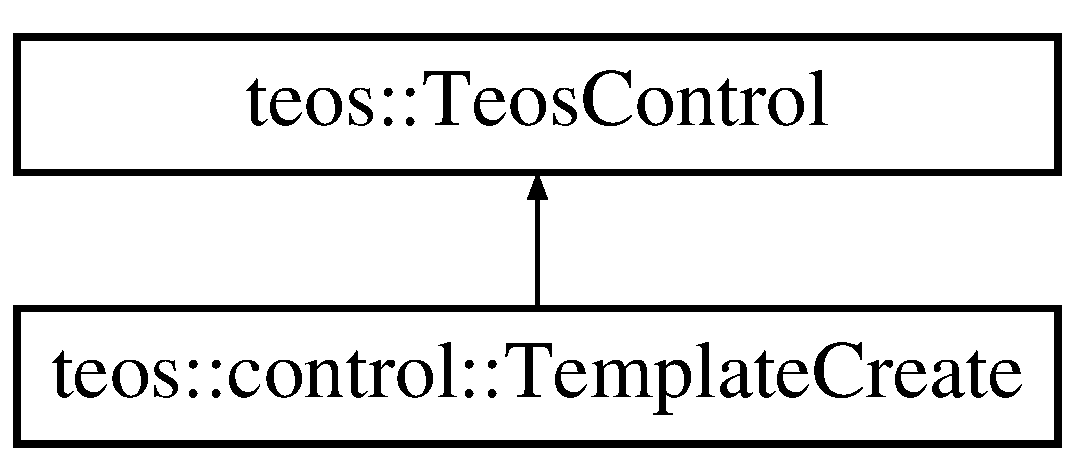
\includegraphics[height=2.000000cm]{classteos_1_1control_1_1_bootstrap_contract}
\end{center}
\end{figure}
\subsection*{Public Member Functions}
\begin{DoxyCompactItemize}
\item 
\mbox{\Hypertarget{classteos_1_1control_1_1_bootstrap_contract_a43979b7c9daa4406a374c18431e28407}\label{classteos_1_1control_1_1_bootstrap_contract_a43979b7c9daa4406a374c18431e28407}} 
{\bfseries Bootstrap\+Contract} (string name)
\item 
\mbox{\Hypertarget{classteos_1_1control_1_1_bootstrap_contract_ab7cbf4e4afab0d22739fbff222c1bd9e}\label{classteos_1_1control_1_1_bootstrap_contract_ab7cbf4e4afab0d22739fbff222c1bd9e}} 
{\bfseries Bootstrap\+Contract} (ptree req\+Json)
\end{DoxyCompactItemize}
\subsection*{Additional Inherited Members}


\subsection{Detailed Description}
\mbox{\hyperlink{classteos_1_1control_1_1_bootstrap_contract}{Bootstrap\+Contract}}\+: produces template contract workspace. 

The documentation for this class was generated from the following files\+:\begin{DoxyCompactItemize}
\item 
teos\+\_\+lib/include/teoslib/control/build\+\_\+contract.\+hpp\item 
teos\+\_\+lib/control/build\+\_\+contract.\+cpp\end{DoxyCompactItemize}

\hypertarget{classteos_1_1control_1_1_bootstrap_contract_options}{}\section{teos\+:\+:control\+:\+:Bootstrap\+Contract\+Options Class Reference}
\label{classteos_1_1control_1_1_bootstrap_contract_options}\index{teos\+::control\+::\+Bootstrap\+Contract\+Options@{teos\+::control\+::\+Bootstrap\+Contract\+Options}}


{\ttfamily \#include $<$build\+\_\+contract.\+hpp$>$}

Inheritance diagram for teos\+:\+:control\+:\+:Bootstrap\+Contract\+Options\+:\begin{figure}[H]
\begin{center}
\leavevmode
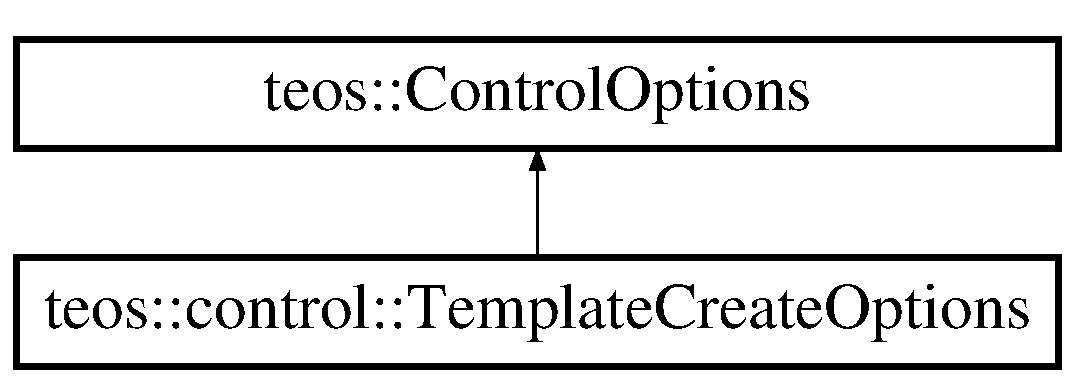
\includegraphics[height=2.000000cm]{classteos_1_1control_1_1_bootstrap_contract_options}
\end{center}
\end{figure}
\subsection*{Public Member Functions}
\begin{DoxyCompactItemize}
\item 
\mbox{\Hypertarget{classteos_1_1control_1_1_bootstrap_contract_options_aec7082f056fb85762b2fe0133481cd5f}\label{classteos_1_1control_1_1_bootstrap_contract_options_aec7082f056fb85762b2fe0133481cd5f}} 
{\bfseries Bootstrap\+Contract\+Options} (int argc, const char $\ast$$\ast$argv)
\end{DoxyCompactItemize}
\subsection*{Protected Member Functions}
\begin{DoxyCompactItemize}
\item 
const char $\ast$ \mbox{\hyperlink{classteos_1_1control_1_1_bootstrap_contract_options_af0f63b7aff6d7d41ac9b4b1c542b93f0}{get\+Usage}} ()
\begin{DoxyCompactList}\small\item\em Command \textquotesingle{}usage\textquotesingle{} instruction. \end{DoxyCompactList}\item 
\mbox{\Hypertarget{classteos_1_1control_1_1_bootstrap_contract_options_abb435f76b45d14ea9d26b6b4a94f4c0e}\label{classteos_1_1control_1_1_bootstrap_contract_options_abb435f76b45d14ea9d26b6b4a94f4c0e}} 
options\+\_\+description {\bfseries argument\+Description} ()
\item 
\mbox{\Hypertarget{classteos_1_1control_1_1_bootstrap_contract_options_a4658b45146d40cb330d0ca609fa1632e}\label{classteos_1_1control_1_1_bootstrap_contract_options_a4658b45146d40cb330d0ca609fa1632e}} 
void {\bfseries set\+Pos\+Desc} (positional\+\_\+options\+\_\+description \&pos\+\_\+desc)
\item 
\mbox{\Hypertarget{classteos_1_1control_1_1_bootstrap_contract_options_ae41d9ba25f072a5459e704b9f46c46b0}\label{classteos_1_1control_1_1_bootstrap_contract_options_ae41d9ba25f072a5459e704b9f46c46b0}} 
bool {\bfseries check\+Arguments} (variables\+\_\+map \&vm)
\item 
\mbox{\Hypertarget{classteos_1_1control_1_1_bootstrap_contract_options_a9f2bb15114542dcb293654e15c016df5}\label{classteos_1_1control_1_1_bootstrap_contract_options_a9f2bb15114542dcb293654e15c016df5}} 
\mbox{\hyperlink{classteos_1_1_teos_control}{Teos\+Control}} {\bfseries execute\+Command} ()
\item 
\mbox{\Hypertarget{classteos_1_1control_1_1_bootstrap_contract_options_afe65eb4b163e3d964177ac1312053a7a}\label{classteos_1_1control_1_1_bootstrap_contract_options_afe65eb4b163e3d964177ac1312053a7a}} 
void {\bfseries printout} (\mbox{\hyperlink{classteos_1_1_teos_control}{Teos\+Control}} command, variables\+\_\+map \&vm)
\end{DoxyCompactItemize}
\subsection*{Protected Attributes}
\begin{DoxyCompactItemize}
\item 
\mbox{\Hypertarget{classteos_1_1control_1_1_bootstrap_contract_options_ace24d9cab5c9188d816eb2253b68097f}\label{classteos_1_1control_1_1_bootstrap_contract_options_ace24d9cab5c9188d816eb2253b68097f}} 
string {\bfseries name}
\end{DoxyCompactItemize}


\subsection{Detailed Description}
Command-\/line driver for the \mbox{\hyperlink{classteos_1_1control_1_1_bootstrap_contract}{Bootstrap\+Contract}} class. 

\subsection{Member Function Documentation}
\mbox{\Hypertarget{classteos_1_1control_1_1_bootstrap_contract_options_af0f63b7aff6d7d41ac9b4b1c542b93f0}\label{classteos_1_1control_1_1_bootstrap_contract_options_af0f63b7aff6d7d41ac9b4b1c542b93f0}} 
\index{teos\+::control\+::\+Bootstrap\+Contract\+Options@{teos\+::control\+::\+Bootstrap\+Contract\+Options}!get\+Usage@{get\+Usage}}
\index{get\+Usage@{get\+Usage}!teos\+::control\+::\+Bootstrap\+Contract\+Options@{teos\+::control\+::\+Bootstrap\+Contract\+Options}}
\subsubsection{\texorpdfstring{get\+Usage()}{getUsage()}}
{\footnotesize\ttfamily const char$\ast$ teos\+::control\+::\+Bootstrap\+Contract\+Options\+::get\+Usage (\begin{DoxyParamCaption}{ }\end{DoxyParamCaption})\hspace{0.3cm}{\ttfamily [inline]}, {\ttfamily [protected]}, {\ttfamily [virtual]}}



Command \textquotesingle{}usage\textquotesingle{} instruction. 

\begin{DoxyReturn}{Returns}
usage text 
\end{DoxyReturn}


Reimplemented from \mbox{\hyperlink{classteos_1_1_control_options_a0aa5671f9bc750ed5280c26c543874f3}{teos\+::\+Control\+Options}}.



The documentation for this class was generated from the following file\+:\begin{DoxyCompactItemize}
\item 
include/teoslib/control/build\+\_\+contract.\+hpp\end{DoxyCompactItemize}

\hypertarget{classteos_1_1control_1_1_build_contract}{}\section{teos\+:\+:control\+:\+:Build\+Contract Class Reference}
\label{classteos_1_1control_1_1_build_contract}\index{teos\+::control\+::\+Build\+Contract@{teos\+::control\+::\+Build\+Contract}}


{\ttfamily \#include $<$build\+\_\+contract.\+hpp$>$}

Inheritance diagram for teos\+:\+:control\+:\+:Build\+Contract\+:\begin{figure}[H]
\begin{center}
\leavevmode
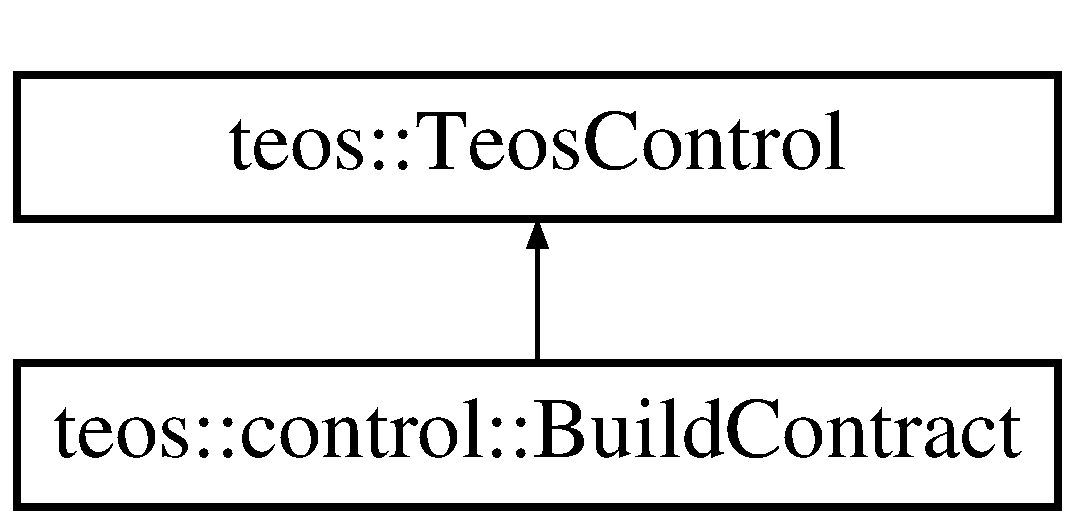
\includegraphics[height=2.000000cm]{classteos_1_1control_1_1_build_contract}
\end{center}
\end{figure}
\subsection*{Public Member Functions}
\begin{DoxyCompactItemize}
\item 
\mbox{\Hypertarget{classteos_1_1control_1_1_build_contract_a4e421b3614f96648b714a00610839f56}\label{classteos_1_1control_1_1_build_contract_a4e421b3614f96648b714a00610839f56}} 
{\bfseries Build\+Contract} (string src, string include\+\_\+dir=\char`\"{}\char`\"{})
\item 
\mbox{\Hypertarget{classteos_1_1control_1_1_build_contract_ac1bce2ea02bad0e31d3f7b9c06fef36e}\label{classteos_1_1control_1_1_build_contract_ac1bce2ea02bad0e31d3f7b9c06fef36e}} 
{\bfseries Build\+Contract} (ptree req\+Json)
\end{DoxyCompactItemize}
\subsection*{Additional Inherited Members}


\subsection{Detailed Description}
Builds a contract\+: produces the W\+A\+ST file. 

The documentation for this class was generated from the following files\+:\begin{DoxyCompactItemize}
\item 
include/teoslib/control/build\+\_\+contract.\+hpp\item 
control/build\+\_\+contract.\+cpp\end{DoxyCompactItemize}

\hypertarget{classteos_1_1control_1_1_build_contract_options}{}\section{teos\+:\+:control\+:\+:Build\+Contract\+Options Class Reference}
\label{classteos_1_1control_1_1_build_contract_options}\index{teos\+::control\+::\+Build\+Contract\+Options@{teos\+::control\+::\+Build\+Contract\+Options}}


{\ttfamily \#include $<$build\+\_\+contract.\+hpp$>$}

Inheritance diagram for teos\+:\+:control\+:\+:Build\+Contract\+Options\+:\begin{figure}[H]
\begin{center}
\leavevmode
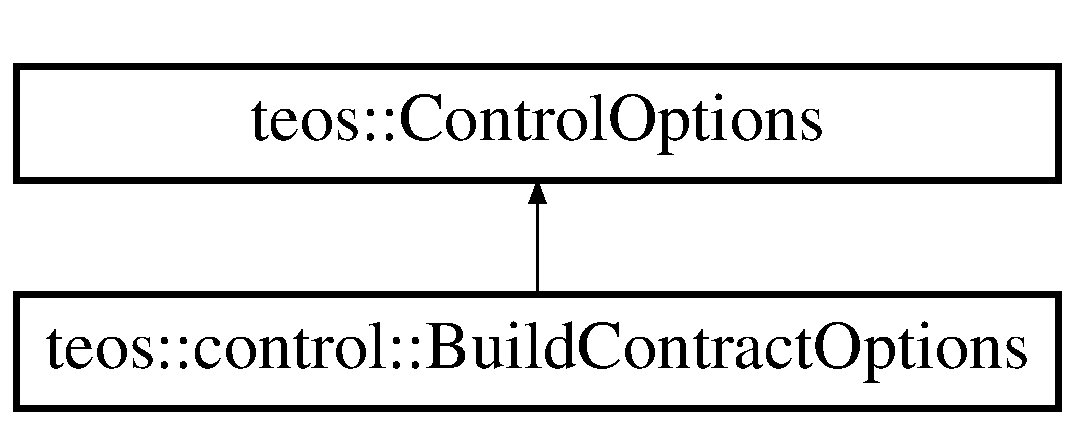
\includegraphics[height=2.000000cm]{classteos_1_1control_1_1_build_contract_options}
\end{center}
\end{figure}
\subsection*{Public Member Functions}
\begin{DoxyCompactItemize}
\item 
\mbox{\Hypertarget{classteos_1_1control_1_1_build_contract_options_a6d52cf1de31d636a9e823b46c7302834}\label{classteos_1_1control_1_1_build_contract_options_a6d52cf1de31d636a9e823b46c7302834}} 
{\bfseries Build\+Contract\+Options} (int argc, const char $\ast$$\ast$argv)
\end{DoxyCompactItemize}
\subsection*{Protected Member Functions}
\begin{DoxyCompactItemize}
\item 
const char $\ast$ \mbox{\hyperlink{classteos_1_1control_1_1_build_contract_options_ac45a323c2bc0c79b97b1d0d1d8afbf4f}{get\+Usage}} ()
\begin{DoxyCompactList}\small\item\em Command \textquotesingle{}usage\textquotesingle{} instruction. \end{DoxyCompactList}\item 
\mbox{\Hypertarget{classteos_1_1control_1_1_build_contract_options_abde356d5a17fa5fbcc4c8f777e4e537c}\label{classteos_1_1control_1_1_build_contract_options_abde356d5a17fa5fbcc4c8f777e4e537c}} 
options\+\_\+description {\bfseries argument\+Description} ()
\item 
\mbox{\Hypertarget{classteos_1_1control_1_1_build_contract_options_af43e12c147de6a8e890a8afd74bed117}\label{classteos_1_1control_1_1_build_contract_options_af43e12c147de6a8e890a8afd74bed117}} 
void {\bfseries set\+Pos\+Desc} (positional\+\_\+options\+\_\+description \&pos\+\_\+desc)
\item 
\mbox{\Hypertarget{classteos_1_1control_1_1_build_contract_options_a893d1aec857470781f69e478e5786b61}\label{classteos_1_1control_1_1_build_contract_options_a893d1aec857470781f69e478e5786b61}} 
bool {\bfseries check\+Arguments} (variables\+\_\+map \&vm)
\item 
\mbox{\Hypertarget{classteos_1_1control_1_1_build_contract_options_a2671a62aebae8e3cbe42ff94b9a92235}\label{classteos_1_1control_1_1_build_contract_options_a2671a62aebae8e3cbe42ff94b9a92235}} 
\mbox{\hyperlink{classteos_1_1_teos_control}{Teos\+Control}} {\bfseries execute\+Command} ()
\item 
\mbox{\Hypertarget{classteos_1_1control_1_1_build_contract_options_a01e81d8723fb8f9c8f12c13c5cf70c7f}\label{classteos_1_1control_1_1_build_contract_options_a01e81d8723fb8f9c8f12c13c5cf70c7f}} 
void {\bfseries printout} (\mbox{\hyperlink{classteos_1_1_teos_control}{Teos\+Control}} command, variables\+\_\+map \&vm)
\end{DoxyCompactItemize}
\subsection*{Protected Attributes}
\begin{DoxyCompactItemize}
\item 
\mbox{\Hypertarget{classteos_1_1control_1_1_build_contract_options_a80b02b6769efd16a94bc83e7991dc7db}\label{classteos_1_1control_1_1_build_contract_options_a80b02b6769efd16a94bc83e7991dc7db}} 
string {\bfseries src}
\item 
\mbox{\Hypertarget{classteos_1_1control_1_1_build_contract_options_ae9784fdf0854b5ee6d9e9b2edf0b0345}\label{classteos_1_1control_1_1_build_contract_options_ae9784fdf0854b5ee6d9e9b2edf0b0345}} 
string {\bfseries wast\+\_\+file}
\item 
\mbox{\Hypertarget{classteos_1_1control_1_1_build_contract_options_a4e5b55589b7062925301c383f5bb8bab}\label{classteos_1_1control_1_1_build_contract_options_a4e5b55589b7062925301c383f5bb8bab}} 
string {\bfseries include\+\_\+dir}
\item 
\mbox{\Hypertarget{classteos_1_1control_1_1_build_contract_options_a6a92e41ed58131c1358f9f9a9b69b71a}\label{classteos_1_1control_1_1_build_contract_options_a6a92e41ed58131c1358f9f9a9b69b71a}} 
bool {\bfseries compile\+\_\+only}
\end{DoxyCompactItemize}


\subsection{Detailed Description}
Command-\/line driver for the \mbox{\hyperlink{classteos_1_1control_1_1_build_contract}{Build\+Contract}} class. 

\subsection{Member Function Documentation}
\mbox{\Hypertarget{classteos_1_1control_1_1_build_contract_options_ac45a323c2bc0c79b97b1d0d1d8afbf4f}\label{classteos_1_1control_1_1_build_contract_options_ac45a323c2bc0c79b97b1d0d1d8afbf4f}} 
\index{teos\+::control\+::\+Build\+Contract\+Options@{teos\+::control\+::\+Build\+Contract\+Options}!get\+Usage@{get\+Usage}}
\index{get\+Usage@{get\+Usage}!teos\+::control\+::\+Build\+Contract\+Options@{teos\+::control\+::\+Build\+Contract\+Options}}
\subsubsection{\texorpdfstring{get\+Usage()}{getUsage()}}
{\footnotesize\ttfamily const char$\ast$ teos\+::control\+::\+Build\+Contract\+Options\+::get\+Usage (\begin{DoxyParamCaption}{ }\end{DoxyParamCaption})\hspace{0.3cm}{\ttfamily [inline]}, {\ttfamily [protected]}, {\ttfamily [virtual]}}



Command \textquotesingle{}usage\textquotesingle{} instruction. 

\begin{DoxyReturn}{Returns}
usage text 
\end{DoxyReturn}


Reimplemented from \mbox{\hyperlink{classteos_1_1_control_options_a0aa5671f9bc750ed5280c26c543874f3}{teos\+::\+Control\+Options}}.



The documentation for this class was generated from the following file\+:\begin{DoxyCompactItemize}
\item 
teos\+\_\+lib/include/teoslib/control/build\+\_\+contract.\+hpp\end{DoxyCompactItemize}

\hypertarget{classteos_1_1command_1_1_call_chain}{}\section{teos\+:\+:command\+:\+:Call\+Chain Class Reference}
\label{classteos_1_1command_1_1_call_chain}\index{teos\+::command\+::\+Call\+Chain@{teos\+::command\+::\+Call\+Chain}}
Inheritance diagram for teos\+:\+:command\+:\+:Call\+Chain\+:\begin{figure}[H]
\begin{center}
\leavevmode
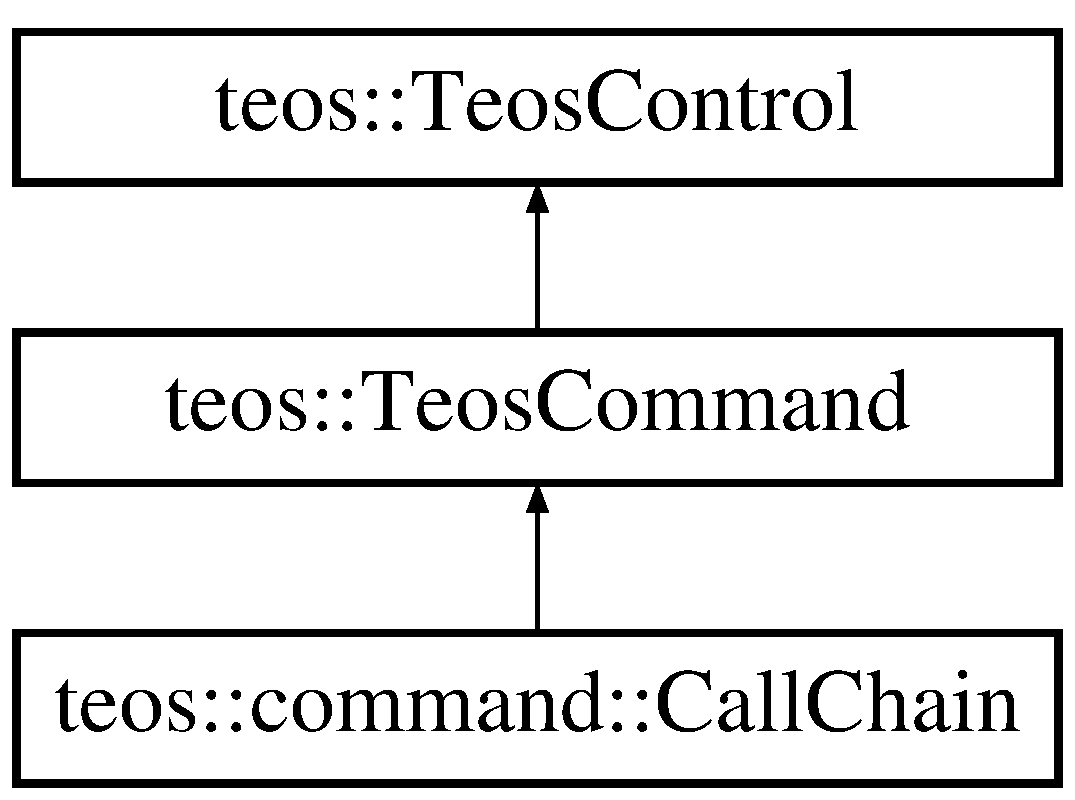
\includegraphics[height=3.000000cm]{classteos_1_1command_1_1_call_chain}
\end{center}
\end{figure}
\subsection*{Public Member Functions}
\begin{DoxyCompactItemize}
\item 
\mbox{\Hypertarget{classteos_1_1command_1_1_call_chain_a040b1c9a31e3a73890c6e3a4b19e98f7}\label{classteos_1_1command_1_1_call_chain_a040b1c9a31e3a73890c6e3a4b19e98f7}} 
bool {\bfseries fca\+Variant2ptree} (const fc\+::variant \&post\+Data, ptree \&json)
\item 
\mbox{\Hypertarget{classteos_1_1command_1_1_call_chain_a9f7d8b56d513bd808666e1d46ec624a5}\label{classteos_1_1command_1_1_call_chain_a9f7d8b56d513bd808666e1d46ec624a5}} 
{\bfseries Call\+Chain} (string path, const fc\+::variant \&post\+Data=fc\+::variant())
\item 
\mbox{\Hypertarget{classteos_1_1command_1_1_call_chain_ac7d7a03c159c1e5970bc16339bd0c25f}\label{classteos_1_1command_1_1_call_chain_ac7d7a03c159c1e5970bc16339bd0c25f}} 
{\bfseries Call\+Chain} (fc\+::variant fc\+Variant)
\item 
\mbox{\Hypertarget{classteos_1_1command_1_1_call_chain_a967cd6e68b60916f23b6c9651f4238a5}\label{classteos_1_1command_1_1_call_chain_a967cd6e68b60916f23b6c9651f4238a5}} 
std\+::string {\bfseries norm\+Request} (ptree \&reg\+Json)
\item 
\mbox{\Hypertarget{classteos_1_1command_1_1_call_chain_ac98ff4043a6ee0f8b9d3e2e4467f4988}\label{classteos_1_1command_1_1_call_chain_ac98ff4043a6ee0f8b9d3e2e4467f4988}} 
void {\bfseries norm\+Response} (std\+::string response, ptree \&resp\+Json)
\end{DoxyCompactItemize}
\subsection*{Public Attributes}
\begin{DoxyCompactItemize}
\item 
\mbox{\Hypertarget{classteos_1_1command_1_1_call_chain_a0afbe899ce8a5039702701e82f7ec9f2}\label{classteos_1_1command_1_1_call_chain_a0afbe899ce8a5039702701e82f7ec9f2}} 
fc\+::variant {\bfseries fc\+Variant\+\_\+}
\end{DoxyCompactItemize}
\subsection*{Additional Inherited Members}


The documentation for this class was generated from the following file\+:\begin{DoxyCompactItemize}
\item 
eos\+\_\+interface.\+cpp\end{DoxyCompactItemize}

\hypertarget{classteos_1_1_command_options}{}\section{teos\+:\+:Command\+Options Class Reference}
\label{classteos_1_1_command_options}\index{teos\+::\+Command\+Options@{teos\+::\+Command\+Options}}
Inheritance diagram for teos\+:\+:Command\+Options\+:\begin{figure}[H]
\begin{center}
\leavevmode
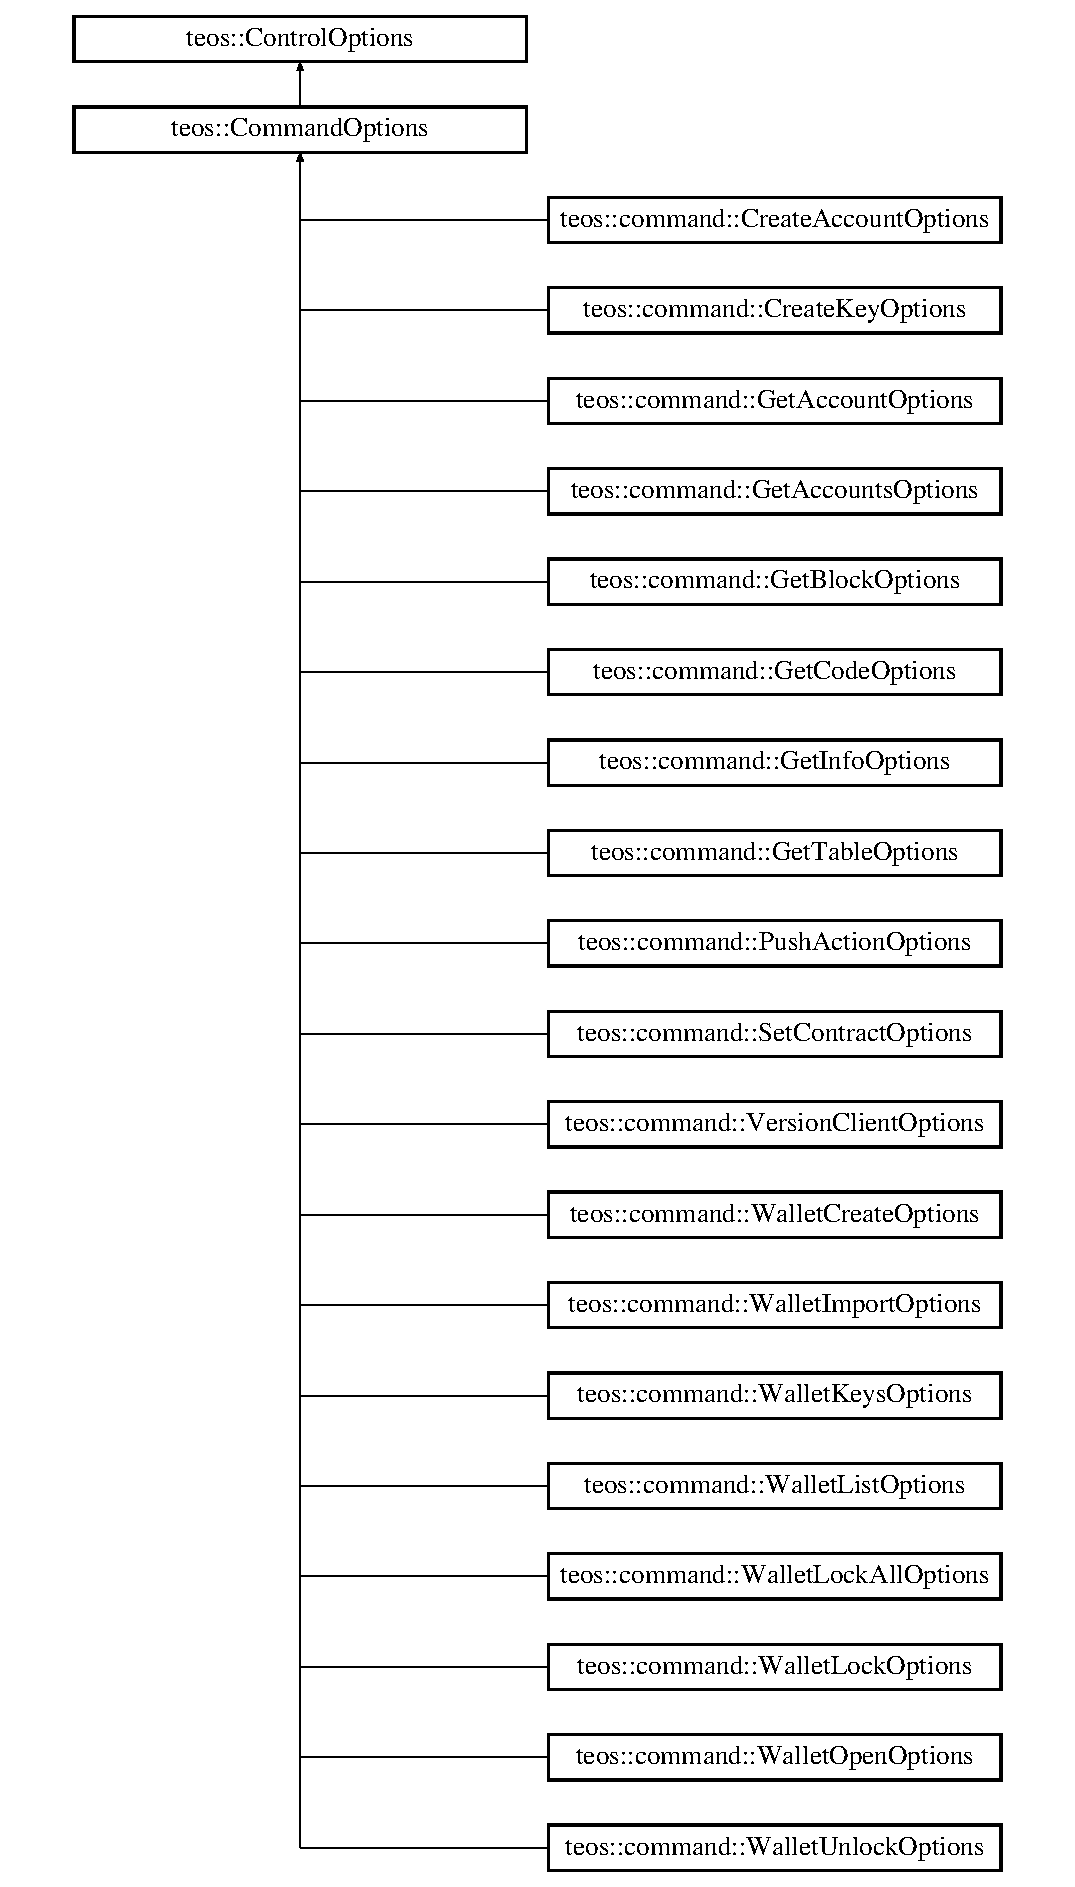
\includegraphics[height=12.000000cm]{classteos_1_1_command_options}
\end{center}
\end{figure}
\subsection*{Public Member Functions}
\begin{DoxyCompactItemize}
\item 
\mbox{\Hypertarget{classteos_1_1_command_options_aa0fc4c9930fe2bf479abdbe187a4ca65}\label{classteos_1_1_command_options_aa0fc4c9930fe2bf479abdbe187a4ca65}} 
{\bfseries Command\+Options} (int argc, const char $\ast$argv\mbox{[}$\,$\mbox{]})
\end{DoxyCompactItemize}
\subsection*{Static Public Member Functions}
\begin{DoxyCompactItemize}
\item 
\mbox{\Hypertarget{classteos_1_1_command_options_a64481990f4f43f58491bb5def15006c5}\label{classteos_1_1_command_options_a64481990f4f43f58491bb5def15006c5}} 
static options\+\_\+description {\bfseries http\+Options} ()
\end{DoxyCompactItemize}
\subsection*{Protected Member Functions}
\begin{DoxyCompactItemize}
\item 
\mbox{\Hypertarget{classteos_1_1_command_options_ad9cb8c834296b2c5dee2a82c006bfa0c}\label{classteos_1_1_command_options_ad9cb8c834296b2c5dee2a82c006bfa0c}} 
options\+\_\+description {\bfseries group\+Option\+Description} ()
\end{DoxyCompactItemize}
\subsection*{Additional Inherited Members}


The documentation for this class was generated from the following file\+:\begin{DoxyCompactItemize}
\item 
teos\+\_\+lib/include/teoslib/\mbox{\hyperlink{command_8hpp}{command.\+hpp}}\end{DoxyCompactItemize}

\hypertarget{classteos_1_1_control_options}{}\section{teos\+:\+:Control\+Options Class Reference}
\label{classteos_1_1_control_options}\index{teos\+::\+Control\+Options@{teos\+::\+Control\+Options}}
Inheritance diagram for teos\+:\+:Control\+Options\+:\begin{figure}[H]
\begin{center}
\leavevmode
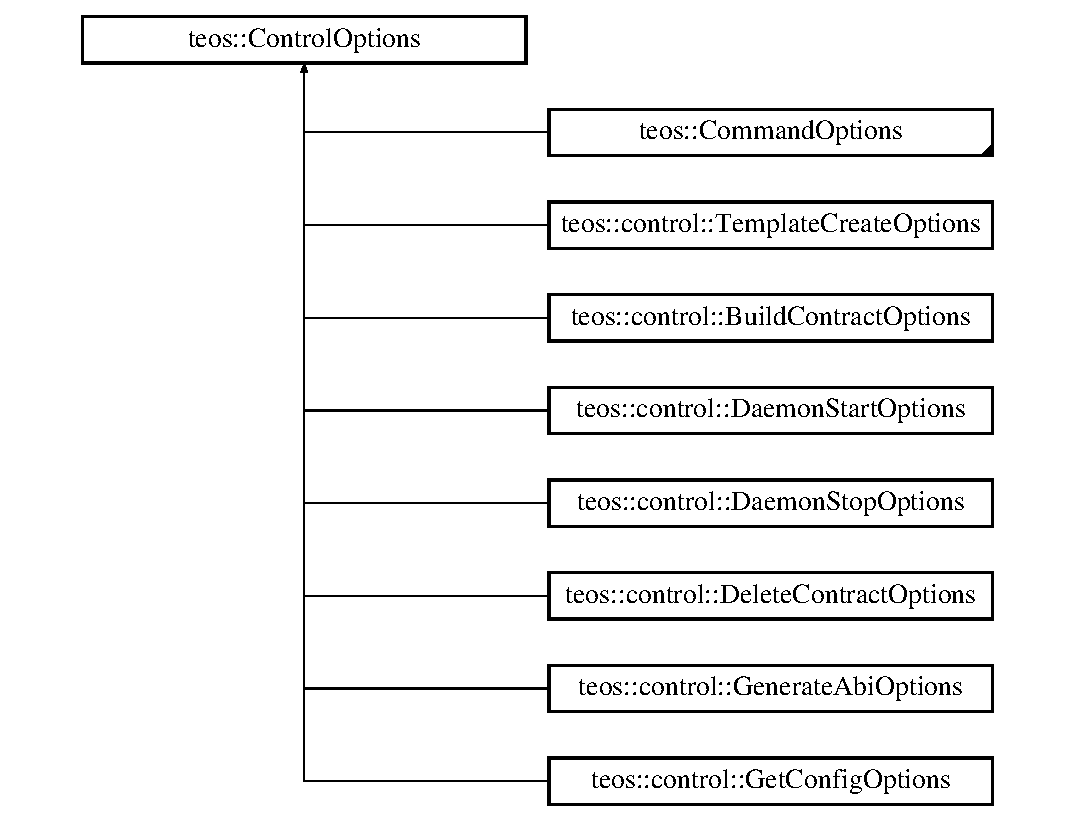
\includegraphics[height=9.000000cm]{classteos_1_1_control_options}
\end{center}
\end{figure}
\subsection*{Public Member Functions}
\begin{DoxyCompactItemize}
\item 
\mbox{\Hypertarget{classteos_1_1_control_options_ae997028704fe0f8086096d7fa4b71ee9}\label{classteos_1_1_control_options_ae997028704fe0f8086096d7fa4b71ee9}} 
{\bfseries Control\+Options} (int argc, const char $\ast$argv\mbox{[}$\,$\mbox{]})
\item 
\mbox{\Hypertarget{classteos_1_1_control_options_ad3496976524c0ca5288018725119fb39}\label{classteos_1_1_control_options_ad3496976524c0ca5288018725119fb39}} 
void {\bfseries go} ()
\end{DoxyCompactItemize}
\subsection*{Protected Member Functions}
\begin{DoxyCompactItemize}
\item 
\mbox{\Hypertarget{classteos_1_1_control_options_a490f2d5ea05e92a5996beaa6d40c5c32}\label{classteos_1_1_control_options_a490f2d5ea05e92a5996beaa6d40c5c32}} 
options\+\_\+description {\bfseries basic\+Option\+Description} ()
\item 
\mbox{\Hypertarget{classteos_1_1_control_options_a611508b33386c2a2465e68b333b51c5f}\label{classteos_1_1_control_options_a611508b33386c2a2465e68b333b51c5f}} 
virtual options\+\_\+description {\bfseries argument\+Description} ()
\item 
\mbox{\Hypertarget{classteos_1_1_control_options_a1b39c9263e1abea919db8097b46ecfae}\label{classteos_1_1_control_options_a1b39c9263e1abea919db8097b46ecfae}} 
virtual options\+\_\+description {\bfseries group\+Option\+Description} ()
\item 
virtual const char $\ast$ \mbox{\hyperlink{classteos_1_1_control_options_a0aa5671f9bc750ed5280c26c543874f3}{get\+Usage}} ()
\begin{DoxyCompactList}\small\item\em Command \textquotesingle{}usage\textquotesingle{} instruction. \end{DoxyCompactList}\item 
\mbox{\Hypertarget{classteos_1_1_control_options_a606085ad334d59eafc103be85e3be146}\label{classteos_1_1_control_options_a606085ad334d59eafc103be85e3be146}} 
virtual void {\bfseries set\+Pos\+Desc} (positional\+\_\+options\+\_\+description \&pos\+\_\+descr)
\item 
\mbox{\Hypertarget{classteos_1_1_control_options_a33001fdd58dea6056f683a8e280c245e}\label{classteos_1_1_control_options_a33001fdd58dea6056f683a8e280c245e}} 
virtual void {\bfseries printout} (\mbox{\hyperlink{classteos_1_1_teos_control}{Teos\+Control}} command, variables\+\_\+map \&vm)
\item 
\mbox{\Hypertarget{classteos_1_1_control_options_a2916fdad936906cec8496b5952936cae}\label{classteos_1_1_control_options_a2916fdad936906cec8496b5952936cae}} 
virtual bool {\bfseries check\+Arguments} (variables\+\_\+map \&vm)
\item 
\mbox{\Hypertarget{classteos_1_1_control_options_a46025212b1afd9b9e56914844512ac24}\label{classteos_1_1_control_options_a46025212b1afd9b9e56914844512ac24}} 
virtual void {\bfseries parse\+Group\+Variables\+Map} (variables\+\_\+map \&vm)
\item 
\mbox{\Hypertarget{classteos_1_1_control_options_afc04b2ed27c6b2497a95890498d403d0}\label{classteos_1_1_control_options_afc04b2ed27c6b2497a95890498d403d0}} 
virtual \mbox{\hyperlink{classteos_1_1_teos_control}{Teos\+Control}} {\bfseries execute\+Command} ()
\end{DoxyCompactItemize}
\subsection*{Protected Attributes}
\begin{DoxyCompactItemize}
\item 
\mbox{\Hypertarget{classteos_1_1_control_options_a385705bd05cf4cc33892f51737585f9b}\label{classteos_1_1_control_options_a385705bd05cf4cc33892f51737585f9b}} 
string {\bfseries json\+\_\+}
\item 
\mbox{\Hypertarget{classteos_1_1_control_options_aef27b07fd43f5e553f20138deb57657a}\label{classteos_1_1_control_options_aef27b07fd43f5e553f20138deb57657a}} 
ptree {\bfseries req\+Json\+\_\+}
\end{DoxyCompactItemize}


\subsection{Member Function Documentation}
\mbox{\Hypertarget{classteos_1_1_control_options_a0aa5671f9bc750ed5280c26c543874f3}\label{classteos_1_1_control_options_a0aa5671f9bc750ed5280c26c543874f3}} 
\index{teos\+::\+Control\+Options@{teos\+::\+Control\+Options}!get\+Usage@{get\+Usage}}
\index{get\+Usage@{get\+Usage}!teos\+::\+Control\+Options@{teos\+::\+Control\+Options}}
\subsubsection{\texorpdfstring{get\+Usage()}{getUsage()}}
{\footnotesize\ttfamily virtual const char$\ast$ teos\+::\+Control\+Options\+::get\+Usage (\begin{DoxyParamCaption}{ }\end{DoxyParamCaption})\hspace{0.3cm}{\ttfamily [inline]}, {\ttfamily [protected]}, {\ttfamily [virtual]}}



Command \textquotesingle{}usage\textquotesingle{} instruction. 

\begin{DoxyReturn}{Returns}
usage text 
\end{DoxyReturn}


Reimplemented in \mbox{\hyperlink{classteos_1_1command_1_1_wallet_keys_options_a40097f0265580b2c3cdaad721f5cef09}{teos\+::command\+::\+Wallet\+Keys\+Options}}, \mbox{\hyperlink{classteos_1_1command_1_1_wallet_unlock_options_aa630c4deec62ef8d44cb37c03573c071}{teos\+::command\+::\+Wallet\+Unlock\+Options}}, \mbox{\hyperlink{classteos_1_1command_1_1_wallet_lock_all_options_ae45881c064f3d14883f3a1fae105603a}{teos\+::command\+::\+Wallet\+Lock\+All\+Options}}, \mbox{\hyperlink{classteos_1_1command_1_1_get_table_options_a764b61a7d83e508673b73100c45c3d13}{teos\+::command\+::\+Get\+Table\+Options}}, \mbox{\hyperlink{classteos_1_1command_1_1_wallet_lock_options_aa0b3fd6dc244e1f32955c7a134b4fd85}{teos\+::command\+::\+Wallet\+Lock\+Options}}, \mbox{\hyperlink{classteos_1_1command_1_1_get_code_options_a62a3c2c3cc72eb8b9bd5034fb335c7e2}{teos\+::command\+::\+Get\+Code\+Options}}, \mbox{\hyperlink{classteos_1_1control_1_1_delete_contract_options_abca9a6e25e4bcaf14b130199f32e4fbf}{teos\+::control\+::\+Delete\+Contract\+Options}}, \mbox{\hyperlink{classteos_1_1command_1_1_wallet_open_options_aedf25a6f772392c2cb0c0de8d80172dd}{teos\+::command\+::\+Wallet\+Open\+Options}}, \mbox{\hyperlink{classteos_1_1command_1_1_create_key_options_ac4c7176d534ed832ebfc954e36238a4c}{teos\+::command\+::\+Create\+Key\+Options}}, \mbox{\hyperlink{classteos_1_1command_1_1_get_accounts_options_ac93b806fa601124aa899474da62d1288}{teos\+::command\+::\+Get\+Accounts\+Options}}, \mbox{\hyperlink{classteos_1_1control_1_1_bootstrap_contract_options_af0f63b7aff6d7d41ac9b4b1c542b93f0}{teos\+::control\+::\+Bootstrap\+Contract\+Options}}, \mbox{\hyperlink{classteos_1_1command_1_1_wallet_list_options_ae6394f5f8c311fc9e56b0d44562cea67}{teos\+::command\+::\+Wallet\+List\+Options}}, \mbox{\hyperlink{classteos_1_1command_1_1_get_account_options_a987381bcf3f687b7babfe197edf0dc26}{teos\+::command\+::\+Get\+Account\+Options}}, \mbox{\hyperlink{classteos_1_1command_1_1_wallet_import_options_ad641b37bd61f2d4ff3e3049e2dd6be0e}{teos\+::command\+::\+Wallet\+Import\+Options}}, \mbox{\hyperlink{classteos_1_1control_1_1_generate_abi_options_a7d2ce1ad86518ee06e0bc5ffbe104b39}{teos\+::control\+::\+Generate\+Abi\+Options}}, \mbox{\hyperlink{classteos_1_1command_1_1_get_block_options_a85970d4f6337e594d2ac0756f67c50f7}{teos\+::command\+::\+Get\+Block\+Options}}, \mbox{\hyperlink{classteos_1_1command_1_1_create_account_options_af5c13799a676966824e5e9e47b1af180}{teos\+::command\+::\+Create\+Account\+Options}}, \mbox{\hyperlink{classteos_1_1control_1_1_daemon_start_options_ae036aeede350023308b66b063ba00bd8}{teos\+::control\+::\+Daemon\+Start\+Options}}, \mbox{\hyperlink{classteos_1_1command_1_1_set_contract_options_a9176e2b58b222d45c975d6e9fa9b4ac7}{teos\+::command\+::\+Set\+Contract\+Options}}, \mbox{\hyperlink{classteos_1_1command_1_1_push_action_options_a1dac78e7b40cc0ff91895d1fc0f7d2b4}{teos\+::command\+::\+Push\+Action\+Options}}, \mbox{\hyperlink{classteos_1_1command_1_1_wallet_create_options_ad20c1955cb48f6c9e640c35eae091c30}{teos\+::command\+::\+Wallet\+Create\+Options}}, \mbox{\hyperlink{classteos_1_1control_1_1_get_config_options_a144b88309b989f2282da43ad56ddb1a6}{teos\+::control\+::\+Get\+Config\+Options}}, \mbox{\hyperlink{classteos_1_1command_1_1_get_info_options_af5b6ec0a42f019ef1058e6f78a84346d}{teos\+::command\+::\+Get\+Info\+Options}}, \mbox{\hyperlink{classteos_1_1control_1_1_build_contract_options_ac45a323c2bc0c79b97b1d0d1d8afbf4f}{teos\+::control\+::\+Build\+Contract\+Options}}, \mbox{\hyperlink{classteos_1_1command_1_1_version_client_options_a28b69107e8eb50a2faf9594958bb1d6d}{teos\+::command\+::\+Version\+Client\+Options}}, and \mbox{\hyperlink{classteos_1_1control_1_1_daemon_stop_options_a99e7d5a47cd20e4ad437049263cd367a}{teos\+::control\+::\+Daemon\+Stop\+Options}}.



The documentation for this class was generated from the following file\+:\begin{DoxyCompactItemize}
\item 
include/teoslib/control.\+hpp\end{DoxyCompactItemize}

\hypertarget{classteos_1_1command_1_1_create_account}{}\section{teos\+:\+:command\+:\+:Create\+Account Class Reference}
\label{classteos_1_1command_1_1_create_account}\index{teos\+::command\+::\+Create\+Account@{teos\+::command\+::\+Create\+Account}}


{\ttfamily \#include $<$create\+\_\+commands.\+hpp$>$}

Inheritance diagram for teos\+:\+:command\+:\+:Create\+Account\+:\begin{figure}[H]
\begin{center}
\leavevmode
\includegraphics[height=4.000000cm]{classteos_1_1command_1_1_create_account}
\end{center}
\end{figure}
\subsection*{Public Member Functions}
\begin{DoxyCompactItemize}
\item 
\mbox{\Hypertarget{classteos_1_1command_1_1_create_account_aa5fc119e457ddaa39bb04d94c95430c2}\label{classteos_1_1command_1_1_create_account_aa5fc119e457ddaa39bb04d94c95430c2}} 
{\bfseries Create\+Account} (string creator, string account\+Name, string owner\+Key\+Publ, string active\+Key\+Publ, string permission=\char`\"{}\char`\"{}, unsigned expiration\+Sec=30, bool skip\+Signature=false, bool dont\+Broadcast=false, bool force\+Unique=false, unsigned max\+Cpu\+Usage=0, unsigned max\+Net\+Usage=0)
\item 
\mbox{\Hypertarget{classteos_1_1command_1_1_create_account_a5431fb149148b10c14e59b4fc0e99fbd}\label{classteos_1_1command_1_1_create_account_a5431fb149148b10c14e59b4fc0e99fbd}} 
{\bfseries Create\+Account} (ptree req\+Json)
\end{DoxyCompactItemize}
\subsection*{Additional Inherited Members}


\subsection{Detailed Description}
Creates a new account on the blockchain. 

The documentation for this class was generated from the following file\+:\begin{DoxyCompactItemize}
\item 
include/teoslib/command/create\+\_\+commands.\+hpp\end{DoxyCompactItemize}

\hypertarget{classteos_1_1command_1_1_create_account_options}{}\section{teos\+:\+:command\+:\+:Create\+Account\+Options Class Reference}
\label{classteos_1_1command_1_1_create_account_options}\index{teos\+::command\+::\+Create\+Account\+Options@{teos\+::command\+::\+Create\+Account\+Options}}


Command-\/line driver for the \mbox{\hyperlink{classteos_1_1command_1_1_create_account}{Create\+Account}} class.  




{\ttfamily \#include $<$create\+\_\+commands.\+hpp$>$}

Inheritance diagram for teos\+:\+:command\+:\+:Create\+Account\+Options\+:\begin{figure}[H]
\begin{center}
\leavevmode
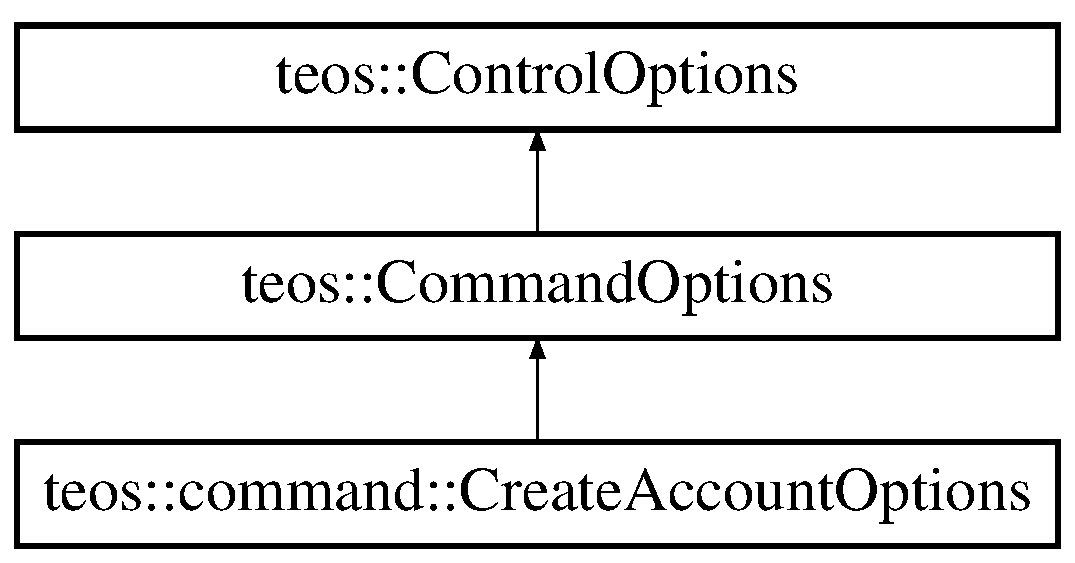
\includegraphics[height=3.000000cm]{classteos_1_1command_1_1_create_account_options}
\end{center}
\end{figure}
\subsection*{Public Member Functions}
\begin{DoxyCompactItemize}
\item 
\mbox{\Hypertarget{classteos_1_1command_1_1_create_account_options_a885bd48ad537054b0541bcc82e2848c7}\label{classteos_1_1command_1_1_create_account_options_a885bd48ad537054b0541bcc82e2848c7}} 
{\bfseries Create\+Account\+Options} (int argc, const char $\ast$$\ast$argv)
\end{DoxyCompactItemize}
\subsection*{Protected Member Functions}
\begin{DoxyCompactItemize}
\item 
\mbox{\Hypertarget{classteos_1_1command_1_1_create_account_options_ae755f847b91be57be448f6ed3a8b8009}\label{classteos_1_1command_1_1_create_account_options_ae755f847b91be57be448f6ed3a8b8009}} 
string {\bfseries get\+Transaction\+Usage} ()
\item 
const char $\ast$ \mbox{\hyperlink{classteos_1_1command_1_1_create_account_options_af5c13799a676966824e5e9e47b1af180}{get\+Usage}} ()
\begin{DoxyCompactList}\small\item\em Command \textquotesingle{}usage\textquotesingle{} instruction. \end{DoxyCompactList}\item 
\mbox{\Hypertarget{classteos_1_1command_1_1_create_account_options_aaaa292c801f19000ed073ca752a34ce2}\label{classteos_1_1command_1_1_create_account_options_aaaa292c801f19000ed073ca752a34ce2}} 
options\+\_\+description {\bfseries transaction\+Options} ()
\item 
\mbox{\Hypertarget{classteos_1_1command_1_1_create_account_options_aed8f14bd484aaecff46a27f1dd1288cd}\label{classteos_1_1command_1_1_create_account_options_aed8f14bd484aaecff46a27f1dd1288cd}} 
options\+\_\+description {\bfseries argument\+Description} ()
\item 
\mbox{\Hypertarget{classteos_1_1command_1_1_create_account_options_a892d104e8131e44a8420f8aca3a590a3}\label{classteos_1_1command_1_1_create_account_options_a892d104e8131e44a8420f8aca3a590a3}} 
void {\bfseries set\+Pos\+Desc} (positional\+\_\+options\+\_\+description \&pos\+\_\+desc)
\item 
\mbox{\Hypertarget{classteos_1_1command_1_1_create_account_options_af5aab64759b629ccdc261f4e3f434a3e}\label{classteos_1_1command_1_1_create_account_options_af5aab64759b629ccdc261f4e3f434a3e}} 
void {\bfseries transaction\+Args} ()
\item 
\mbox{\Hypertarget{classteos_1_1command_1_1_create_account_options_a481f9c6206512f1afc8bc6729f8dc76b}\label{classteos_1_1command_1_1_create_account_options_a481f9c6206512f1afc8bc6729f8dc76b}} 
bool {\bfseries check\+Arguments} (variables\+\_\+map \&vm)
\item 
\mbox{\Hypertarget{classteos_1_1command_1_1_create_account_options_a60ecaec7f5e305ee8c97844cbcdda197}\label{classteos_1_1command_1_1_create_account_options_a60ecaec7f5e305ee8c97844cbcdda197}} 
\mbox{\hyperlink{classteos_1_1_teos_control}{Teos\+Control}} {\bfseries execute\+Command} ()
\item 
\mbox{\Hypertarget{classteos_1_1command_1_1_create_account_options_a2f4f089db5a69624545292ad2243bc11}\label{classteos_1_1command_1_1_create_account_options_a2f4f089db5a69624545292ad2243bc11}} 
void {\bfseries printout} (\mbox{\hyperlink{classteos_1_1_teos_control}{Teos\+Control}} command, variables\+\_\+map \&vm)
\end{DoxyCompactItemize}
\subsection*{Protected Attributes}
\begin{DoxyCompactItemize}
\item 
\mbox{\Hypertarget{classteos_1_1command_1_1_create_account_options_a242584daf28306388158a4be3cc599d2}\label{classteos_1_1command_1_1_create_account_options_a242584daf28306388158a4be3cc599d2}} 
string {\bfseries permission}
\item 
\mbox{\Hypertarget{classteos_1_1command_1_1_create_account_options_a3c047b24f9efe02637569d2d944ad0dc}\label{classteos_1_1command_1_1_create_account_options_a3c047b24f9efe02637569d2d944ad0dc}} 
unsigned {\bfseries expiration}
\item 
\mbox{\Hypertarget{classteos_1_1command_1_1_create_account_options_a99e99fe49e9f88ac06d8e0f52e9c2ea5}\label{classteos_1_1command_1_1_create_account_options_a99e99fe49e9f88ac06d8e0f52e9c2ea5}} 
bool {\bfseries skip\+Signature}
\item 
\mbox{\Hypertarget{classteos_1_1command_1_1_create_account_options_a0f017486e409d3037355d0a164a2e4e0}\label{classteos_1_1command_1_1_create_account_options_a0f017486e409d3037355d0a164a2e4e0}} 
bool {\bfseries dont\+Broadcast}
\item 
\mbox{\Hypertarget{classteos_1_1command_1_1_create_account_options_adb4da4cc70268eaa54414bf1c73ee604}\label{classteos_1_1command_1_1_create_account_options_adb4da4cc70268eaa54414bf1c73ee604}} 
bool {\bfseries force\+Unique}
\item 
\mbox{\Hypertarget{classteos_1_1command_1_1_create_account_options_adb934651202adf807e9722de99727501}\label{classteos_1_1command_1_1_create_account_options_adb934651202adf807e9722de99727501}} 
unsigned {\bfseries max\+Cpu\+Usage}
\item 
\mbox{\Hypertarget{classteos_1_1command_1_1_create_account_options_a24c6ed3d29a86fb662abed2e46568477}\label{classteos_1_1command_1_1_create_account_options_a24c6ed3d29a86fb662abed2e46568477}} 
unsigned {\bfseries max\+Net\+Usage}
\item 
\mbox{\Hypertarget{classteos_1_1command_1_1_create_account_options_af9576b1dac22ecac291ac0b850dd33e1}\label{classteos_1_1command_1_1_create_account_options_af9576b1dac22ecac291ac0b850dd33e1}} 
string {\bfseries creator}
\item 
\mbox{\Hypertarget{classteos_1_1command_1_1_create_account_options_a3eb4bc50ad5681004a3e50250cab96f2}\label{classteos_1_1command_1_1_create_account_options_a3eb4bc50ad5681004a3e50250cab96f2}} 
string {\bfseries name}
\item 
\mbox{\Hypertarget{classteos_1_1command_1_1_create_account_options_a87425103161912ddcf3ff2cc8b477273}\label{classteos_1_1command_1_1_create_account_options_a87425103161912ddcf3ff2cc8b477273}} 
string {\bfseries owner\+Key}
\item 
\mbox{\Hypertarget{classteos_1_1command_1_1_create_account_options_a9a68bb2c9e028001b47ad880a8f2ec0b}\label{classteos_1_1command_1_1_create_account_options_a9a68bb2c9e028001b47ad880a8f2ec0b}} 
string {\bfseries active\+Key}
\end{DoxyCompactItemize}
\subsection*{Additional Inherited Members}


\subsection{Detailed Description}
Command-\/line driver for the \mbox{\hyperlink{classteos_1_1command_1_1_create_account}{Create\+Account}} class. 

\subsection{Member Function Documentation}
\mbox{\Hypertarget{classteos_1_1command_1_1_create_account_options_af5c13799a676966824e5e9e47b1af180}\label{classteos_1_1command_1_1_create_account_options_af5c13799a676966824e5e9e47b1af180}} 
\index{teos\+::command\+::\+Create\+Account\+Options@{teos\+::command\+::\+Create\+Account\+Options}!get\+Usage@{get\+Usage}}
\index{get\+Usage@{get\+Usage}!teos\+::command\+::\+Create\+Account\+Options@{teos\+::command\+::\+Create\+Account\+Options}}
\subsubsection{\texorpdfstring{get\+Usage()}{getUsage()}}
{\footnotesize\ttfamily const char$\ast$ teos\+::command\+::\+Create\+Account\+Options\+::get\+Usage (\begin{DoxyParamCaption}{ }\end{DoxyParamCaption})\hspace{0.3cm}{\ttfamily [inline]}, {\ttfamily [protected]}, {\ttfamily [virtual]}}



Command \textquotesingle{}usage\textquotesingle{} instruction. 

\begin{DoxyReturn}{Returns}
usage text 
\end{DoxyReturn}


Reimplemented from \mbox{\hyperlink{classteos_1_1_control_options_a0aa5671f9bc750ed5280c26c543874f3}{teos\+::\+Control\+Options}}.



The documentation for this class was generated from the following file\+:\begin{DoxyCompactItemize}
\item 
teos\+\_\+lib/include/teoslib/command/create\+\_\+commands.\+hpp\end{DoxyCompactItemize}

\hypertarget{classteos_1_1command_1_1_create_key}{}\section{teos\+:\+:command\+:\+:Create\+Key Class Reference}
\label{classteos_1_1command_1_1_create_key}\index{teos\+::command\+::\+Create\+Key@{teos\+::command\+::\+Create\+Key}}


Create a new keypair and print the public and private keys.  




{\ttfamily \#include $<$create\+\_\+commands.\+hpp$>$}

Inheritance diagram for teos\+:\+:command\+:\+:Create\+Key\+:\begin{figure}[H]
\begin{center}
\leavevmode
\includegraphics[height=4.000000cm]{classteos_1_1command_1_1_create_key}
\end{center}
\end{figure}
\subsection*{Public Member Functions}
\begin{DoxyCompactItemize}
\item 
\mbox{\hyperlink{classteos_1_1command_1_1_create_key_a9908b3b01b818ccd742978a0b74c9745}{Create\+Key}} (string key\+Name)
\begin{DoxyCompactList}\small\item\em A constructor. \end{DoxyCompactList}\item 
\mbox{\hyperlink{classteos_1_1command_1_1_create_key_a9e09786f8c0cef5e37d041567627e9fd}{Create\+Key}} (ptree req\+Json)
\begin{DoxyCompactList}\small\item\em A constructor. \end{DoxyCompactList}\end{DoxyCompactItemize}
\subsection*{Additional Inherited Members}


\subsection{Detailed Description}
Create a new keypair and print the public and private keys. 

\subsection{Constructor \& Destructor Documentation}
\mbox{\Hypertarget{classteos_1_1command_1_1_create_key_a9908b3b01b818ccd742978a0b74c9745}\label{classteos_1_1command_1_1_create_key_a9908b3b01b818ccd742978a0b74c9745}} 
\index{teos\+::command\+::\+Create\+Key@{teos\+::command\+::\+Create\+Key}!Create\+Key@{Create\+Key}}
\index{Create\+Key@{Create\+Key}!teos\+::command\+::\+Create\+Key@{teos\+::command\+::\+Create\+Key}}
\subsubsection{\texorpdfstring{Create\+Key()}{CreateKey()}\hspace{0.1cm}{\footnotesize\ttfamily [1/2]}}
{\footnotesize\ttfamily teos\+::command\+::\+Create\+Key\+::\+Create\+Key (\begin{DoxyParamCaption}\item[{string}]{key\+Name }\end{DoxyParamCaption})\hspace{0.3cm}{\ttfamily [inline]}}



A constructor. 


\begin{DoxyParams}{Parameters}
{\em key\+Name} & key-\/pair id. \char`\"{}private\+Key\char`\"{}\+:\char`\"{}$<$private key$>$\char`\"{} \char`\"{}public\+Key\char`\"{}\+:\char`\"{}$<$public key$>$\char`\"{}\}. \\
\hline
\end{DoxyParams}
\mbox{\Hypertarget{classteos_1_1command_1_1_create_key_a9e09786f8c0cef5e37d041567627e9fd}\label{classteos_1_1command_1_1_create_key_a9e09786f8c0cef5e37d041567627e9fd}} 
\index{teos\+::command\+::\+Create\+Key@{teos\+::command\+::\+Create\+Key}!Create\+Key@{Create\+Key}}
\index{Create\+Key@{Create\+Key}!teos\+::command\+::\+Create\+Key@{teos\+::command\+::\+Create\+Key}}
\subsubsection{\texorpdfstring{Create\+Key()}{CreateKey()}\hspace{0.1cm}{\footnotesize\ttfamily [2/2]}}
{\footnotesize\ttfamily teos\+::command\+::\+Create\+Key\+::\+Create\+Key (\begin{DoxyParamCaption}\item[{ptree}]{req\+Json }\end{DoxyParamCaption})\hspace{0.3cm}{\ttfamily [inline]}}



A constructor. 


\begin{DoxyParams}{Parameters}
{\em req\+Json} & a boost json tree argument\+: \{\char`\"{}key\+Name\char`\"{}\+:\char`\"{}$<$key name$>$\char`\"{}\}. \char`\"{}private\+Key\char`\"{}\+:\char`\"{}$<$private key$>$\char`\"{} \char`\"{}public\+Key\char`\"{}\+:\char`\"{}$<$public key$>$\char`\"{}\}. \\
\hline
\end{DoxyParams}


The documentation for this class was generated from the following file\+:\begin{DoxyCompactItemize}
\item 
teos\+\_\+lib/include/teoslib/command/create\+\_\+commands.\+hpp\end{DoxyCompactItemize}

\hypertarget{classteos_1_1command_1_1_create_key_options}{}\section{teos\+:\+:command\+:\+:Create\+Key\+Options Class Reference}
\label{classteos_1_1command_1_1_create_key_options}\index{teos\+::command\+::\+Create\+Key\+Options@{teos\+::command\+::\+Create\+Key\+Options}}


Command-\/line driver for the \mbox{\hyperlink{classteos_1_1command_1_1_create_key}{Create\+Key}} class.  




{\ttfamily \#include $<$create\+\_\+commands.\+hpp$>$}

Inheritance diagram for teos\+:\+:command\+:\+:Create\+Key\+Options\+:\begin{figure}[H]
\begin{center}
\leavevmode
\includegraphics[height=3.000000cm]{classteos_1_1command_1_1_create_key_options}
\end{center}
\end{figure}
\subsection*{Public Member Functions}
\begin{DoxyCompactItemize}
\item 
\mbox{\Hypertarget{classteos_1_1command_1_1_create_key_options_afc955f866552d0f24ce9e09423b98778}\label{classteos_1_1command_1_1_create_key_options_afc955f866552d0f24ce9e09423b98778}} 
{\bfseries Create\+Key\+Options} (int argc, const char $\ast$$\ast$argv)
\end{DoxyCompactItemize}
\subsection*{Protected Member Functions}
\begin{DoxyCompactItemize}
\item 
const char $\ast$ \mbox{\hyperlink{classteos_1_1command_1_1_create_key_options_ac4c7176d534ed832ebfc954e36238a4c}{get\+Usage}} ()
\begin{DoxyCompactList}\small\item\em Command \textquotesingle{}usage\textquotesingle{} instruction. \end{DoxyCompactList}\item 
\mbox{\Hypertarget{classteos_1_1command_1_1_create_key_options_ad05b210e6e7f9930ed7438ab21257a34}\label{classteos_1_1command_1_1_create_key_options_ad05b210e6e7f9930ed7438ab21257a34}} 
options\+\_\+description {\bfseries argument\+Description} ()
\item 
\mbox{\Hypertarget{classteos_1_1command_1_1_create_key_options_aaead04dd480db9516e8ccdfd4533b949}\label{classteos_1_1command_1_1_create_key_options_aaead04dd480db9516e8ccdfd4533b949}} 
void {\bfseries set\+Pos\+Desc} (positional\+\_\+options\+\_\+description \&pos\+\_\+desc)
\item 
\mbox{\Hypertarget{classteos_1_1command_1_1_create_key_options_a46cc7933de9c2a71c111bdcfd9a327a8}\label{classteos_1_1command_1_1_create_key_options_a46cc7933de9c2a71c111bdcfd9a327a8}} 
bool {\bfseries check\+Arguments} (variables\+\_\+map \&vm)
\item 
\mbox{\Hypertarget{classteos_1_1command_1_1_create_key_options_af47c20b59e773febdfb5f1e2ed0ea735}\label{classteos_1_1command_1_1_create_key_options_af47c20b59e773febdfb5f1e2ed0ea735}} 
\mbox{\hyperlink{classteos_1_1_teos_control}{Teos\+Control}} {\bfseries execute\+Command} ()
\item 
\mbox{\Hypertarget{classteos_1_1command_1_1_create_key_options_a94087926f6ea43b7c05d57f86ae8995b}\label{classteos_1_1command_1_1_create_key_options_a94087926f6ea43b7c05d57f86ae8995b}} 
void {\bfseries printout} (\mbox{\hyperlink{classteos_1_1_teos_control}{Teos\+Control}} command, variables\+\_\+map \&vm)
\end{DoxyCompactItemize}
\subsection*{Protected Attributes}
\begin{DoxyCompactItemize}
\item 
\mbox{\Hypertarget{classteos_1_1command_1_1_create_key_options_a0e908701e5d4f6a5583ef1fdd244da37}\label{classteos_1_1command_1_1_create_key_options_a0e908701e5d4f6a5583ef1fdd244da37}} 
string {\bfseries key\+Name}
\end{DoxyCompactItemize}
\subsection*{Additional Inherited Members}


\subsection{Detailed Description}
Command-\/line driver for the \mbox{\hyperlink{classteos_1_1command_1_1_create_key}{Create\+Key}} class. 

\subsection{Member Function Documentation}
\mbox{\Hypertarget{classteos_1_1command_1_1_create_key_options_ac4c7176d534ed832ebfc954e36238a4c}\label{classteos_1_1command_1_1_create_key_options_ac4c7176d534ed832ebfc954e36238a4c}} 
\index{teos\+::command\+::\+Create\+Key\+Options@{teos\+::command\+::\+Create\+Key\+Options}!get\+Usage@{get\+Usage}}
\index{get\+Usage@{get\+Usage}!teos\+::command\+::\+Create\+Key\+Options@{teos\+::command\+::\+Create\+Key\+Options}}
\subsubsection{\texorpdfstring{get\+Usage()}{getUsage()}}
{\footnotesize\ttfamily const char$\ast$ teos\+::command\+::\+Create\+Key\+Options\+::get\+Usage (\begin{DoxyParamCaption}{ }\end{DoxyParamCaption})\hspace{0.3cm}{\ttfamily [inline]}, {\ttfamily [protected]}, {\ttfamily [virtual]}}



Command \textquotesingle{}usage\textquotesingle{} instruction. 

\begin{DoxyReturn}{Returns}
usage text 
\end{DoxyReturn}


Reimplemented from \mbox{\hyperlink{classteos_1_1_control_options_a0aa5671f9bc750ed5280c26c543874f3}{teos\+::\+Control\+Options}}.



The documentation for this class was generated from the following file\+:\begin{DoxyCompactItemize}
\item 
include/teoslib/command/create\+\_\+commands.\+hpp\end{DoxyCompactItemize}

\hypertarget{classteos_1_1control_1_1_daemon_start}{}\section{teos\+:\+:control\+:\+:Daemon\+Start Class Reference}
\label{classteos_1_1control_1_1_daemon_start}\index{teos\+::control\+::\+Daemon\+Start@{teos\+::control\+::\+Daemon\+Start}}


Start a test E\+O\+S\+IO daemon if no one is running.  




{\ttfamily \#include $<$daemon\+\_\+controls.\+hpp$>$}

Inheritance diagram for teos\+:\+:control\+:\+:Daemon\+Start\+:\begin{figure}[H]
\begin{center}
\leavevmode
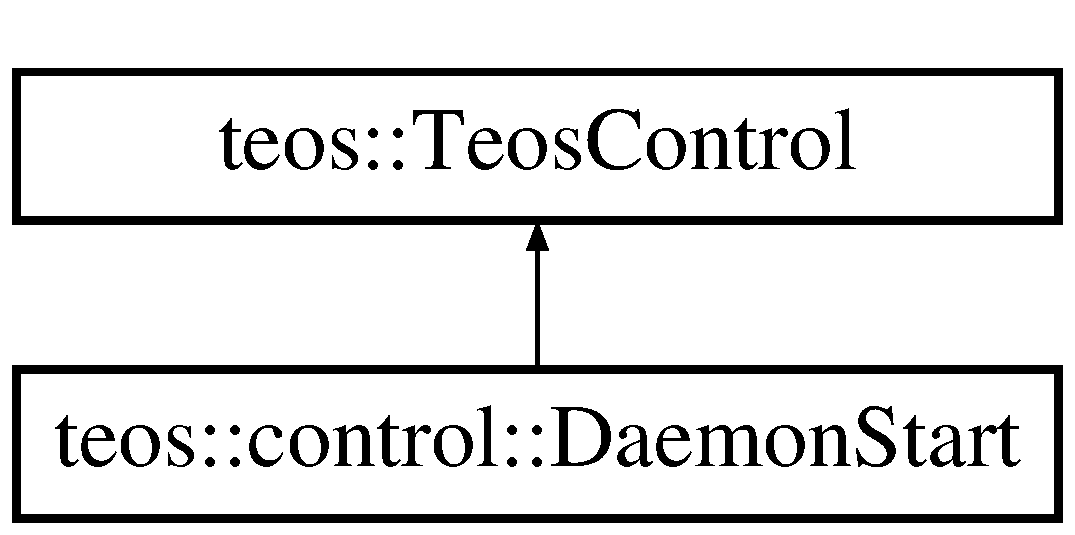
\includegraphics[height=2.000000cm]{classteos_1_1control_1_1_daemon_start}
\end{center}
\end{figure}
\subsection*{Public Member Functions}
\begin{DoxyCompactItemize}
\item 
\mbox{\Hypertarget{classteos_1_1control_1_1_daemon_start_a5a17511cf7eabb346b645f3c34ebfb63}\label{classteos_1_1control_1_1_daemon_start_a5a17511cf7eabb346b645f3c34ebfb63}} 
{\bfseries Daemon\+Start} (bool resync\+\_\+blockchain=false)
\item 
\mbox{\Hypertarget{classteos_1_1control_1_1_daemon_start_ae6f2b43eaab462ec4683c9f56ec35019}\label{classteos_1_1control_1_1_daemon_start_ae6f2b43eaab462ec4683c9f56ec35019}} 
{\bfseries Daemon\+Start} (ptree req\+Json)
\end{DoxyCompactItemize}
\subsection*{Static Public Attributes}
\begin{DoxyCompactItemize}
\item 
\mbox{\Hypertarget{classteos_1_1control_1_1_daemon_start_ad63b0523ef8e608be7d6c22694763f00}\label{classteos_1_1control_1_1_daemon_start_ad63b0523ef8e608be7d6c22694763f00}} 
static const string {\bfseries D\+O\+\_\+\+N\+O\+T\+\_\+\+L\+A\+U\+N\+CH} = \char`\"{}D\+O\+\_\+\+N\+O\+T\+\_\+\+L\+A\+U\+N\+CH\char`\"{}
\end{DoxyCompactItemize}
\subsection*{Additional Inherited Members}


\subsection{Detailed Description}
Start a test E\+O\+S\+IO daemon if no one is running. 

The documentation for this class was generated from the following files\+:\begin{DoxyCompactItemize}
\item 
include/teoslib/control/daemon\+\_\+controls.\+hpp\item 
control/daemon\+\_\+controls.\+cpp\end{DoxyCompactItemize}

\hypertarget{classteos_1_1control_1_1_daemon_start_options}{}\section{teos\+:\+:control\+:\+:Daemon\+Start\+Options Class Reference}
\label{classteos_1_1control_1_1_daemon_start_options}\index{teos\+::control\+::\+Daemon\+Start\+Options@{teos\+::control\+::\+Daemon\+Start\+Options}}
Inheritance diagram for teos\+:\+:control\+:\+:Daemon\+Start\+Options\+:\begin{figure}[H]
\begin{center}
\leavevmode
\includegraphics[height=2.000000cm]{classteos_1_1control_1_1_daemon_start_options}
\end{center}
\end{figure}
\subsection*{Public Member Functions}
\begin{DoxyCompactItemize}
\item 
\mbox{\Hypertarget{classteos_1_1control_1_1_daemon_start_options_ad5c4bad7dbec78a18444db1be27b7b2b}\label{classteos_1_1control_1_1_daemon_start_options_ad5c4bad7dbec78a18444db1be27b7b2b}} 
{\bfseries Daemon\+Start\+Options} (int argc, const char $\ast$$\ast$argv)
\end{DoxyCompactItemize}
\subsection*{Protected Member Functions}
\begin{DoxyCompactItemize}
\item 
const char $\ast$ \mbox{\hyperlink{classteos_1_1control_1_1_daemon_start_options_ae036aeede350023308b66b063ba00bd8}{get\+Usage}} ()
\begin{DoxyCompactList}\small\item\em Command \textquotesingle{}usage\textquotesingle{} instruction. \end{DoxyCompactList}\item 
\mbox{\Hypertarget{classteos_1_1control_1_1_daemon_start_options_ab3960fbf33433037a08ef46e0baeedb7}\label{classteos_1_1control_1_1_daemon_start_options_ab3960fbf33433037a08ef46e0baeedb7}} 
options\+\_\+description {\bfseries argument\+Description} ()
\item 
\mbox{\Hypertarget{classteos_1_1control_1_1_daemon_start_options_a51c828308709fb55cfdde2af4443e976}\label{classteos_1_1control_1_1_daemon_start_options_a51c828308709fb55cfdde2af4443e976}} 
bool {\bfseries check\+Arguments} (variables\+\_\+map \&vm)
\item 
\mbox{\Hypertarget{classteos_1_1control_1_1_daemon_start_options_ab02fafd8670769f90b749ba60baf6708}\label{classteos_1_1control_1_1_daemon_start_options_ab02fafd8670769f90b749ba60baf6708}} 
\mbox{\hyperlink{classteos_1_1_teos_control}{Teos\+Control}} {\bfseries execute\+Command} ()
\item 
\mbox{\Hypertarget{classteos_1_1control_1_1_daemon_start_options_a2dda2e522e76c941e540737cf1149151}\label{classteos_1_1control_1_1_daemon_start_options_a2dda2e522e76c941e540737cf1149151}} 
void {\bfseries printout} (\mbox{\hyperlink{classteos_1_1_teos_control}{Teos\+Control}} command, variables\+\_\+map \&vm)
\end{DoxyCompactItemize}
\subsection*{Additional Inherited Members}


\subsection{Member Function Documentation}
\mbox{\Hypertarget{classteos_1_1control_1_1_daemon_start_options_ae036aeede350023308b66b063ba00bd8}\label{classteos_1_1control_1_1_daemon_start_options_ae036aeede350023308b66b063ba00bd8}} 
\index{teos\+::control\+::\+Daemon\+Start\+Options@{teos\+::control\+::\+Daemon\+Start\+Options}!get\+Usage@{get\+Usage}}
\index{get\+Usage@{get\+Usage}!teos\+::control\+::\+Daemon\+Start\+Options@{teos\+::control\+::\+Daemon\+Start\+Options}}
\subsubsection{\texorpdfstring{get\+Usage()}{getUsage()}}
{\footnotesize\ttfamily const char$\ast$ teos\+::control\+::\+Daemon\+Start\+Options\+::get\+Usage (\begin{DoxyParamCaption}{ }\end{DoxyParamCaption})\hspace{0.3cm}{\ttfamily [inline]}, {\ttfamily [protected]}, {\ttfamily [virtual]}}



Command \textquotesingle{}usage\textquotesingle{} instruction. 

\begin{DoxyReturn}{Returns}
usage text 
\end{DoxyReturn}


Reimplemented from \mbox{\hyperlink{classteos_1_1_control_options_a0aa5671f9bc750ed5280c26c543874f3}{teos\+::\+Control\+Options}}.



The documentation for this class was generated from the following file\+:\begin{DoxyCompactItemize}
\item 
include/teoslib/control/daemon\+\_\+controls.\+hpp\end{DoxyCompactItemize}

\hypertarget{classteos_1_1control_1_1_daemon_stop}{}\section{teos\+:\+:control\+:\+:Daemon\+Stop Class Reference}
\label{classteos_1_1control_1_1_daemon_stop}\index{teos\+::control\+::\+Daemon\+Stop@{teos\+::control\+::\+Daemon\+Stop}}


Kill a running E\+OS node process.  




{\ttfamily \#include $<$daemon\+\_\+controls.\+hpp$>$}

Inheritance diagram for teos\+:\+:control\+:\+:Daemon\+Stop\+:\begin{figure}[H]
\begin{center}
\leavevmode
\includegraphics[height=2.000000cm]{classteos_1_1control_1_1_daemon_stop}
\end{center}
\end{figure}
\subsection*{Additional Inherited Members}


\subsection{Detailed Description}
Kill a running E\+OS node process. 

The documentation for this class was generated from the following files\+:\begin{DoxyCompactItemize}
\item 
teos\+\_\+lib/include/teoslib/control/daemon\+\_\+controls.\+hpp\item 
teos\+\_\+lib/control/daemon\+\_\+controls.\+cpp\end{DoxyCompactItemize}

\hypertarget{classteos_1_1control_1_1_daemon_stop_options}{}\section{teos\+:\+:control\+:\+:Daemon\+Stop\+Options Class Reference}
\label{classteos_1_1control_1_1_daemon_stop_options}\index{teos\+::control\+::\+Daemon\+Stop\+Options@{teos\+::control\+::\+Daemon\+Stop\+Options}}
Inheritance diagram for teos\+:\+:control\+:\+:Daemon\+Stop\+Options\+:\begin{figure}[H]
\begin{center}
\leavevmode
\includegraphics[height=2.000000cm]{classteos_1_1control_1_1_daemon_stop_options}
\end{center}
\end{figure}
\subsection*{Public Member Functions}
\begin{DoxyCompactItemize}
\item 
\mbox{\Hypertarget{classteos_1_1control_1_1_daemon_stop_options_a518c6d0d85866b13aae28500da7637bb}\label{classteos_1_1control_1_1_daemon_stop_options_a518c6d0d85866b13aae28500da7637bb}} 
{\bfseries Daemon\+Stop\+Options} (int argc, const char $\ast$$\ast$argv)
\end{DoxyCompactItemize}
\subsection*{Protected Member Functions}
\begin{DoxyCompactItemize}
\item 
const char $\ast$ \mbox{\hyperlink{classteos_1_1control_1_1_daemon_stop_options_a99e7d5a47cd20e4ad437049263cd367a}{get\+Usage}} ()
\begin{DoxyCompactList}\small\item\em Command \textquotesingle{}usage\textquotesingle{} instruction. \end{DoxyCompactList}\item 
\mbox{\Hypertarget{classteos_1_1control_1_1_daemon_stop_options_afb91935bea6f426383c3b88d035fe03c}\label{classteos_1_1control_1_1_daemon_stop_options_afb91935bea6f426383c3b88d035fe03c}} 
\mbox{\hyperlink{classteos_1_1_teos_control}{Teos\+Control}} {\bfseries execute\+Command} ()
\item 
\mbox{\Hypertarget{classteos_1_1control_1_1_daemon_stop_options_af7e6dac1e8dfd8750f8101e6b48b4912}\label{classteos_1_1control_1_1_daemon_stop_options_af7e6dac1e8dfd8750f8101e6b48b4912}} 
void {\bfseries printout} (\mbox{\hyperlink{classteos_1_1_teos_control}{Teos\+Control}} command, variables\+\_\+map \&vm)
\end{DoxyCompactItemize}
\subsection*{Additional Inherited Members}


\subsection{Member Function Documentation}
\mbox{\Hypertarget{classteos_1_1control_1_1_daemon_stop_options_a99e7d5a47cd20e4ad437049263cd367a}\label{classteos_1_1control_1_1_daemon_stop_options_a99e7d5a47cd20e4ad437049263cd367a}} 
\index{teos\+::control\+::\+Daemon\+Stop\+Options@{teos\+::control\+::\+Daemon\+Stop\+Options}!get\+Usage@{get\+Usage}}
\index{get\+Usage@{get\+Usage}!teos\+::control\+::\+Daemon\+Stop\+Options@{teos\+::control\+::\+Daemon\+Stop\+Options}}
\subsubsection{\texorpdfstring{get\+Usage()}{getUsage()}}
{\footnotesize\ttfamily const char$\ast$ teos\+::control\+::\+Daemon\+Stop\+Options\+::get\+Usage (\begin{DoxyParamCaption}{ }\end{DoxyParamCaption})\hspace{0.3cm}{\ttfamily [inline]}, {\ttfamily [protected]}, {\ttfamily [virtual]}}



Command \textquotesingle{}usage\textquotesingle{} instruction. 

\begin{DoxyReturn}{Returns}
usage text 
\end{DoxyReturn}


Reimplemented from \mbox{\hyperlink{classteos_1_1_control_options_a0aa5671f9bc750ed5280c26c543874f3}{teos\+::\+Control\+Options}}.



The documentation for this class was generated from the following file\+:\begin{DoxyCompactItemize}
\item 
teos\+\_\+lib/include/teoslib/control/daemon\+\_\+controls.\+hpp\end{DoxyCompactItemize}

\hypertarget{classteos_1_1control_1_1_delete_contract}{}\section{teos\+:\+:control\+:\+:Delete\+Contract Class Reference}
\label{classteos_1_1control_1_1_delete_contract}\index{teos\+::control\+::\+Delete\+Contract@{teos\+::control\+::\+Delete\+Contract}}


{\ttfamily \#include $<$build\+\_\+contract.\+hpp$>$}

Inheritance diagram for teos\+:\+:control\+:\+:Delete\+Contract\+:\begin{figure}[H]
\begin{center}
\leavevmode
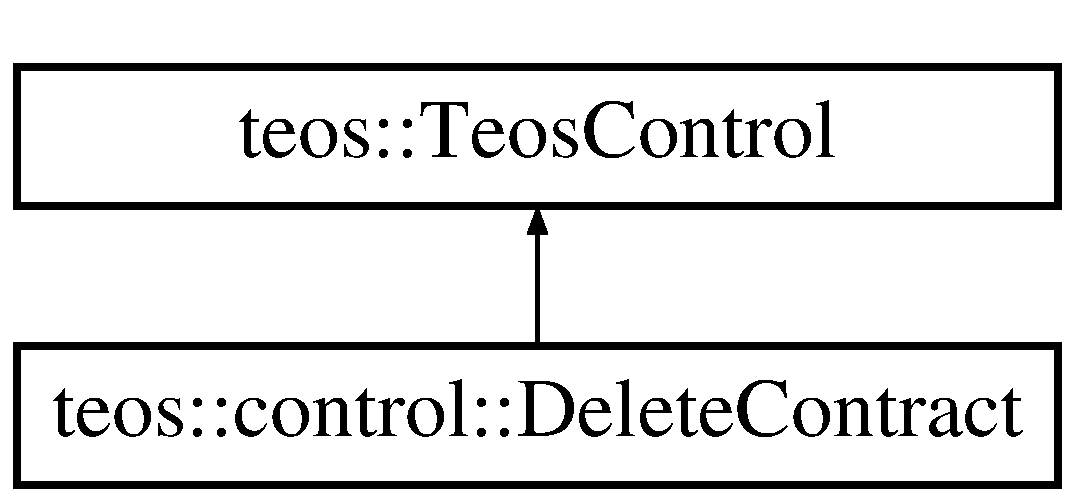
\includegraphics[height=2.000000cm]{classteos_1_1control_1_1_delete_contract}
\end{center}
\end{figure}
\subsection*{Public Member Functions}
\begin{DoxyCompactItemize}
\item 
\mbox{\Hypertarget{classteos_1_1control_1_1_delete_contract_a9f91d7395f390ff68db2417d73be8c35}\label{classteos_1_1control_1_1_delete_contract_a9f91d7395f390ff68db2417d73be8c35}} 
{\bfseries Delete\+Contract} (string name)
\item 
\mbox{\Hypertarget{classteos_1_1control_1_1_delete_contract_ac519ac86917200febf0195a4d2ce60ab}\label{classteos_1_1control_1_1_delete_contract_ac519ac86917200febf0195a4d2ce60ab}} 
{\bfseries Delete\+Contract} (ptree req\+Json)
\end{DoxyCompactItemize}
\subsection*{Additional Inherited Members}


\subsection{Detailed Description}
\mbox{\hyperlink{classteos_1_1control_1_1_bootstrap_contract}{Bootstrap\+Contract}}\+: produces template contract workspace. 

The documentation for this class was generated from the following files\+:\begin{DoxyCompactItemize}
\item 
teos\+\_\+lib/include/teoslib/control/build\+\_\+contract.\+hpp\item 
teos\+\_\+lib/control/build\+\_\+contract.\+cpp\end{DoxyCompactItemize}

\hypertarget{classteos_1_1control_1_1_delete_contract_options}{}\section{teos\+:\+:control\+:\+:Delete\+Contract\+Options Class Reference}
\label{classteos_1_1control_1_1_delete_contract_options}\index{teos\+::control\+::\+Delete\+Contract\+Options@{teos\+::control\+::\+Delete\+Contract\+Options}}


{\ttfamily \#include $<$build\+\_\+contract.\+hpp$>$}

Inheritance diagram for teos\+:\+:control\+:\+:Delete\+Contract\+Options\+:\begin{figure}[H]
\begin{center}
\leavevmode
\includegraphics[height=2.000000cm]{classteos_1_1control_1_1_delete_contract_options}
\end{center}
\end{figure}
\subsection*{Public Member Functions}
\begin{DoxyCompactItemize}
\item 
\mbox{\Hypertarget{classteos_1_1control_1_1_delete_contract_options_afc38af8415d9ab6117a00fb21437f903}\label{classteos_1_1control_1_1_delete_contract_options_afc38af8415d9ab6117a00fb21437f903}} 
{\bfseries Delete\+Contract\+Options} (int argc, const char $\ast$$\ast$argv)
\end{DoxyCompactItemize}
\subsection*{Protected Member Functions}
\begin{DoxyCompactItemize}
\item 
const char $\ast$ \mbox{\hyperlink{classteos_1_1control_1_1_delete_contract_options_abca9a6e25e4bcaf14b130199f32e4fbf}{get\+Usage}} ()
\begin{DoxyCompactList}\small\item\em Command \textquotesingle{}usage\textquotesingle{} instruction. \end{DoxyCompactList}\item 
\mbox{\Hypertarget{classteos_1_1control_1_1_delete_contract_options_a96771a4727132887b02f77e25a8e99e3}\label{classteos_1_1control_1_1_delete_contract_options_a96771a4727132887b02f77e25a8e99e3}} 
options\+\_\+description {\bfseries argument\+Description} ()
\item 
\mbox{\Hypertarget{classteos_1_1control_1_1_delete_contract_options_ad2f35a525326b954a3a88f93aabbed67}\label{classteos_1_1control_1_1_delete_contract_options_ad2f35a525326b954a3a88f93aabbed67}} 
void {\bfseries set\+Pos\+Desc} (positional\+\_\+options\+\_\+description \&pos\+\_\+desc)
\item 
\mbox{\Hypertarget{classteos_1_1control_1_1_delete_contract_options_a9abcdca4ae6c6d2942c255233656f249}\label{classteos_1_1control_1_1_delete_contract_options_a9abcdca4ae6c6d2942c255233656f249}} 
bool {\bfseries check\+Arguments} (variables\+\_\+map \&vm)
\item 
\mbox{\Hypertarget{classteos_1_1control_1_1_delete_contract_options_aed3c2331bc3fe6f0d5175f834e1f83e6}\label{classteos_1_1control_1_1_delete_contract_options_aed3c2331bc3fe6f0d5175f834e1f83e6}} 
\mbox{\hyperlink{classteos_1_1_teos_control}{Teos\+Control}} {\bfseries execute\+Command} ()
\item 
\mbox{\Hypertarget{classteos_1_1control_1_1_delete_contract_options_a7f27ec50e4dcebd1415c9f98420e555e}\label{classteos_1_1control_1_1_delete_contract_options_a7f27ec50e4dcebd1415c9f98420e555e}} 
void {\bfseries printout} (\mbox{\hyperlink{classteos_1_1_teos_control}{Teos\+Control}} command, variables\+\_\+map \&vm)
\end{DoxyCompactItemize}
\subsection*{Protected Attributes}
\begin{DoxyCompactItemize}
\item 
\mbox{\Hypertarget{classteos_1_1control_1_1_delete_contract_options_a624f5e86288d8ab72783b9d82a1fb809}\label{classteos_1_1control_1_1_delete_contract_options_a624f5e86288d8ab72783b9d82a1fb809}} 
string {\bfseries name}
\end{DoxyCompactItemize}


\subsection{Detailed Description}
Command-\/line driver for the \mbox{\hyperlink{classteos_1_1control_1_1_delete_contract}{Delete\+Contract}} class. 

\subsection{Member Function Documentation}
\mbox{\Hypertarget{classteos_1_1control_1_1_delete_contract_options_abca9a6e25e4bcaf14b130199f32e4fbf}\label{classteos_1_1control_1_1_delete_contract_options_abca9a6e25e4bcaf14b130199f32e4fbf}} 
\index{teos\+::control\+::\+Delete\+Contract\+Options@{teos\+::control\+::\+Delete\+Contract\+Options}!get\+Usage@{get\+Usage}}
\index{get\+Usage@{get\+Usage}!teos\+::control\+::\+Delete\+Contract\+Options@{teos\+::control\+::\+Delete\+Contract\+Options}}
\subsubsection{\texorpdfstring{get\+Usage()}{getUsage()}}
{\footnotesize\ttfamily const char$\ast$ teos\+::control\+::\+Delete\+Contract\+Options\+::get\+Usage (\begin{DoxyParamCaption}{ }\end{DoxyParamCaption})\hspace{0.3cm}{\ttfamily [inline]}, {\ttfamily [protected]}, {\ttfamily [virtual]}}



Command \textquotesingle{}usage\textquotesingle{} instruction. 

\begin{DoxyReturn}{Returns}
usage text 
\end{DoxyReturn}


Reimplemented from \mbox{\hyperlink{classteos_1_1_control_options_a0aa5671f9bc750ed5280c26c543874f3}{teos\+::\+Control\+Options}}.



The documentation for this class was generated from the following file\+:\begin{DoxyCompactItemize}
\item 
include/teoslib/control/build\+\_\+contract.\+hpp\end{DoxyCompactItemize}

\hypertarget{classteos_1_1control_1_1_generate_abi}{}\section{teos\+:\+:control\+:\+:Generate\+Abi Class Reference}
\label{classteos_1_1control_1_1_generate_abi}\index{teos\+::control\+::\+Generate\+Abi@{teos\+::control\+::\+Generate\+Abi}}


{\ttfamily \#include $<$build\+\_\+contract.\+hpp$>$}

Inheritance diagram for teos\+:\+:control\+:\+:Generate\+Abi\+:\begin{figure}[H]
\begin{center}
\leavevmode
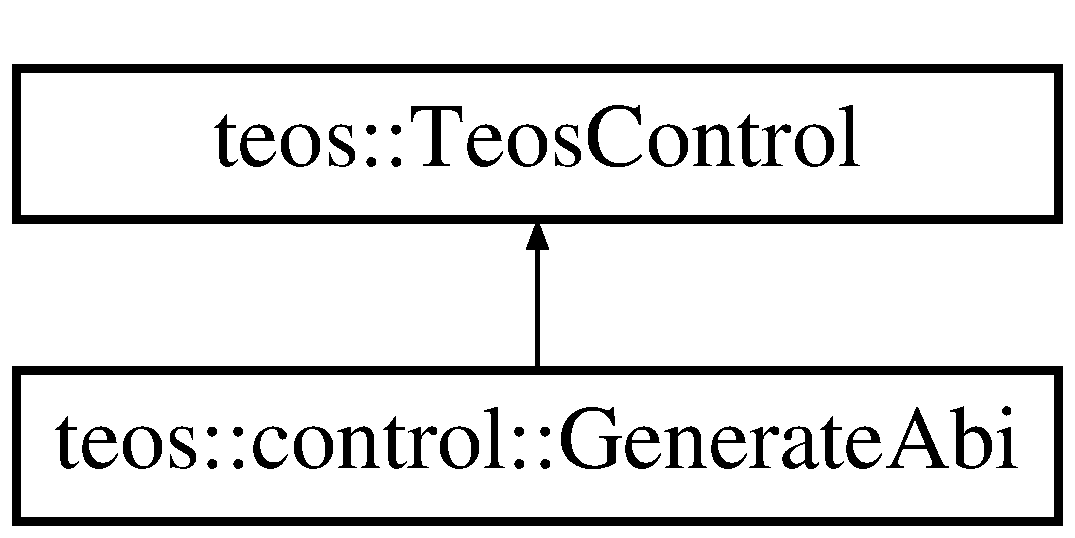
\includegraphics[height=2.000000cm]{classteos_1_1control_1_1_generate_abi}
\end{center}
\end{figure}
\subsection*{Public Member Functions}
\begin{DoxyCompactItemize}
\item 
\mbox{\Hypertarget{classteos_1_1control_1_1_generate_abi_a3306abc2a6f87517aad41efd9ea4ca7e}\label{classteos_1_1control_1_1_generate_abi_a3306abc2a6f87517aad41efd9ea4ca7e}} 
{\bfseries Generate\+Abi} (string types\+\_\+hpp, string abi\+\_\+file=\char`\"{}\char`\"{}, string include\+\_\+dir=\char`\"{}\char`\"{})
\item 
\mbox{\Hypertarget{classteos_1_1control_1_1_generate_abi_ace9ac4a1154f562eb3bb00ff0bc92476}\label{classteos_1_1control_1_1_generate_abi_ace9ac4a1154f562eb3bb00ff0bc92476}} 
{\bfseries Generate\+Abi} (ptree req\+Json)
\end{DoxyCompactItemize}
\subsection*{Additional Inherited Members}


\subsection{Detailed Description}
Generates abi\+: produces the A\+BI file. 

The documentation for this class was generated from the following files\+:\begin{DoxyCompactItemize}
\item 
teos\+\_\+lib/include/teoslib/control/build\+\_\+contract.\+hpp\item 
teos\+\_\+lib/control/build\+\_\+contract.\+cpp\end{DoxyCompactItemize}

\hypertarget{classteos_1_1control_1_1_generate_abi_options}{}\section{teos\+:\+:control\+:\+:Generate\+Abi\+Options Class Reference}
\label{classteos_1_1control_1_1_generate_abi_options}\index{teos\+::control\+::\+Generate\+Abi\+Options@{teos\+::control\+::\+Generate\+Abi\+Options}}


{\ttfamily \#include $<$build\+\_\+contract.\+hpp$>$}

Inheritance diagram for teos\+:\+:control\+:\+:Generate\+Abi\+Options\+:\begin{figure}[H]
\begin{center}
\leavevmode
\includegraphics[height=2.000000cm]{classteos_1_1control_1_1_generate_abi_options}
\end{center}
\end{figure}
\subsection*{Public Member Functions}
\begin{DoxyCompactItemize}
\item 
\mbox{\Hypertarget{classteos_1_1control_1_1_generate_abi_options_addfa748467e9f424013802106132924a}\label{classteos_1_1control_1_1_generate_abi_options_addfa748467e9f424013802106132924a}} 
{\bfseries Generate\+Abi\+Options} (int argc, const char $\ast$$\ast$argv)
\end{DoxyCompactItemize}
\subsection*{Protected Member Functions}
\begin{DoxyCompactItemize}
\item 
const char $\ast$ \mbox{\hyperlink{classteos_1_1control_1_1_generate_abi_options_a7d2ce1ad86518ee06e0bc5ffbe104b39}{get\+Usage}} ()
\begin{DoxyCompactList}\small\item\em Command \textquotesingle{}usage\textquotesingle{} instruction. \end{DoxyCompactList}\item 
\mbox{\Hypertarget{classteos_1_1control_1_1_generate_abi_options_a86ec12899f14876d6d565b4348fc24bb}\label{classteos_1_1control_1_1_generate_abi_options_a86ec12899f14876d6d565b4348fc24bb}} 
options\+\_\+description {\bfseries argument\+Description} ()
\item 
\mbox{\Hypertarget{classteos_1_1control_1_1_generate_abi_options_a8597accc230c49304e2a361484d846f5}\label{classteos_1_1control_1_1_generate_abi_options_a8597accc230c49304e2a361484d846f5}} 
void {\bfseries set\+Pos\+Desc} (positional\+\_\+options\+\_\+description \&pos\+\_\+desc)
\item 
\mbox{\Hypertarget{classteos_1_1control_1_1_generate_abi_options_a1076eeeb66914d7e9580fff26057729b}\label{classteos_1_1control_1_1_generate_abi_options_a1076eeeb66914d7e9580fff26057729b}} 
bool {\bfseries check\+Arguments} (variables\+\_\+map \&vm)
\item 
\mbox{\Hypertarget{classteos_1_1control_1_1_generate_abi_options_a4c059549817da0d83c0ef57f7c98bff9}\label{classteos_1_1control_1_1_generate_abi_options_a4c059549817da0d83c0ef57f7c98bff9}} 
\mbox{\hyperlink{classteos_1_1_teos_control}{Teos\+Control}} {\bfseries execute\+Command} ()
\item 
\mbox{\Hypertarget{classteos_1_1control_1_1_generate_abi_options_a035931ecc56a06cd443ad050ff8bcc8b}\label{classteos_1_1control_1_1_generate_abi_options_a035931ecc56a06cd443ad050ff8bcc8b}} 
void {\bfseries printout} (\mbox{\hyperlink{classteos_1_1_teos_control}{Teos\+Control}} command, variables\+\_\+map \&vm)
\end{DoxyCompactItemize}
\subsection*{Protected Attributes}
\begin{DoxyCompactItemize}
\item 
\mbox{\Hypertarget{classteos_1_1control_1_1_generate_abi_options_a661e9e486d3bc90fd0bff3cffdf125e5}\label{classteos_1_1control_1_1_generate_abi_options_a661e9e486d3bc90fd0bff3cffdf125e5}} 
string {\bfseries types\+\_\+hpp}
\item 
\mbox{\Hypertarget{classteos_1_1control_1_1_generate_abi_options_a038e318e87dd16fbbdf30ec4611d7622}\label{classteos_1_1control_1_1_generate_abi_options_a038e318e87dd16fbbdf30ec4611d7622}} 
string {\bfseries abi\+\_\+file}
\item 
\mbox{\Hypertarget{classteos_1_1control_1_1_generate_abi_options_ac5c99cb639c2ef403673bf8e02c11baf}\label{classteos_1_1control_1_1_generate_abi_options_ac5c99cb639c2ef403673bf8e02c11baf}} 
string {\bfseries include\+\_\+dir}
\end{DoxyCompactItemize}


\subsection{Detailed Description}
Command-\/line driver for the \mbox{\hyperlink{classteos_1_1control_1_1_generate_abi}{Generate\+Abi}} class. 

\subsection{Member Function Documentation}
\mbox{\Hypertarget{classteos_1_1control_1_1_generate_abi_options_a7d2ce1ad86518ee06e0bc5ffbe104b39}\label{classteos_1_1control_1_1_generate_abi_options_a7d2ce1ad86518ee06e0bc5ffbe104b39}} 
\index{teos\+::control\+::\+Generate\+Abi\+Options@{teos\+::control\+::\+Generate\+Abi\+Options}!get\+Usage@{get\+Usage}}
\index{get\+Usage@{get\+Usage}!teos\+::control\+::\+Generate\+Abi\+Options@{teos\+::control\+::\+Generate\+Abi\+Options}}
\subsubsection{\texorpdfstring{get\+Usage()}{getUsage()}}
{\footnotesize\ttfamily const char$\ast$ teos\+::control\+::\+Generate\+Abi\+Options\+::get\+Usage (\begin{DoxyParamCaption}{ }\end{DoxyParamCaption})\hspace{0.3cm}{\ttfamily [inline]}, {\ttfamily [protected]}, {\ttfamily [virtual]}}



Command \textquotesingle{}usage\textquotesingle{} instruction. 

\begin{DoxyReturn}{Returns}
usage text 
\end{DoxyReturn}


Reimplemented from \mbox{\hyperlink{classteos_1_1_control_options_a0aa5671f9bc750ed5280c26c543874f3}{teos\+::\+Control\+Options}}.



The documentation for this class was generated from the following file\+:\begin{DoxyCompactItemize}
\item 
teos\+\_\+lib/include/teoslib/control/build\+\_\+contract.\+hpp\end{DoxyCompactItemize}

\hypertarget{classteos_1_1command_1_1_get_account}{}\section{teos\+:\+:command\+:\+:Get\+Account Class Reference}
\label{classteos_1_1command_1_1_get_account}\index{teos\+::command\+::\+Get\+Account@{teos\+::command\+::\+Get\+Account}}


Fetch a blockchain account.  




{\ttfamily \#include $<$get\+\_\+commands.\+hpp$>$}

Inheritance diagram for teos\+:\+:command\+:\+:Get\+Account\+:\begin{figure}[H]
\begin{center}
\leavevmode
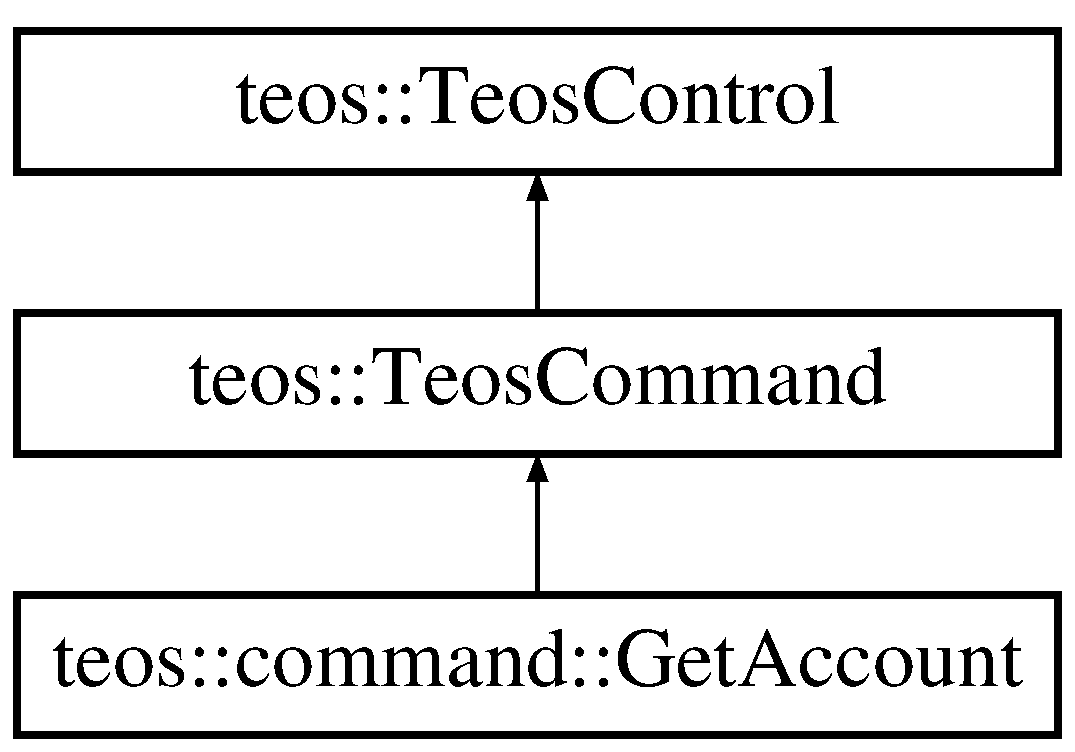
\includegraphics[height=3.000000cm]{classteos_1_1command_1_1_get_account}
\end{center}
\end{figure}
\subsection*{Public Member Functions}
\begin{DoxyCompactItemize}
\item 
\mbox{\Hypertarget{classteos_1_1command_1_1_get_account_a0e9c495d0f86bda5a8c873a57ce12102}\label{classteos_1_1command_1_1_get_account_a0e9c495d0f86bda5a8c873a57ce12102}} 
{\bfseries Get\+Account} (string account\+Name, bool raw=false)
\item 
\mbox{\Hypertarget{classteos_1_1command_1_1_get_account_a57e08f7a17e9d02a886cea53bcce0ce7}\label{classteos_1_1command_1_1_get_account_a57e08f7a17e9d02a886cea53bcce0ce7}} 
{\bfseries Get\+Account} (ptree req\+Json, bool raw=false)
\end{DoxyCompactItemize}
\subsection*{Additional Inherited Members}


\subsection{Detailed Description}
Fetch a blockchain account. 

The documentation for this class was generated from the following file\+:\begin{DoxyCompactItemize}
\item 
teos\+\_\+lib/include/teoslib/command/\mbox{\hyperlink{get__commands_8hpp}{get\+\_\+commands.\+hpp}}\end{DoxyCompactItemize}

\hypertarget{classteos_1_1command_1_1_get_account_options}{}\section{teos\+:\+:command\+:\+:Get\+Account\+Options Class Reference}
\label{classteos_1_1command_1_1_get_account_options}\index{teos\+::command\+::\+Get\+Account\+Options@{teos\+::command\+::\+Get\+Account\+Options}}


Command-\/line driver for the \mbox{\hyperlink{classteos_1_1command_1_1_get_account}{Get\+Account}} class.  




{\ttfamily \#include $<$get\+\_\+commands.\+hpp$>$}

Inheritance diagram for teos\+:\+:command\+:\+:Get\+Account\+Options\+:\begin{figure}[H]
\begin{center}
\leavevmode
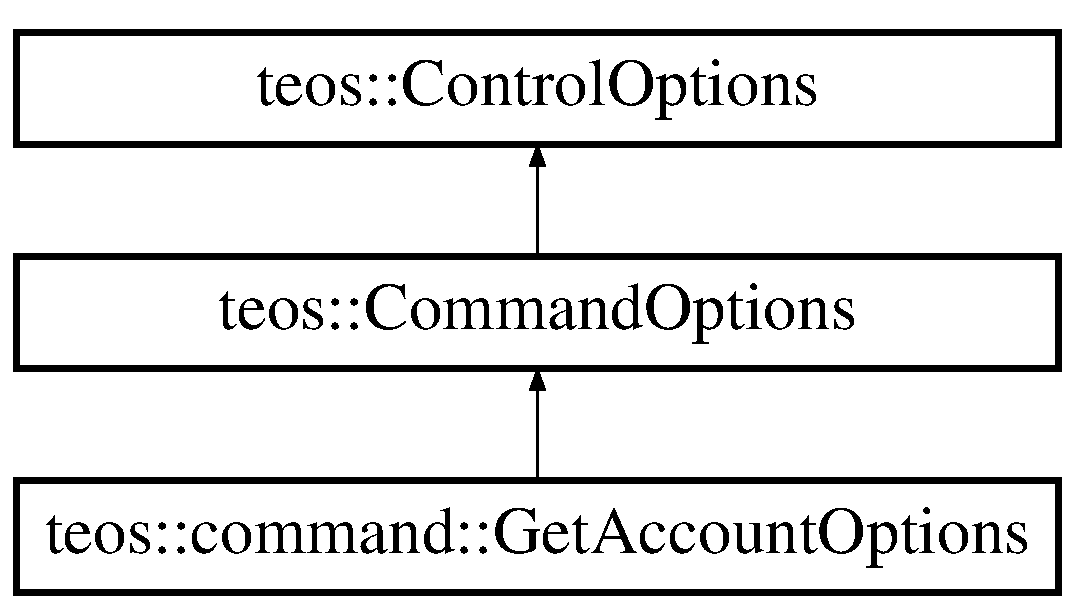
\includegraphics[height=3.000000cm]{classteos_1_1command_1_1_get_account_options}
\end{center}
\end{figure}
\subsection*{Public Member Functions}
\begin{DoxyCompactItemize}
\item 
\mbox{\Hypertarget{classteos_1_1command_1_1_get_account_options_a8a932086b050c3446bd371293b7ea534}\label{classteos_1_1command_1_1_get_account_options_a8a932086b050c3446bd371293b7ea534}} 
{\bfseries Get\+Account\+Options} (int argc, const char $\ast$$\ast$argv)
\end{DoxyCompactItemize}
\subsection*{Protected Member Functions}
\begin{DoxyCompactItemize}
\item 
const char $\ast$ \mbox{\hyperlink{classteos_1_1command_1_1_get_account_options_a987381bcf3f687b7babfe197edf0dc26}{get\+Usage}} ()
\begin{DoxyCompactList}\small\item\em Command \textquotesingle{}usage\textquotesingle{} instruction. \end{DoxyCompactList}\item 
\mbox{\Hypertarget{classteos_1_1command_1_1_get_account_options_a91575b9022b083326ed27cce53838f19}\label{classteos_1_1command_1_1_get_account_options_a91575b9022b083326ed27cce53838f19}} 
options\+\_\+description {\bfseries argument\+Description} ()
\item 
\mbox{\Hypertarget{classteos_1_1command_1_1_get_account_options_a58476192130fc6ec9e08ef9aabbc6940}\label{classteos_1_1command_1_1_get_account_options_a58476192130fc6ec9e08ef9aabbc6940}} 
void {\bfseries set\+Pos\+Desc} (positional\+\_\+options\+\_\+description \&pos\+\_\+desc)
\item 
\mbox{\Hypertarget{classteos_1_1command_1_1_get_account_options_a6ffd8f40413adfcb07e8b4fecffe5bc2}\label{classteos_1_1command_1_1_get_account_options_a6ffd8f40413adfcb07e8b4fecffe5bc2}} 
bool {\bfseries check\+Arguments} (variables\+\_\+map \&vm)
\item 
\mbox{\Hypertarget{classteos_1_1command_1_1_get_account_options_a03ae1a974c59a3942d965ddf9fb56ae3}\label{classteos_1_1command_1_1_get_account_options_a03ae1a974c59a3942d965ddf9fb56ae3}} 
\mbox{\hyperlink{classteos_1_1_teos_control}{Teos\+Control}} {\bfseries execute\+Command} ()
\item 
\mbox{\Hypertarget{classteos_1_1command_1_1_get_account_options_afafce99b027588616f736949ae051272}\label{classteos_1_1command_1_1_get_account_options_afafce99b027588616f736949ae051272}} 
void {\bfseries printout} (\mbox{\hyperlink{classteos_1_1_teos_control}{Teos\+Control}} command, variables\+\_\+map \&vm)
\end{DoxyCompactItemize}
\subsection*{Protected Attributes}
\begin{DoxyCompactItemize}
\item 
\mbox{\Hypertarget{classteos_1_1command_1_1_get_account_options_a6ac4d44162e66da311de6a9055b8975c}\label{classteos_1_1command_1_1_get_account_options_a6ac4d44162e66da311de6a9055b8975c}} 
string {\bfseries name}
\end{DoxyCompactItemize}
\subsection*{Additional Inherited Members}


\subsection{Detailed Description}
Command-\/line driver for the \mbox{\hyperlink{classteos_1_1command_1_1_get_account}{Get\+Account}} class. 

\subsection{Member Function Documentation}
\mbox{\Hypertarget{classteos_1_1command_1_1_get_account_options_a987381bcf3f687b7babfe197edf0dc26}\label{classteos_1_1command_1_1_get_account_options_a987381bcf3f687b7babfe197edf0dc26}} 
\index{teos\+::command\+::\+Get\+Account\+Options@{teos\+::command\+::\+Get\+Account\+Options}!get\+Usage@{get\+Usage}}
\index{get\+Usage@{get\+Usage}!teos\+::command\+::\+Get\+Account\+Options@{teos\+::command\+::\+Get\+Account\+Options}}
\subsubsection{\texorpdfstring{get\+Usage()}{getUsage()}}
{\footnotesize\ttfamily const char$\ast$ teos\+::command\+::\+Get\+Account\+Options\+::get\+Usage (\begin{DoxyParamCaption}{ }\end{DoxyParamCaption})\hspace{0.3cm}{\ttfamily [inline]}, {\ttfamily [protected]}, {\ttfamily [virtual]}}



Command \textquotesingle{}usage\textquotesingle{} instruction. 

\begin{DoxyReturn}{Returns}
usage text 
\end{DoxyReturn}


Reimplemented from \mbox{\hyperlink{classteos_1_1_control_options_a0aa5671f9bc750ed5280c26c543874f3}{teos\+::\+Control\+Options}}.



The documentation for this class was generated from the following file\+:\begin{DoxyCompactItemize}
\item 
teos\+\_\+lib/include/teoslib/command/\mbox{\hyperlink{get__commands_8hpp}{get\+\_\+commands.\+hpp}}\end{DoxyCompactItemize}

\hypertarget{classteos_1_1command_1_1_get_accounts}{}\section{teos\+:\+:command\+:\+:Get\+Accounts Class Reference}
\label{classteos_1_1command_1_1_get_accounts}\index{teos\+::command\+::\+Get\+Accounts@{teos\+::command\+::\+Get\+Accounts}}


Retrieve accounts associated with a public key.  




{\ttfamily \#include $<$get\+\_\+commands.\+hpp$>$}

Inheritance diagram for teos\+:\+:command\+:\+:Get\+Accounts\+:\begin{figure}[H]
\begin{center}
\leavevmode
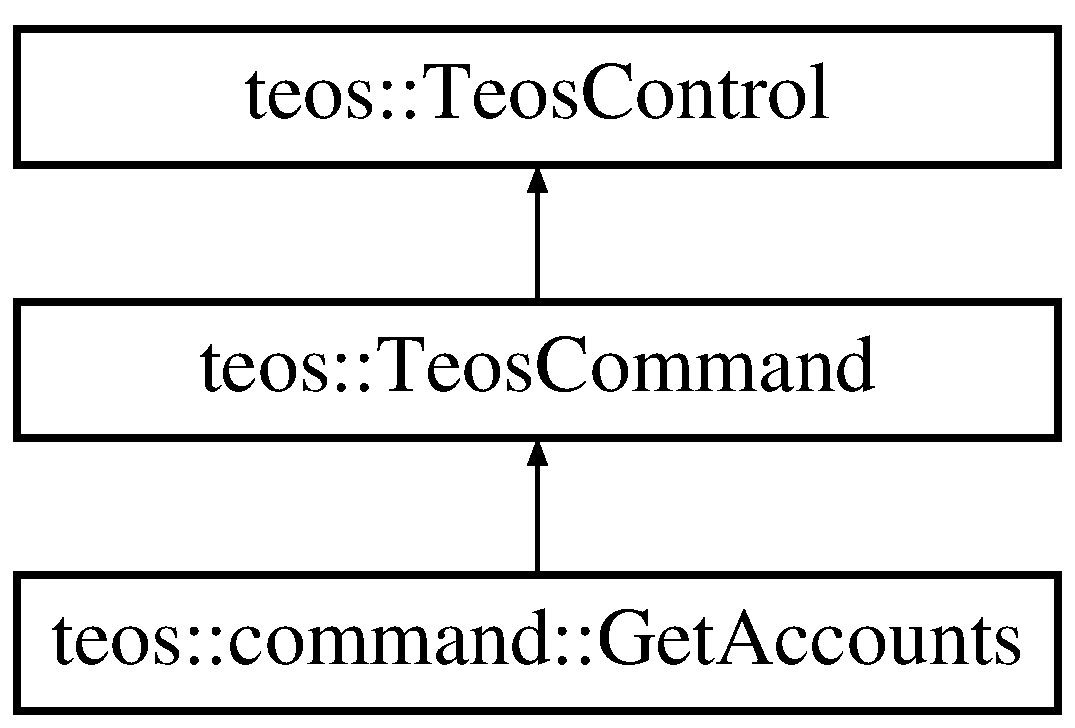
\includegraphics[height=3.000000cm]{classteos_1_1command_1_1_get_accounts}
\end{center}
\end{figure}
\subsection*{Public Member Functions}
\begin{DoxyCompactItemize}
\item 
\mbox{\Hypertarget{classteos_1_1command_1_1_get_accounts_a603eb927fd9617cb566e20a550a399ee}\label{classteos_1_1command_1_1_get_accounts_a603eb927fd9617cb566e20a550a399ee}} 
{\bfseries Get\+Accounts} (string public\+Key)
\item 
\mbox{\Hypertarget{classteos_1_1command_1_1_get_accounts_aafacb3452faaab3051b2b2876461c01d}\label{classteos_1_1command_1_1_get_accounts_aafacb3452faaab3051b2b2876461c01d}} 
{\bfseries Get\+Accounts} (ptree req\+Json)
\end{DoxyCompactItemize}
\subsection*{Additional Inherited Members}


\subsection{Detailed Description}
Retrieve accounts associated with a public key. 

The documentation for this class was generated from the following file\+:\begin{DoxyCompactItemize}
\item 
include/teoslib/command/\mbox{\hyperlink{get__commands_8hpp}{get\+\_\+commands.\+hpp}}\end{DoxyCompactItemize}

\hypertarget{classteos_1_1command_1_1_get_accounts_options}{}\section{teos\+:\+:command\+:\+:Get\+Accounts\+Options Class Reference}
\label{classteos_1_1command_1_1_get_accounts_options}\index{teos\+::command\+::\+Get\+Accounts\+Options@{teos\+::command\+::\+Get\+Accounts\+Options}}


Command-\/line driver for the \mbox{\hyperlink{classteos_1_1command_1_1_get_accounts}{Get\+Accounts}} class.  




{\ttfamily \#include $<$get\+\_\+commands.\+hpp$>$}

Inheritance diagram for teos\+:\+:command\+:\+:Get\+Accounts\+Options\+:\begin{figure}[H]
\begin{center}
\leavevmode
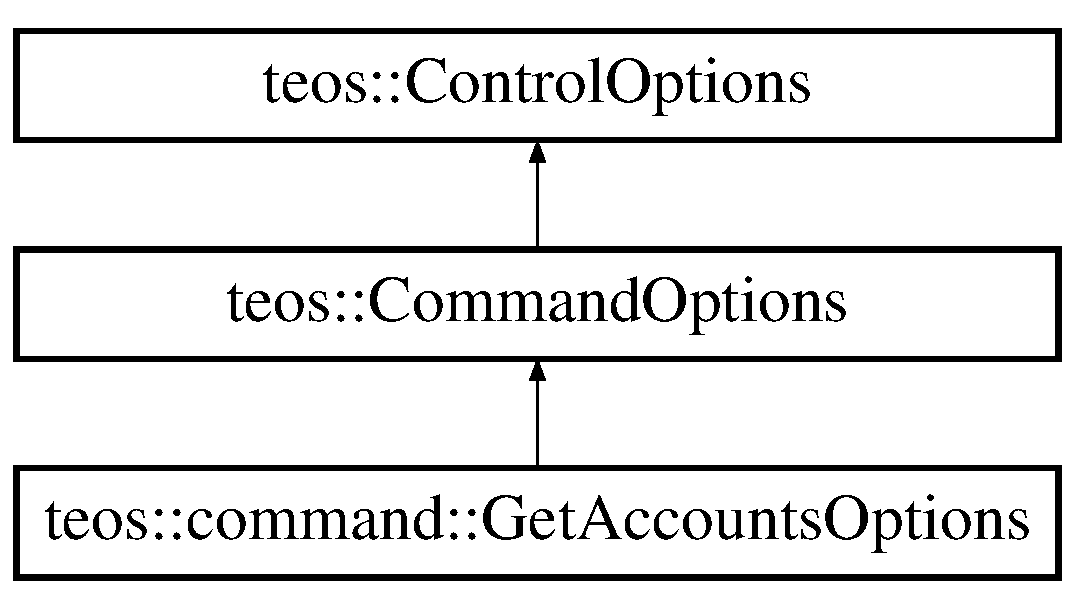
\includegraphics[height=3.000000cm]{classteos_1_1command_1_1_get_accounts_options}
\end{center}
\end{figure}
\subsection*{Public Member Functions}
\begin{DoxyCompactItemize}
\item 
\mbox{\Hypertarget{classteos_1_1command_1_1_get_accounts_options_a2323a4efff47895e79f63f191a3c42d1}\label{classteos_1_1command_1_1_get_accounts_options_a2323a4efff47895e79f63f191a3c42d1}} 
{\bfseries Get\+Accounts\+Options} (int argc, const char $\ast$$\ast$argv)
\end{DoxyCompactItemize}
\subsection*{Protected Member Functions}
\begin{DoxyCompactItemize}
\item 
const char $\ast$ \mbox{\hyperlink{classteos_1_1command_1_1_get_accounts_options_ac93b806fa601124aa899474da62d1288}{get\+Usage}} ()
\begin{DoxyCompactList}\small\item\em Command \textquotesingle{}usage\textquotesingle{} instruction. \end{DoxyCompactList}\item 
\mbox{\Hypertarget{classteos_1_1command_1_1_get_accounts_options_a895c2708a09db687d738aa215fcb2ce9}\label{classteos_1_1command_1_1_get_accounts_options_a895c2708a09db687d738aa215fcb2ce9}} 
options\+\_\+description {\bfseries argument\+Description} ()
\item 
\mbox{\Hypertarget{classteos_1_1command_1_1_get_accounts_options_af8bd3d166447f342a64f676a9d2437da}\label{classteos_1_1command_1_1_get_accounts_options_af8bd3d166447f342a64f676a9d2437da}} 
void {\bfseries set\+Pos\+Desc} (positional\+\_\+options\+\_\+description \&pos\+\_\+desc)
\item 
\mbox{\Hypertarget{classteos_1_1command_1_1_get_accounts_options_a3c31f6264e33997c8f17475755d69861}\label{classteos_1_1command_1_1_get_accounts_options_a3c31f6264e33997c8f17475755d69861}} 
bool {\bfseries check\+Arguments} (variables\+\_\+map \&vm)
\item 
\mbox{\Hypertarget{classteos_1_1command_1_1_get_accounts_options_ad6e48fb73341c5469ce56558da5adc87}\label{classteos_1_1command_1_1_get_accounts_options_ad6e48fb73341c5469ce56558da5adc87}} 
\mbox{\hyperlink{classteos_1_1_teos_control}{Teos\+Control}} {\bfseries execute\+Command} ()
\end{DoxyCompactItemize}
\subsection*{Protected Attributes}
\begin{DoxyCompactItemize}
\item 
\mbox{\Hypertarget{classteos_1_1command_1_1_get_accounts_options_ac25b9f603525d685116441334d61a973}\label{classteos_1_1command_1_1_get_accounts_options_ac25b9f603525d685116441334d61a973}} 
string {\bfseries public\+\_\+key}
\end{DoxyCompactItemize}
\subsection*{Additional Inherited Members}


\subsection{Detailed Description}
Command-\/line driver for the \mbox{\hyperlink{classteos_1_1command_1_1_get_accounts}{Get\+Accounts}} class. 

\subsection{Member Function Documentation}
\mbox{\Hypertarget{classteos_1_1command_1_1_get_accounts_options_ac93b806fa601124aa899474da62d1288}\label{classteos_1_1command_1_1_get_accounts_options_ac93b806fa601124aa899474da62d1288}} 
\index{teos\+::command\+::\+Get\+Accounts\+Options@{teos\+::command\+::\+Get\+Accounts\+Options}!get\+Usage@{get\+Usage}}
\index{get\+Usage@{get\+Usage}!teos\+::command\+::\+Get\+Accounts\+Options@{teos\+::command\+::\+Get\+Accounts\+Options}}
\subsubsection{\texorpdfstring{get\+Usage()}{getUsage()}}
{\footnotesize\ttfamily const char$\ast$ teos\+::command\+::\+Get\+Accounts\+Options\+::get\+Usage (\begin{DoxyParamCaption}{ }\end{DoxyParamCaption})\hspace{0.3cm}{\ttfamily [inline]}, {\ttfamily [protected]}, {\ttfamily [virtual]}}



Command \textquotesingle{}usage\textquotesingle{} instruction. 

\begin{DoxyReturn}{Returns}
usage text 
\end{DoxyReturn}


Reimplemented from \mbox{\hyperlink{classteos_1_1_control_options_a0aa5671f9bc750ed5280c26c543874f3}{teos\+::\+Control\+Options}}.



The documentation for this class was generated from the following file\+:\begin{DoxyCompactItemize}
\item 
include/teoslib/command/\mbox{\hyperlink{get__commands_8hpp}{get\+\_\+commands.\+hpp}}\end{DoxyCompactItemize}

\hypertarget{classteos_1_1command_1_1_get_block}{}\section{teos\+:\+:command\+:\+:Get\+Block Class Reference}
\label{classteos_1_1command_1_1_get_block}\index{teos\+::command\+::\+Get\+Block@{teos\+::command\+::\+Get\+Block}}


Retrieve a full block from a blockchain.  




{\ttfamily \#include $<$get\+\_\+commands.\+hpp$>$}

Inheritance diagram for teos\+:\+:command\+:\+:Get\+Block\+:\begin{figure}[H]
\begin{center}
\leavevmode
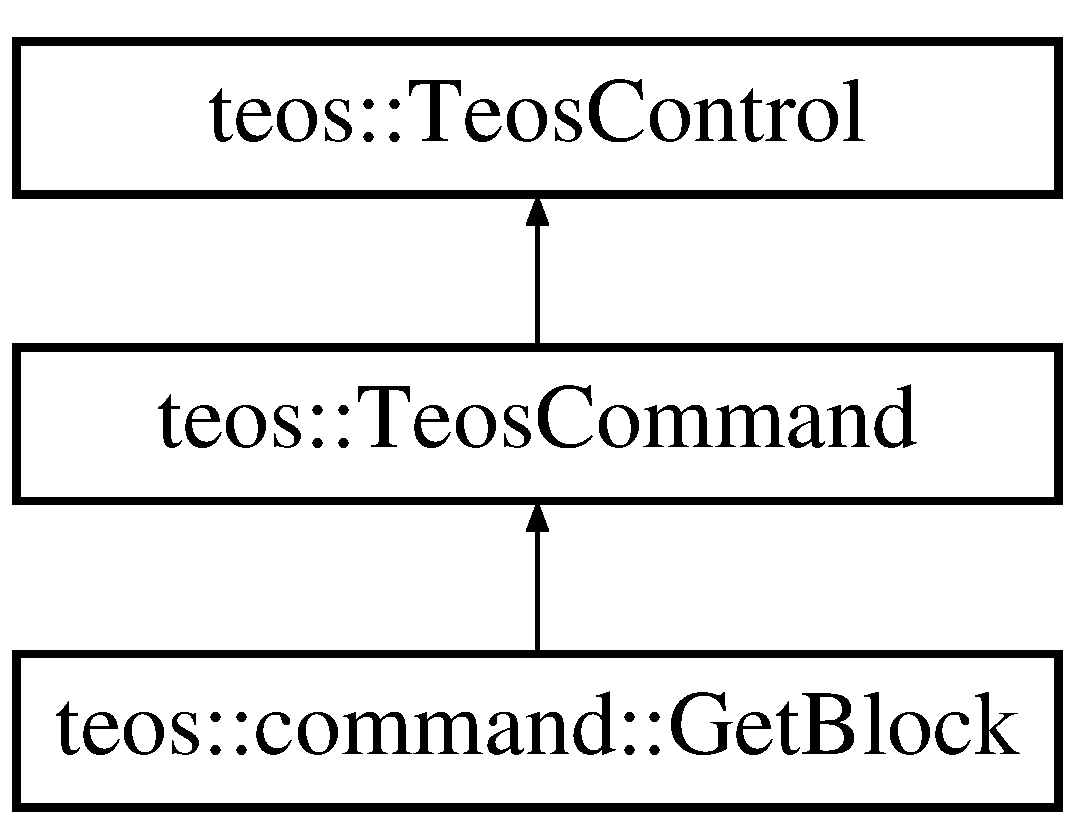
\includegraphics[height=3.000000cm]{classteos_1_1command_1_1_get_block}
\end{center}
\end{figure}
\subsection*{Public Member Functions}
\begin{DoxyCompactItemize}
\item 
\mbox{\Hypertarget{classteos_1_1command_1_1_get_block_a2e422461f3a01ea1f1514f69b3a55fec}\label{classteos_1_1command_1_1_get_block_a2e422461f3a01ea1f1514f69b3a55fec}} 
{\bfseries Get\+Block} (ptree req\+Json, bool raw=false)
\end{DoxyCompactItemize}
\subsection*{Additional Inherited Members}


\subsection{Detailed Description}
Retrieve a full block from a blockchain. 

The documentation for this class was generated from the following file\+:\begin{DoxyCompactItemize}
\item 
teos\+\_\+lib/include/teoslib/command/\mbox{\hyperlink{get__commands_8hpp}{get\+\_\+commands.\+hpp}}\end{DoxyCompactItemize}

\hypertarget{classteos_1_1command_1_1_get_block_options}{}\section{teos\+:\+:command\+:\+:Get\+Block\+Options Class Reference}
\label{classteos_1_1command_1_1_get_block_options}\index{teos\+::command\+::\+Get\+Block\+Options@{teos\+::command\+::\+Get\+Block\+Options}}


Command-\/line driver for the \mbox{\hyperlink{classteos_1_1command_1_1_get_block}{Get\+Block}} class.  




{\ttfamily \#include $<$get\+\_\+commands.\+hpp$>$}

Inheritance diagram for teos\+:\+:command\+:\+:Get\+Block\+Options\+:\begin{figure}[H]
\begin{center}
\leavevmode
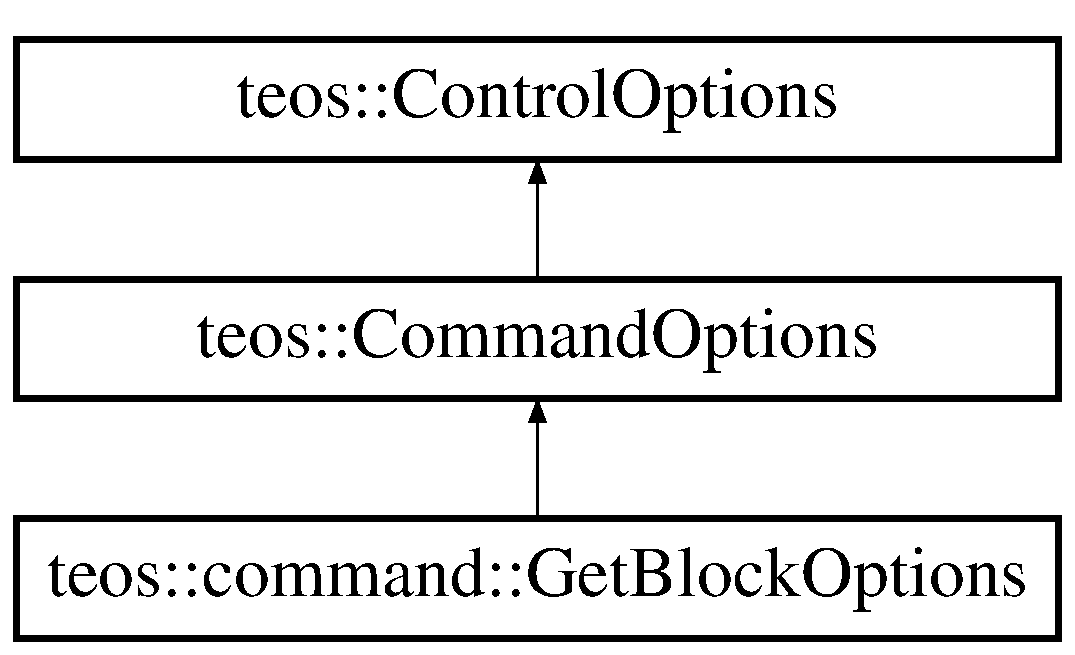
\includegraphics[height=3.000000cm]{classteos_1_1command_1_1_get_block_options}
\end{center}
\end{figure}
\subsection*{Public Member Functions}
\begin{DoxyCompactItemize}
\item 
\mbox{\Hypertarget{classteos_1_1command_1_1_get_block_options_ad9e83d4b0beddabb25ee7089ae8ef55a}\label{classteos_1_1command_1_1_get_block_options_ad9e83d4b0beddabb25ee7089ae8ef55a}} 
{\bfseries Get\+Block\+Options} (int argc, const char $\ast$$\ast$argv)
\end{DoxyCompactItemize}
\subsection*{Protected Member Functions}
\begin{DoxyCompactItemize}
\item 
const char $\ast$ \mbox{\hyperlink{classteos_1_1command_1_1_get_block_options_a85970d4f6337e594d2ac0756f67c50f7}{get\+Usage}} ()
\begin{DoxyCompactList}\small\item\em Command \textquotesingle{}usage\textquotesingle{} instruction. \end{DoxyCompactList}\item 
\mbox{\Hypertarget{classteos_1_1command_1_1_get_block_options_a5a68a8f531b223e6a9d3ee72333310c8}\label{classteos_1_1command_1_1_get_block_options_a5a68a8f531b223e6a9d3ee72333310c8}} 
options\+\_\+description {\bfseries argument\+Description} ()
\item 
\mbox{\Hypertarget{classteos_1_1command_1_1_get_block_options_abce9cbc2c1454d56975ad12be740bd8f}\label{classteos_1_1command_1_1_get_block_options_abce9cbc2c1454d56975ad12be740bd8f}} 
void {\bfseries set\+Pos\+Desc} (positional\+\_\+options\+\_\+description \&pos\+\_\+desc)
\item 
\mbox{\Hypertarget{classteos_1_1command_1_1_get_block_options_a081cfcc951b0f47a30dea915c9daea5e}\label{classteos_1_1command_1_1_get_block_options_a081cfcc951b0f47a30dea915c9daea5e}} 
bool {\bfseries check\+Arguments} (variables\+\_\+map \&vm)
\item 
\mbox{\Hypertarget{classteos_1_1command_1_1_get_block_options_a58079b3a605d0873679df019e882ead3}\label{classteos_1_1command_1_1_get_block_options_a58079b3a605d0873679df019e882ead3}} 
\mbox{\hyperlink{classteos_1_1_teos_control}{Teos\+Control}} {\bfseries execute\+Command} ()
\item 
\mbox{\Hypertarget{classteos_1_1command_1_1_get_block_options_a5e74ced61b77ec00dc565baa269dee02}\label{classteos_1_1command_1_1_get_block_options_a5e74ced61b77ec00dc565baa269dee02}} 
void {\bfseries printout} (\mbox{\hyperlink{classteos_1_1_teos_control}{Teos\+Control}} command, variables\+\_\+map \&vm)
\end{DoxyCompactItemize}
\subsection*{Protected Attributes}
\begin{DoxyCompactItemize}
\item 
\mbox{\Hypertarget{classteos_1_1command_1_1_get_block_options_ad39586d70ad06d302556ccbc65a32171}\label{classteos_1_1command_1_1_get_block_options_ad39586d70ad06d302556ccbc65a32171}} 
int {\bfseries n}
\item 
\mbox{\Hypertarget{classteos_1_1command_1_1_get_block_options_aca9d966ac2b724944a3e664689e68995}\label{classteos_1_1command_1_1_get_block_options_aca9d966ac2b724944a3e664689e68995}} 
string {\bfseries id}
\end{DoxyCompactItemize}
\subsection*{Additional Inherited Members}


\subsection{Detailed Description}
Command-\/line driver for the \mbox{\hyperlink{classteos_1_1command_1_1_get_block}{Get\+Block}} class. 

\subsection{Member Function Documentation}
\mbox{\Hypertarget{classteos_1_1command_1_1_get_block_options_a85970d4f6337e594d2ac0756f67c50f7}\label{classteos_1_1command_1_1_get_block_options_a85970d4f6337e594d2ac0756f67c50f7}} 
\index{teos\+::command\+::\+Get\+Block\+Options@{teos\+::command\+::\+Get\+Block\+Options}!get\+Usage@{get\+Usage}}
\index{get\+Usage@{get\+Usage}!teos\+::command\+::\+Get\+Block\+Options@{teos\+::command\+::\+Get\+Block\+Options}}
\subsubsection{\texorpdfstring{get\+Usage()}{getUsage()}}
{\footnotesize\ttfamily const char$\ast$ teos\+::command\+::\+Get\+Block\+Options\+::get\+Usage (\begin{DoxyParamCaption}{ }\end{DoxyParamCaption})\hspace{0.3cm}{\ttfamily [inline]}, {\ttfamily [protected]}, {\ttfamily [virtual]}}



Command \textquotesingle{}usage\textquotesingle{} instruction. 

\begin{DoxyReturn}{Returns}
usage text 
\end{DoxyReturn}


Reimplemented from \mbox{\hyperlink{classteos_1_1_control_options_a0aa5671f9bc750ed5280c26c543874f3}{teos\+::\+Control\+Options}}.



The documentation for this class was generated from the following file\+:\begin{DoxyCompactItemize}
\item 
include/teoslib/command/\mbox{\hyperlink{get__commands_8hpp}{get\+\_\+commands.\+hpp}}\end{DoxyCompactItemize}

\hypertarget{classteos_1_1command_1_1_get_code}{}\section{teos\+:\+:command\+:\+:Get\+Code Class Reference}
\label{classteos_1_1command_1_1_get_code}\index{teos\+::command\+::\+Get\+Code@{teos\+::command\+::\+Get\+Code}}


Retrieves the code and A\+BI for an account.  




{\ttfamily \#include $<$get\+\_\+commands.\+hpp$>$}

Inheritance diagram for teos\+:\+:command\+:\+:Get\+Code\+:\begin{figure}[H]
\begin{center}
\leavevmode
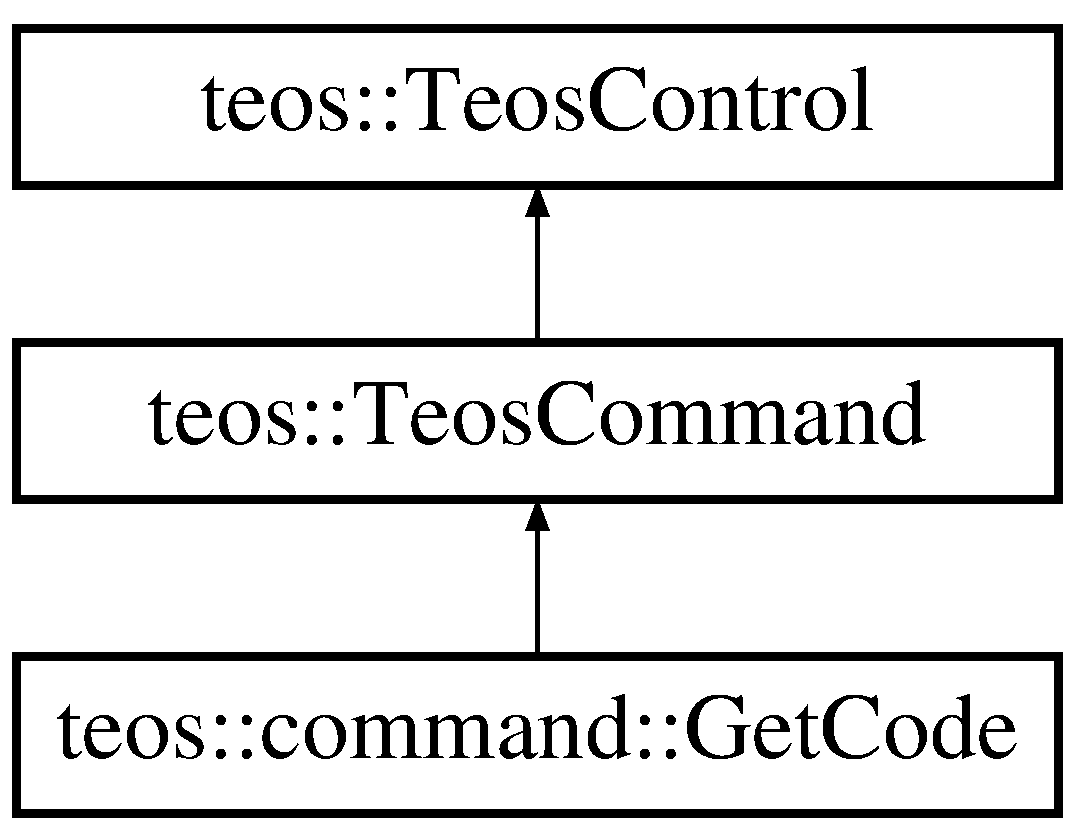
\includegraphics[height=3.000000cm]{classteos_1_1command_1_1_get_code}
\end{center}
\end{figure}
\subsection*{Public Member Functions}
\begin{DoxyCompactItemize}
\item 
\mbox{\hyperlink{classteos_1_1command_1_1_get_code_ac1111aac4926fccc9447c1009aadf299}{Get\+Code}} (string account\+Name, string wast\+File=\char`\"{}\char`\"{}, string abi\+File=\char`\"{}\char`\"{})
\begin{DoxyCompactList}\small\item\em A constructor. \end{DoxyCompactList}\item 
\mbox{\hyperlink{classteos_1_1command_1_1_get_code_aa93979c1ca9b4296ccfc4ea847bd2217}{Get\+Code}} (ptree req\+Json)
\begin{DoxyCompactList}\small\item\em A constructor. \end{DoxyCompactList}\end{DoxyCompactItemize}
\subsection*{Additional Inherited Members}


\subsection{Detailed Description}
Retrieves the code and A\+BI for an account. 

\subsection{Constructor \& Destructor Documentation}
\mbox{\Hypertarget{classteos_1_1command_1_1_get_code_ac1111aac4926fccc9447c1009aadf299}\label{classteos_1_1command_1_1_get_code_ac1111aac4926fccc9447c1009aadf299}} 
\index{teos\+::command\+::\+Get\+Code@{teos\+::command\+::\+Get\+Code}!Get\+Code@{Get\+Code}}
\index{Get\+Code@{Get\+Code}!teos\+::command\+::\+Get\+Code@{teos\+::command\+::\+Get\+Code}}
\subsubsection{\texorpdfstring{Get\+Code()}{GetCode()}\hspace{0.1cm}{\footnotesize\ttfamily [1/2]}}
{\footnotesize\ttfamily teos\+::command\+::\+Get\+Code\+::\+Get\+Code (\begin{DoxyParamCaption}\item[{string}]{account\+Name,  }\item[{string}]{wast\+File = {\ttfamily \char`\"{}\char`\"{}},  }\item[{string}]{abi\+File = {\ttfamily \char`\"{}\char`\"{}} }\end{DoxyParamCaption})\hspace{0.3cm}{\ttfamily [inline]}}



A constructor. 


\begin{DoxyParams}{Parameters}
{\em wast\+File} & where write the wast code to. If \char`\"{}\+\_\+\char`\"{}, print to stdout. \\
\hline
{\em abi\+File} & where write the abi code to. If \char`\"{}\+\_\+\char`\"{}, print to stdout. \char`\"{}wast\char`\"{}\+:\char`\"{}$<$\+W\+A\+S\+T code$>$\char`\"{}, \char`\"{}abi\char`\"{}\+:\char`\"{}$<$abi structure$>$\char`\"{}\}. \\
\hline
\end{DoxyParams}
\mbox{\Hypertarget{classteos_1_1command_1_1_get_code_aa93979c1ca9b4296ccfc4ea847bd2217}\label{classteos_1_1command_1_1_get_code_aa93979c1ca9b4296ccfc4ea847bd2217}} 
\index{teos\+::command\+::\+Get\+Code@{teos\+::command\+::\+Get\+Code}!Get\+Code@{Get\+Code}}
\index{Get\+Code@{Get\+Code}!teos\+::command\+::\+Get\+Code@{teos\+::command\+::\+Get\+Code}}
\subsubsection{\texorpdfstring{Get\+Code()}{GetCode()}\hspace{0.1cm}{\footnotesize\ttfamily [2/2]}}
{\footnotesize\ttfamily teos\+::command\+::\+Get\+Code\+::\+Get\+Code (\begin{DoxyParamCaption}\item[{ptree}]{req\+Json }\end{DoxyParamCaption})\hspace{0.3cm}{\ttfamily [inline]}}



A constructor. 


\begin{DoxyParams}{Parameters}
{\em req\+Json} & json tree argument\+: \{\char`\"{}account\+\_\+name\char`\"{}\+:\char`\"{}$<$account name$>$\char`\"{}, \char`\"{}wast\char`\"{}\+:\char`\"{}$<$wast file$>$\char`\"{}, \char`\"{}abi\char`\"{}\+:\char`\"{}$<$abi file$>$\char`\"{}\} \\
\hline
{\em raw} & if true, resulting json is not formated. \\
\hline
\end{DoxyParams}


The documentation for this class was generated from the following file\+:\begin{DoxyCompactItemize}
\item 
include/teoslib/command/\mbox{\hyperlink{get__commands_8hpp}{get\+\_\+commands.\+hpp}}\end{DoxyCompactItemize}

\hypertarget{classteos_1_1command_1_1_get_code_options}{}\section{teos\+:\+:command\+:\+:Get\+Code\+Options Class Reference}
\label{classteos_1_1command_1_1_get_code_options}\index{teos\+::command\+::\+Get\+Code\+Options@{teos\+::command\+::\+Get\+Code\+Options}}


Command-\/line driver for the \mbox{\hyperlink{classteos_1_1command_1_1_get_code}{Get\+Code}} class.  




{\ttfamily \#include $<$get\+\_\+commands.\+hpp$>$}

Inheritance diagram for teos\+:\+:command\+:\+:Get\+Code\+Options\+:\begin{figure}[H]
\begin{center}
\leavevmode
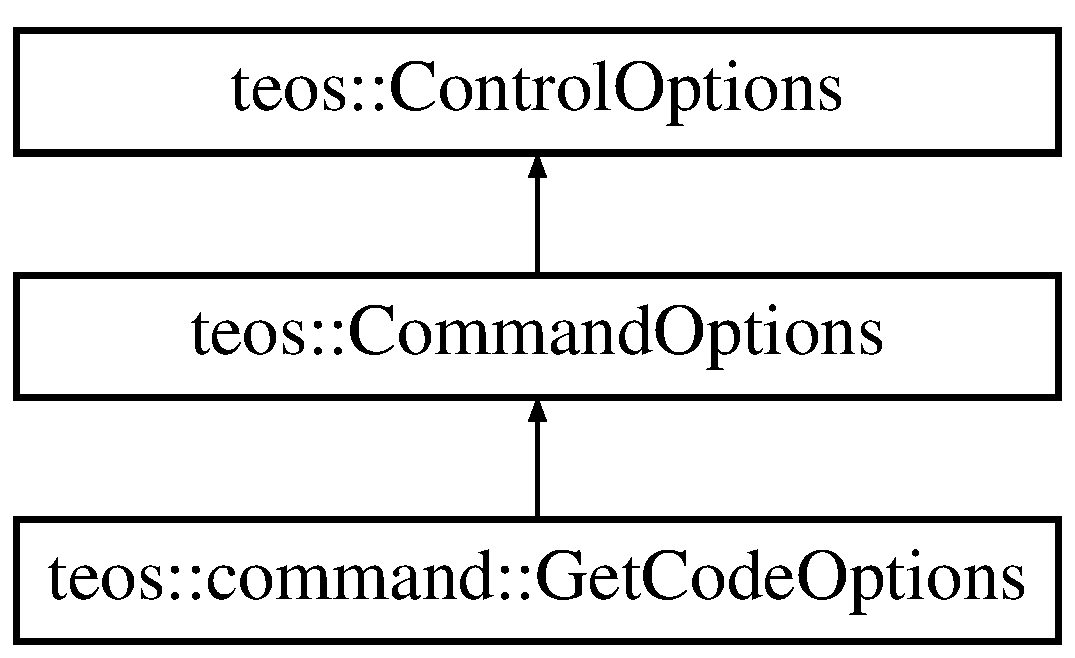
\includegraphics[height=3.000000cm]{classteos_1_1command_1_1_get_code_options}
\end{center}
\end{figure}
\subsection*{Public Member Functions}
\begin{DoxyCompactItemize}
\item 
\mbox{\Hypertarget{classteos_1_1command_1_1_get_code_options_ae378530fd0d71e3317d249166bffb2b9}\label{classteos_1_1command_1_1_get_code_options_ae378530fd0d71e3317d249166bffb2b9}} 
{\bfseries Get\+Code\+Options} (int argc, const char $\ast$$\ast$argv)
\end{DoxyCompactItemize}
\subsection*{Protected Member Functions}
\begin{DoxyCompactItemize}
\item 
const char $\ast$ \mbox{\hyperlink{classteos_1_1command_1_1_get_code_options_a62a3c2c3cc72eb8b9bd5034fb335c7e2}{get\+Usage}} ()
\begin{DoxyCompactList}\small\item\em Command \textquotesingle{}usage\textquotesingle{} instruction. \end{DoxyCompactList}\item 
\mbox{\Hypertarget{classteos_1_1command_1_1_get_code_options_a0cfb2d780f53e27ccc08e8a887d6f053}\label{classteos_1_1command_1_1_get_code_options_a0cfb2d780f53e27ccc08e8a887d6f053}} 
options\+\_\+description {\bfseries argument\+Description} ()
\item 
\mbox{\Hypertarget{classteos_1_1command_1_1_get_code_options_a462d7de6d307c8b87c01a8c458eeb783}\label{classteos_1_1command_1_1_get_code_options_a462d7de6d307c8b87c01a8c458eeb783}} 
void {\bfseries set\+Pos\+Desc} (positional\+\_\+options\+\_\+description \&pos\+\_\+desc)
\item 
\mbox{\Hypertarget{classteos_1_1command_1_1_get_code_options_a1731e3500edcca10b78bfb86f74b5ed9}\label{classteos_1_1command_1_1_get_code_options_a1731e3500edcca10b78bfb86f74b5ed9}} 
bool {\bfseries check\+Arguments} (variables\+\_\+map \&vm)
\item 
\mbox{\Hypertarget{classteos_1_1command_1_1_get_code_options_a53d7ff2b9a882990933bc0a1194f8f28}\label{classteos_1_1command_1_1_get_code_options_a53d7ff2b9a882990933bc0a1194f8f28}} 
\mbox{\hyperlink{classteos_1_1_teos_control}{Teos\+Control}} {\bfseries execute\+Command} ()
\item 
\mbox{\Hypertarget{classteos_1_1command_1_1_get_code_options_ac7390aecf45c00142f7cc008f7b2660f}\label{classteos_1_1command_1_1_get_code_options_ac7390aecf45c00142f7cc008f7b2660f}} 
void {\bfseries printout} (\mbox{\hyperlink{classteos_1_1_teos_control}{Teos\+Control}} command, variables\+\_\+map \&vm)
\end{DoxyCompactItemize}
\subsection*{Protected Attributes}
\begin{DoxyCompactItemize}
\item 
\mbox{\Hypertarget{classteos_1_1command_1_1_get_code_options_a2ccae73659e64448134d2eecddeb21ff}\label{classteos_1_1command_1_1_get_code_options_a2ccae73659e64448134d2eecddeb21ff}} 
string {\bfseries account\+Name}
\item 
\mbox{\Hypertarget{classteos_1_1command_1_1_get_code_options_ad226800b10886af89bad7c066b480d8f}\label{classteos_1_1command_1_1_get_code_options_ad226800b10886af89bad7c066b480d8f}} 
string {\bfseries wast\+File}
\item 
\mbox{\Hypertarget{classteos_1_1command_1_1_get_code_options_ad1e0831f8b59c49e786831acb69d055d}\label{classteos_1_1command_1_1_get_code_options_ad1e0831f8b59c49e786831acb69d055d}} 
string {\bfseries abi\+File}
\end{DoxyCompactItemize}
\subsection*{Additional Inherited Members}


\subsection{Detailed Description}
Command-\/line driver for the \mbox{\hyperlink{classteos_1_1command_1_1_get_code}{Get\+Code}} class. 

\subsection{Member Function Documentation}
\mbox{\Hypertarget{classteos_1_1command_1_1_get_code_options_a62a3c2c3cc72eb8b9bd5034fb335c7e2}\label{classteos_1_1command_1_1_get_code_options_a62a3c2c3cc72eb8b9bd5034fb335c7e2}} 
\index{teos\+::command\+::\+Get\+Code\+Options@{teos\+::command\+::\+Get\+Code\+Options}!get\+Usage@{get\+Usage}}
\index{get\+Usage@{get\+Usage}!teos\+::command\+::\+Get\+Code\+Options@{teos\+::command\+::\+Get\+Code\+Options}}
\subsubsection{\texorpdfstring{get\+Usage()}{getUsage()}}
{\footnotesize\ttfamily const char$\ast$ teos\+::command\+::\+Get\+Code\+Options\+::get\+Usage (\begin{DoxyParamCaption}{ }\end{DoxyParamCaption})\hspace{0.3cm}{\ttfamily [inline]}, {\ttfamily [protected]}, {\ttfamily [virtual]}}



Command \textquotesingle{}usage\textquotesingle{} instruction. 

\begin{DoxyReturn}{Returns}
usage text 
\end{DoxyReturn}


Reimplemented from \mbox{\hyperlink{classteos_1_1_control_options_a0aa5671f9bc750ed5280c26c543874f3}{teos\+::\+Control\+Options}}.



The documentation for this class was generated from the following file\+:\begin{DoxyCompactItemize}
\item 
include/teoslib/command/\mbox{\hyperlink{get__commands_8hpp}{get\+\_\+commands.\+hpp}}\end{DoxyCompactItemize}

\hypertarget{classteos_1_1control_1_1_get_config}{}\section{teos\+:\+:control\+:\+:Get\+Config Class Reference}
\label{classteos_1_1control_1_1_get_config}\index{teos\+::control\+::\+Get\+Config@{teos\+::control\+::\+Get\+Config}}
Inheritance diagram for teos\+:\+:control\+:\+:Get\+Config\+:\begin{figure}[H]
\begin{center}
\leavevmode
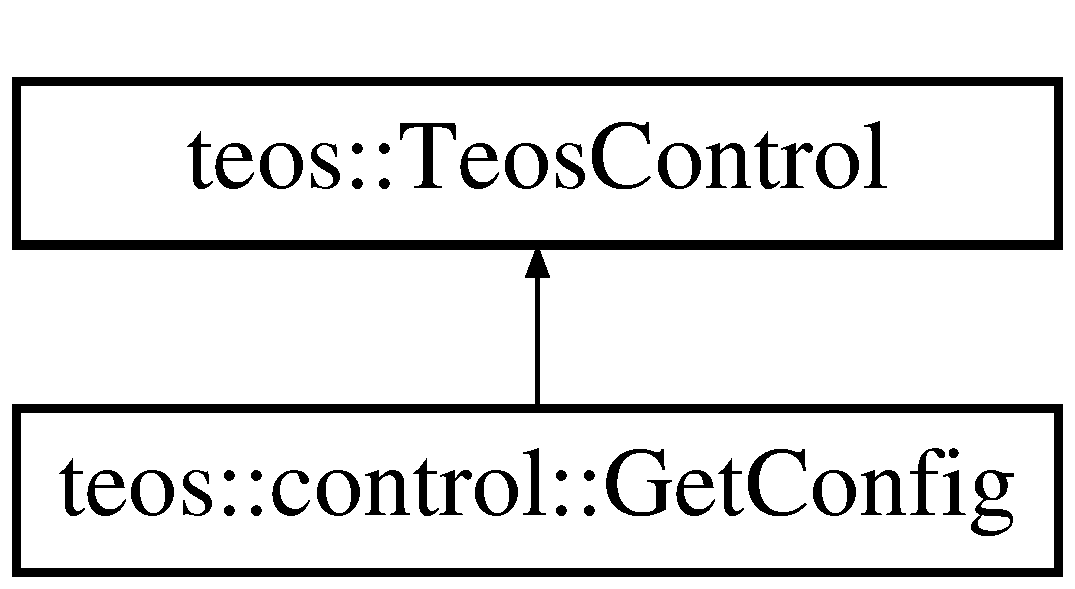
\includegraphics[height=2.000000cm]{classteos_1_1control_1_1_get_config}
\end{center}
\end{figure}
\subsection*{Additional Inherited Members}


The documentation for this class was generated from the following file\+:\begin{DoxyCompactItemize}
\item 
include/teoslib/control/config.\+hpp\end{DoxyCompactItemize}

\hypertarget{classteos_1_1control_1_1_get_config_options}{}\section{teos\+:\+:control\+:\+:Get\+Config\+Options Class Reference}
\label{classteos_1_1control_1_1_get_config_options}\index{teos\+::control\+::\+Get\+Config\+Options@{teos\+::control\+::\+Get\+Config\+Options}}
Inheritance diagram for teos\+:\+:control\+:\+:Get\+Config\+Options\+:\begin{figure}[H]
\begin{center}
\leavevmode
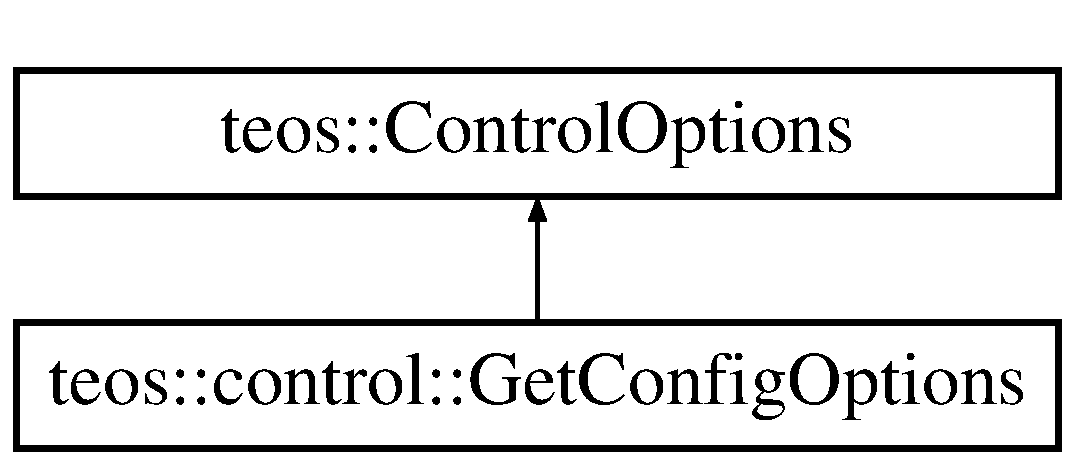
\includegraphics[height=2.000000cm]{classteos_1_1control_1_1_get_config_options}
\end{center}
\end{figure}
\subsection*{Public Member Functions}
\begin{DoxyCompactItemize}
\item 
\mbox{\Hypertarget{classteos_1_1control_1_1_get_config_options_ac0b1b2f54b11f08161adc68e5f8f6aa0}\label{classteos_1_1control_1_1_get_config_options_ac0b1b2f54b11f08161adc68e5f8f6aa0}} 
{\bfseries Get\+Config\+Options} (int argc, const char $\ast$$\ast$argv)
\end{DoxyCompactItemize}
\subsection*{Protected Member Functions}
\begin{DoxyCompactItemize}
\item 
const char $\ast$ \mbox{\hyperlink{classteos_1_1control_1_1_get_config_options_a144b88309b989f2282da43ad56ddb1a6}{get\+Usage}} ()
\begin{DoxyCompactList}\small\item\em Command \textquotesingle{}usage\textquotesingle{} instruction. \end{DoxyCompactList}\item 
\mbox{\Hypertarget{classteos_1_1control_1_1_get_config_options_a842924b3643e7830d15f567f89dfc4a2}\label{classteos_1_1control_1_1_get_config_options_a842924b3643e7830d15f567f89dfc4a2}} 
\mbox{\hyperlink{classteos_1_1_teos_control}{Teos\+Control}} {\bfseries execute\+Command} ()
\end{DoxyCompactItemize}
\subsection*{Additional Inherited Members}


\subsection{Member Function Documentation}
\mbox{\Hypertarget{classteos_1_1control_1_1_get_config_options_a144b88309b989f2282da43ad56ddb1a6}\label{classteos_1_1control_1_1_get_config_options_a144b88309b989f2282da43ad56ddb1a6}} 
\index{teos\+::control\+::\+Get\+Config\+Options@{teos\+::control\+::\+Get\+Config\+Options}!get\+Usage@{get\+Usage}}
\index{get\+Usage@{get\+Usage}!teos\+::control\+::\+Get\+Config\+Options@{teos\+::control\+::\+Get\+Config\+Options}}
\subsubsection{\texorpdfstring{get\+Usage()}{getUsage()}}
{\footnotesize\ttfamily const char$\ast$ teos\+::control\+::\+Get\+Config\+Options\+::get\+Usage (\begin{DoxyParamCaption}{ }\end{DoxyParamCaption})\hspace{0.3cm}{\ttfamily [inline]}, {\ttfamily [protected]}, {\ttfamily [virtual]}}



Command \textquotesingle{}usage\textquotesingle{} instruction. 

\begin{DoxyReturn}{Returns}
usage text 
\end{DoxyReturn}


Reimplemented from \mbox{\hyperlink{classteos_1_1_control_options_a0aa5671f9bc750ed5280c26c543874f3}{teos\+::\+Control\+Options}}.



The documentation for this class was generated from the following file\+:\begin{DoxyCompactItemize}
\item 
teos\+\_\+lib/include/teoslib/control/config.\+hpp\end{DoxyCompactItemize}

\hypertarget{classteos_1_1command_1_1_get_info}{}\section{teos\+:\+:command\+:\+:Get\+Info Class Reference}
\label{classteos_1_1command_1_1_get_info}\index{teos\+::command\+::\+Get\+Info@{teos\+::command\+::\+Get\+Info}}


Get current blockchain information.  




{\ttfamily \#include $<$get\+\_\+commands.\+hpp$>$}

Inheritance diagram for teos\+:\+:command\+:\+:Get\+Info\+:\begin{figure}[H]
\begin{center}
\leavevmode
\includegraphics[height=3.000000cm]{classteos_1_1command_1_1_get_info}
\end{center}
\end{figure}
\subsection*{Public Member Functions}
\begin{DoxyCompactItemize}
\item 
\mbox{\Hypertarget{classteos_1_1command_1_1_get_info_ac15b485dd53c3b440a09bdb2be5bbc27}\label{classteos_1_1command_1_1_get_info_ac15b485dd53c3b440a09bdb2be5bbc27}} 
{\bfseries Get\+Info} (bool raw=false)
\item 
\mbox{\Hypertarget{classteos_1_1command_1_1_get_info_ac12a0c7b894af0d486737d299c776244}\label{classteos_1_1command_1_1_get_info_ac12a0c7b894af0d486737d299c776244}} 
{\bfseries Get\+Info} (ptree req\+Json, bool raw=false)
\end{DoxyCompactItemize}
\subsection*{Additional Inherited Members}


\subsection{Detailed Description}
Get current blockchain information. 

The documentation for this class was generated from the following file\+:\begin{DoxyCompactItemize}
\item 
teos\+\_\+lib/include/teoslib/command/\mbox{\hyperlink{get__commands_8hpp}{get\+\_\+commands.\+hpp}}\end{DoxyCompactItemize}

\hypertarget{classteos_1_1command_1_1_get_info_options}{}\section{teos\+:\+:command\+:\+:Get\+Info\+Options Class Reference}
\label{classteos_1_1command_1_1_get_info_options}\index{teos\+::command\+::\+Get\+Info\+Options@{teos\+::command\+::\+Get\+Info\+Options}}


Command-\/line driver for the \mbox{\hyperlink{classteos_1_1command_1_1_get_info}{Get\+Info}} class.  




{\ttfamily \#include $<$get\+\_\+commands.\+hpp$>$}

Inheritance diagram for teos\+:\+:command\+:\+:Get\+Info\+Options\+:\begin{figure}[H]
\begin{center}
\leavevmode
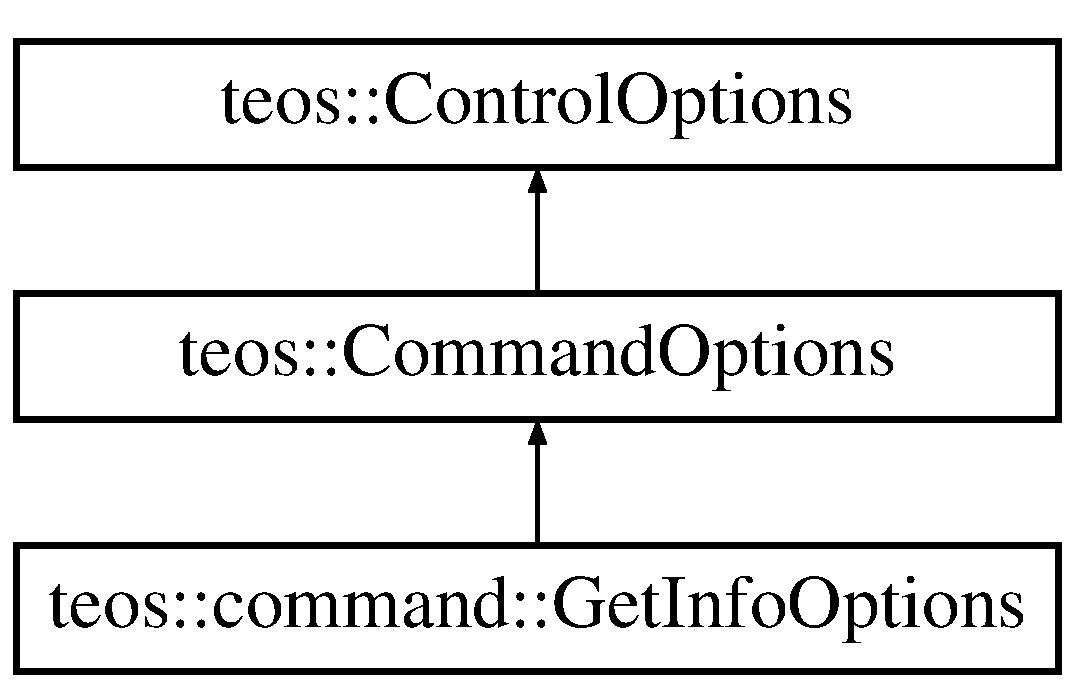
\includegraphics[height=3.000000cm]{classteos_1_1command_1_1_get_info_options}
\end{center}
\end{figure}
\subsection*{Public Member Functions}
\begin{DoxyCompactItemize}
\item 
\mbox{\Hypertarget{classteos_1_1command_1_1_get_info_options_a4d4b80ca0552b6dc743103af36f5746a}\label{classteos_1_1command_1_1_get_info_options_a4d4b80ca0552b6dc743103af36f5746a}} 
{\bfseries Get\+Info\+Options} (int argc, const char $\ast$$\ast$argv)
\end{DoxyCompactItemize}
\subsection*{Protected Member Functions}
\begin{DoxyCompactItemize}
\item 
const char $\ast$ \mbox{\hyperlink{classteos_1_1command_1_1_get_info_options_af5b6ec0a42f019ef1058e6f78a84346d}{get\+Usage}} ()
\begin{DoxyCompactList}\small\item\em Command \textquotesingle{}usage\textquotesingle{} instruction. \end{DoxyCompactList}\item 
\mbox{\Hypertarget{classteos_1_1command_1_1_get_info_options_a34618d24dee722d76c13da4d2010fd63}\label{classteos_1_1command_1_1_get_info_options_a34618d24dee722d76c13da4d2010fd63}} 
\mbox{\hyperlink{classteos_1_1_teos_control}{Teos\+Control}} {\bfseries execute\+Command} ()
\item 
\mbox{\Hypertarget{classteos_1_1command_1_1_get_info_options_a2713f566133468d9d576e71bd3471f6d}\label{classteos_1_1command_1_1_get_info_options_a2713f566133468d9d576e71bd3471f6d}} 
void {\bfseries printout} (\mbox{\hyperlink{classteos_1_1_teos_control}{Teos\+Control}} command, variables\+\_\+map \&vm)
\end{DoxyCompactItemize}
\subsection*{Additional Inherited Members}


\subsection{Detailed Description}
Command-\/line driver for the \mbox{\hyperlink{classteos_1_1command_1_1_get_info}{Get\+Info}} class. 

\subsection{Member Function Documentation}
\mbox{\Hypertarget{classteos_1_1command_1_1_get_info_options_af5b6ec0a42f019ef1058e6f78a84346d}\label{classteos_1_1command_1_1_get_info_options_af5b6ec0a42f019ef1058e6f78a84346d}} 
\index{teos\+::command\+::\+Get\+Info\+Options@{teos\+::command\+::\+Get\+Info\+Options}!get\+Usage@{get\+Usage}}
\index{get\+Usage@{get\+Usage}!teos\+::command\+::\+Get\+Info\+Options@{teos\+::command\+::\+Get\+Info\+Options}}
\subsubsection{\texorpdfstring{get\+Usage()}{getUsage()}}
{\footnotesize\ttfamily const char$\ast$ teos\+::command\+::\+Get\+Info\+Options\+::get\+Usage (\begin{DoxyParamCaption}{ }\end{DoxyParamCaption})\hspace{0.3cm}{\ttfamily [inline]}, {\ttfamily [protected]}, {\ttfamily [virtual]}}



Command \textquotesingle{}usage\textquotesingle{} instruction. 

\begin{DoxyReturn}{Returns}
usage text 
\end{DoxyReturn}


Reimplemented from \mbox{\hyperlink{classteos_1_1_control_options_a0aa5671f9bc750ed5280c26c543874f3}{teos\+::\+Control\+Options}}.



The documentation for this class was generated from the following file\+:\begin{DoxyCompactItemize}
\item 
include/teoslib/command/\mbox{\hyperlink{get__commands_8hpp}{get\+\_\+commands.\+hpp}}\end{DoxyCompactItemize}

\hypertarget{classteos_1_1command_1_1_get_table}{}\section{teos\+:\+:command\+:\+:Get\+Table Class Reference}
\label{classteos_1_1command_1_1_get_table}\index{teos\+::command\+::\+Get\+Table@{teos\+::command\+::\+Get\+Table}}


Retrieves the contents of a database table.  




{\ttfamily \#include $<$get\+\_\+commands.\+hpp$>$}

Inheritance diagram for teos\+:\+:command\+:\+:Get\+Table\+:\begin{figure}[H]
\begin{center}
\leavevmode
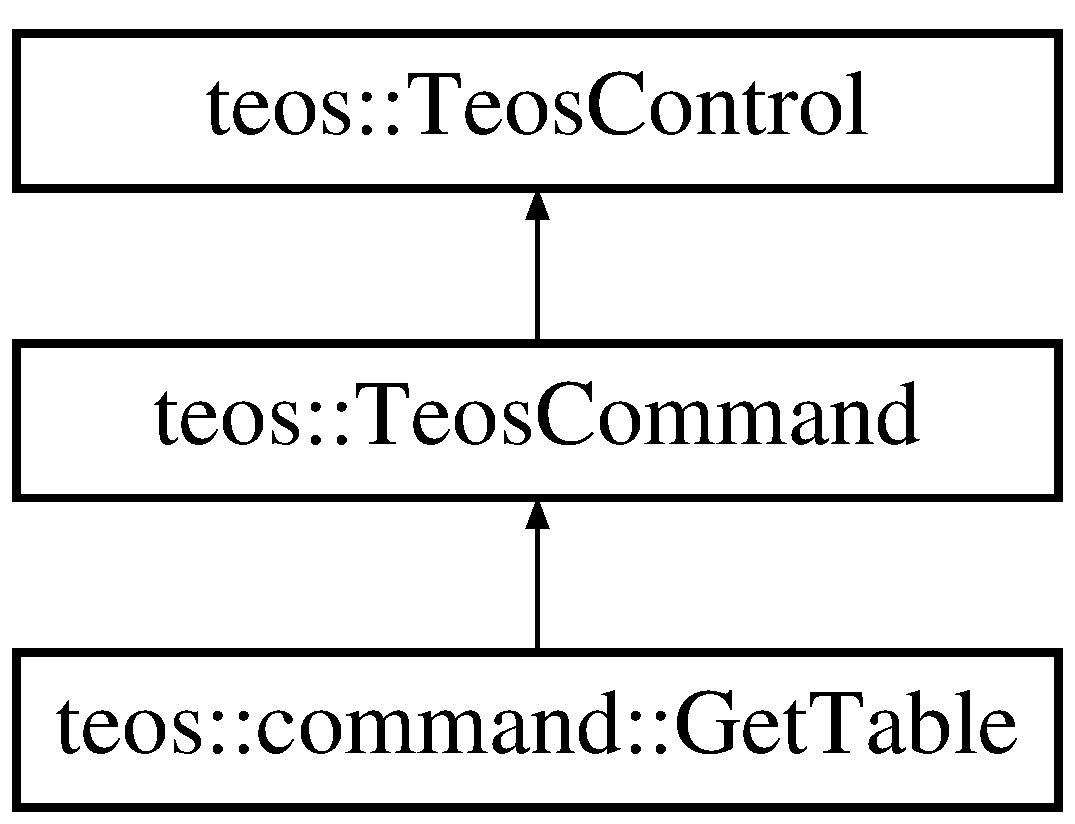
\includegraphics[height=3.000000cm]{classteos_1_1command_1_1_get_table}
\end{center}
\end{figure}
\subsection*{Public Member Functions}
\begin{DoxyCompactItemize}
\item 
\mbox{\Hypertarget{classteos_1_1command_1_1_get_table_a8b928495589a3ce8b24852bb814869a6}\label{classteos_1_1command_1_1_get_table_a8b928495589a3ce8b24852bb814869a6}} 
{\bfseries Get\+Table} (string contract, string scope, string table, unsigned limit=10, string key=\char`\"{}\char`\"{}, string lower=\char`\"{}\char`\"{}, string upper=\char`\"{}\char`\"{})
\item 
\mbox{\Hypertarget{classteos_1_1command_1_1_get_table_a528f99f802b4406e9d87692d5d7946a5}\label{classteos_1_1command_1_1_get_table_a528f99f802b4406e9d87692d5d7946a5}} 
{\bfseries Get\+Table} (ptree req\+Json, bool raw=false)
\item 
\mbox{\Hypertarget{classteos_1_1command_1_1_get_table_a1ef3e9835bf66ba7dcc86f4899e4dba4}\label{classteos_1_1command_1_1_get_table_a1ef3e9835bf66ba7dcc86f4899e4dba4}} 
string {\bfseries norm\+Request} (ptree \&req\+Json)
\end{DoxyCompactItemize}
\subsection*{Additional Inherited Members}


\subsection{Detailed Description}
Retrieves the contents of a database table. 

The documentation for this class was generated from the following file\+:\begin{DoxyCompactItemize}
\item 
teos\+\_\+lib/include/teoslib/command/\mbox{\hyperlink{get__commands_8hpp}{get\+\_\+commands.\+hpp}}\end{DoxyCompactItemize}

\hypertarget{classteos_1_1command_1_1_get_table_options}{}\section{teos\+:\+:command\+:\+:Get\+Table\+Options Class Reference}
\label{classteos_1_1command_1_1_get_table_options}\index{teos\+::command\+::\+Get\+Table\+Options@{teos\+::command\+::\+Get\+Table\+Options}}
Inheritance diagram for teos\+:\+:command\+:\+:Get\+Table\+Options\+:\begin{figure}[H]
\begin{center}
\leavevmode
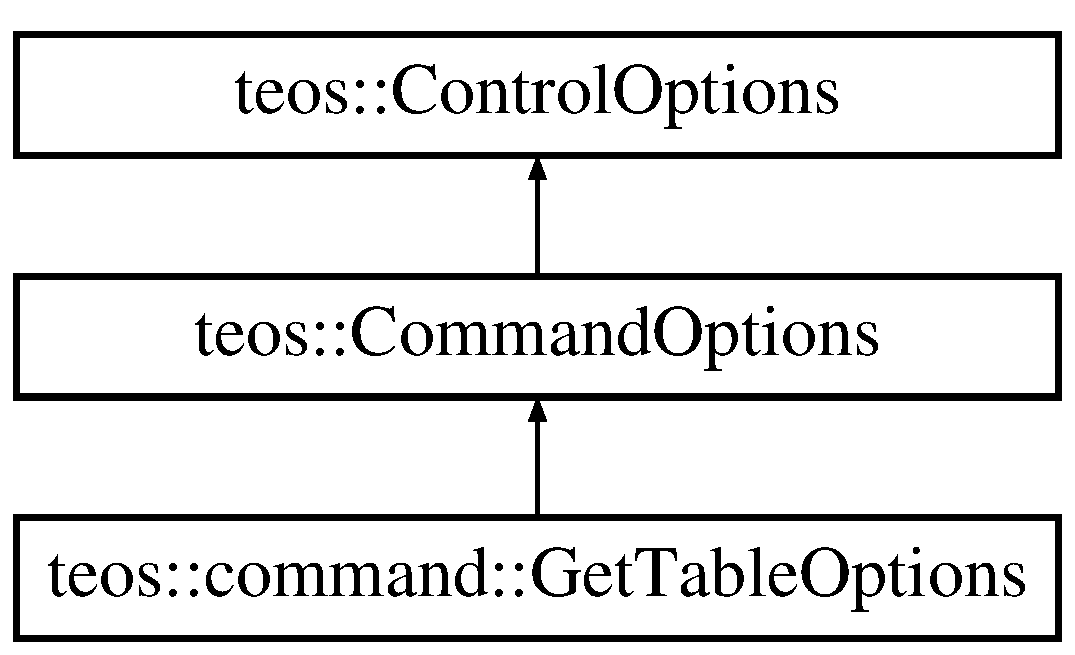
\includegraphics[height=3.000000cm]{classteos_1_1command_1_1_get_table_options}
\end{center}
\end{figure}
\subsection*{Public Member Functions}
\begin{DoxyCompactItemize}
\item 
\mbox{\Hypertarget{classteos_1_1command_1_1_get_table_options_a36eaf178fdb3962791587e24eaa0e1b9}\label{classteos_1_1command_1_1_get_table_options_a36eaf178fdb3962791587e24eaa0e1b9}} 
{\bfseries Get\+Table\+Options} (int argc, const char $\ast$$\ast$argv)
\end{DoxyCompactItemize}
\subsection*{Protected Member Functions}
\begin{DoxyCompactItemize}
\item 
const char $\ast$ \mbox{\hyperlink{classteos_1_1command_1_1_get_table_options_a764b61a7d83e508673b73100c45c3d13}{get\+Usage}} ()
\begin{DoxyCompactList}\small\item\em Command \textquotesingle{}usage\textquotesingle{} instruction. \end{DoxyCompactList}\item 
\mbox{\Hypertarget{classteos_1_1command_1_1_get_table_options_a35a7ee5c807bf244c3ecb959f93f2f74}\label{classteos_1_1command_1_1_get_table_options_a35a7ee5c807bf244c3ecb959f93f2f74}} 
options\+\_\+description {\bfseries argument\+Description} ()
\item 
\mbox{\Hypertarget{classteos_1_1command_1_1_get_table_options_a2b6533c23e19f02dbcb1e942bec667b5}\label{classteos_1_1command_1_1_get_table_options_a2b6533c23e19f02dbcb1e942bec667b5}} 
void {\bfseries set\+Pos\+Desc} (positional\+\_\+options\+\_\+description \&pos\+\_\+desc)
\item 
\mbox{\Hypertarget{classteos_1_1command_1_1_get_table_options_a89b799411002a56db84efdada9c8d203}\label{classteos_1_1command_1_1_get_table_options_a89b799411002a56db84efdada9c8d203}} 
bool {\bfseries check\+Arguments} (variables\+\_\+map \&vm)
\item 
\mbox{\Hypertarget{classteos_1_1command_1_1_get_table_options_a38ec528365a160cef25ceeba6e0cbfca}\label{classteos_1_1command_1_1_get_table_options_a38ec528365a160cef25ceeba6e0cbfca}} 
\mbox{\hyperlink{classteos_1_1_teos_control}{Teos\+Control}} {\bfseries execute\+Command} ()
\end{DoxyCompactItemize}
\subsection*{Protected Attributes}
\begin{DoxyCompactItemize}
\item 
\mbox{\Hypertarget{classteos_1_1command_1_1_get_table_options_a70e8e164df0b518f1147da98680e33b8}\label{classteos_1_1command_1_1_get_table_options_a70e8e164df0b518f1147da98680e33b8}} 
string {\bfseries contract}
\item 
\mbox{\Hypertarget{classteos_1_1command_1_1_get_table_options_a5895ffd2367c60345c0ea9b18c1f97f1}\label{classteos_1_1command_1_1_get_table_options_a5895ffd2367c60345c0ea9b18c1f97f1}} 
string {\bfseries scope}
\item 
\mbox{\Hypertarget{classteos_1_1command_1_1_get_table_options_a1ffe2c0a4aa1ef8e550616f36ebd14e2}\label{classteos_1_1command_1_1_get_table_options_a1ffe2c0a4aa1ef8e550616f36ebd14e2}} 
string {\bfseries table}
\item 
\mbox{\Hypertarget{classteos_1_1command_1_1_get_table_options_af8450a13304574151c9cb8787a174614}\label{classteos_1_1command_1_1_get_table_options_af8450a13304574151c9cb8787a174614}} 
unsigned {\bfseries limit}
\item 
\mbox{\Hypertarget{classteos_1_1command_1_1_get_table_options_a3070c3e6665a0ec03e637f315e9d17b0}\label{classteos_1_1command_1_1_get_table_options_a3070c3e6665a0ec03e637f315e9d17b0}} 
string {\bfseries key}
\item 
\mbox{\Hypertarget{classteos_1_1command_1_1_get_table_options_a3b19da7686f7c93abbba4dd0b0690f17}\label{classteos_1_1command_1_1_get_table_options_a3b19da7686f7c93abbba4dd0b0690f17}} 
string {\bfseries lower}
\item 
\mbox{\Hypertarget{classteos_1_1command_1_1_get_table_options_a98f3e59e470bd182e9c1036eea94fd79}\label{classteos_1_1command_1_1_get_table_options_a98f3e59e470bd182e9c1036eea94fd79}} 
string {\bfseries upper}
\end{DoxyCompactItemize}
\subsection*{Additional Inherited Members}


\subsection{Member Function Documentation}
\mbox{\Hypertarget{classteos_1_1command_1_1_get_table_options_a764b61a7d83e508673b73100c45c3d13}\label{classteos_1_1command_1_1_get_table_options_a764b61a7d83e508673b73100c45c3d13}} 
\index{teos\+::command\+::\+Get\+Table\+Options@{teos\+::command\+::\+Get\+Table\+Options}!get\+Usage@{get\+Usage}}
\index{get\+Usage@{get\+Usage}!teos\+::command\+::\+Get\+Table\+Options@{teos\+::command\+::\+Get\+Table\+Options}}
\subsubsection{\texorpdfstring{get\+Usage()}{getUsage()}}
{\footnotesize\ttfamily const char$\ast$ teos\+::command\+::\+Get\+Table\+Options\+::get\+Usage (\begin{DoxyParamCaption}{ }\end{DoxyParamCaption})\hspace{0.3cm}{\ttfamily [inline]}, {\ttfamily [protected]}, {\ttfamily [virtual]}}



Command \textquotesingle{}usage\textquotesingle{} instruction. 

\begin{DoxyReturn}{Returns}
usage text 
\end{DoxyReturn}


Reimplemented from \mbox{\hyperlink{classteos_1_1_control_options_a0aa5671f9bc750ed5280c26c543874f3}{teos\+::\+Control\+Options}}.



The documentation for this class was generated from the following file\+:\begin{DoxyCompactItemize}
\item 
include/teoslib/command/\mbox{\hyperlink{get__commands_8hpp}{get\+\_\+commands.\+hpp}}\end{DoxyCompactItemize}

\hypertarget{structteos_1_1_init_get_json}{}\section{teos\+:\+:Init\+Get\+Json Struct Reference}
\label{structteos_1_1_init_get_json}\index{teos\+::\+Init\+Get\+Json@{teos\+::\+Init\+Get\+Json}}
\subsection*{Public Attributes}
\begin{DoxyCompactItemize}
\item 
\mbox{\Hypertarget{structteos_1_1_init_get_json_ae52964bccbe6d0f23f0e01586a8855b9}\label{structteos_1_1_init_get_json_ae52964bccbe6d0f23f0e01586a8855b9}} 
string {\bfseries str\+Val}
\item 
\mbox{\Hypertarget{structteos_1_1_init_get_json_ae86e224b84a021705317a0cf3e788f1f}\label{structteos_1_1_init_get_json_ae86e224b84a021705317a0cf3e788f1f}} 
int {\bfseries int\+Val}
\item 
\mbox{\Hypertarget{structteos_1_1_init_get_json_a30a13c796a6829e1b9ec711519012d64}\label{structteos_1_1_init_get_json_a30a13c796a6829e1b9ec711519012d64}} 
float {\bfseries float\+Val}
\item 
\mbox{\Hypertarget{structteos_1_1_init_get_json_a01c32cb0438e072c44cf5206ef0075d0}\label{structteos_1_1_init_get_json_a01c32cb0438e072c44cf5206ef0075d0}} 
boost\+::posix\+\_\+time\+::ptime {\bfseries ptime}
\end{DoxyCompactItemize}


The documentation for this struct was generated from the following file\+:\begin{DoxyCompactItemize}
\item 
teos\+\_\+lib/utilities.\+cpp\end{DoxyCompactItemize}

\hypertarget{classteos_1_1command_1_1_key_pair}{}\section{teos\+:\+:command\+:\+:Key\+Pair Class Reference}
\label{classteos_1_1command_1_1_key_pair}\index{teos\+::command\+::\+Key\+Pair@{teos\+::command\+::\+Key\+Pair}}
\subsection*{Static Public Member Functions}
\begin{DoxyCompactItemize}
\item 
\mbox{\Hypertarget{classteos_1_1command_1_1_key_pair_a296e5566e03dd649860c3ef98e152682}\label{classteos_1_1command_1_1_key_pair_a296e5566e03dd649860c3ef98e152682}} 
static string {\bfseries privateK} ()
\end{DoxyCompactItemize}
\subsection*{Public Attributes}
\begin{DoxyCompactItemize}
\item 
\mbox{\Hypertarget{classteos_1_1command_1_1_key_pair_a6f255ea2d4ebc95b7af0da0ae9fb4618}\label{classteos_1_1command_1_1_key_pair_a6f255ea2d4ebc95b7af0da0ae9fb4618}} 
string {\bfseries private\+Key}
\item 
\mbox{\Hypertarget{classteos_1_1command_1_1_key_pair_a642b4737875a24960d8acfd27f6bccc7}\label{classteos_1_1command_1_1_key_pair_a642b4737875a24960d8acfd27f6bccc7}} 
string {\bfseries public\+Key}
\end{DoxyCompactItemize}
\subsection*{Static Public Attributes}
\begin{DoxyCompactItemize}
\item 
\mbox{\Hypertarget{classteos_1_1command_1_1_key_pair_accd00dfb50854f396732befecdcf71d1}\label{classteos_1_1command_1_1_key_pair_accd00dfb50854f396732befecdcf71d1}} 
static string {\bfseries prk} = Key\+Pair\+::privateK()
\end{DoxyCompactItemize}


The documentation for this class was generated from the following files\+:\begin{DoxyCompactItemize}
\item 
teos\+\_\+lib/include/teoslib/eos\+\_\+interface.\+hpp\item 
teos\+\_\+lib/eos\+\_\+interface.\+cpp\end{DoxyCompactItemize}

\hypertarget{classteos_1_1command_1_1_push_action}{}\section{teos\+:\+:command\+:\+:Push\+Action Class Reference}
\label{classteos_1_1command_1_1_push_action}\index{teos\+::command\+::\+Push\+Action@{teos\+::command\+::\+Push\+Action}}


{\ttfamily \#include $<$push\+\_\+commands.\+hpp$>$}

Inheritance diagram for teos\+:\+:command\+:\+:Push\+Action\+:\begin{figure}[H]
\begin{center}
\leavevmode
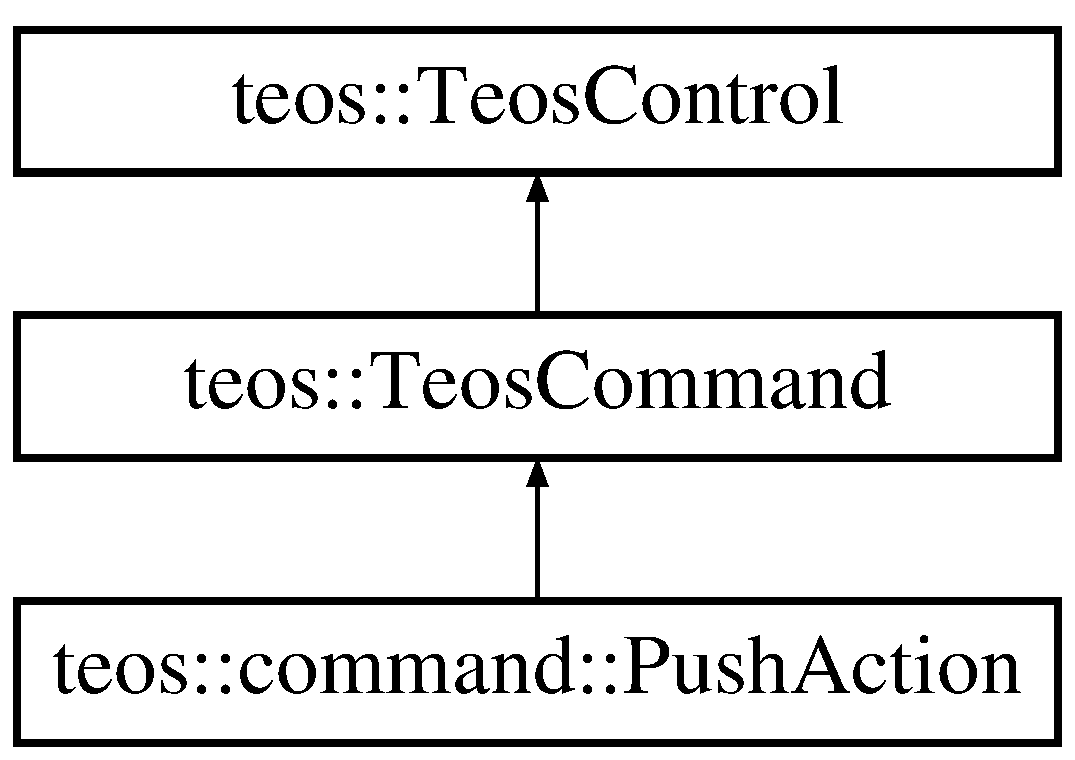
\includegraphics[height=3.000000cm]{classteos_1_1command_1_1_push_action}
\end{center}
\end{figure}
\subsection*{Public Member Functions}
\begin{DoxyCompactItemize}
\item 
\mbox{\Hypertarget{classteos_1_1command_1_1_push_action_a97565647ccfdf55a8e0e5a6d2ed25d32}\label{classteos_1_1command_1_1_push_action_a97565647ccfdf55a8e0e5a6d2ed25d32}} 
{\bfseries Push\+Action} (string contract\+Name, string action, string data, string permission=\char`\"{}\char`\"{}, unsigned expiration\+Sec=30, bool skip\+Signature=false, bool dont\+Broadcast=false, bool force\+Unique=false, unsigned max\+Cpu\+Usage=0, unsigned max\+Net\+Usage=0)
\item 
\mbox{\Hypertarget{classteos_1_1command_1_1_push_action_a8bca4e4fa0586c2d2242a3a50e25cc07}\label{classteos_1_1command_1_1_push_action_a8bca4e4fa0586c2d2242a3a50e25cc07}} 
{\bfseries Push\+Action} (ptree req\+Json)
\end{DoxyCompactItemize}
\subsection*{Additional Inherited Members}


\subsection{Detailed Description}
Push a transaction with a single message 

The documentation for this class was generated from the following file\+:\begin{DoxyCompactItemize}
\item 
include/teoslib/command/push\+\_\+commands.\+hpp\end{DoxyCompactItemize}

\hypertarget{classteos_1_1command_1_1_push_action_options}{}\section{teos\+:\+:command\+:\+:Push\+Action\+Options Class Reference}
\label{classteos_1_1command_1_1_push_action_options}\index{teos\+::command\+::\+Push\+Action\+Options@{teos\+::command\+::\+Push\+Action\+Options}}


Command-\/line driver for the \mbox{\hyperlink{classteos_1_1command_1_1_push_action}{Push\+Action}} class.  




{\ttfamily \#include $<$push\+\_\+commands.\+hpp$>$}

Inheritance diagram for teos\+:\+:command\+:\+:Push\+Action\+Options\+:\begin{figure}[H]
\begin{center}
\leavevmode
\includegraphics[height=3.000000cm]{classteos_1_1command_1_1_push_action_options}
\end{center}
\end{figure}
\subsection*{Public Member Functions}
\begin{DoxyCompactItemize}
\item 
\mbox{\Hypertarget{classteos_1_1command_1_1_push_action_options_a3bb2cab6e95fe807a16f62dac7252664}\label{classteos_1_1command_1_1_push_action_options_a3bb2cab6e95fe807a16f62dac7252664}} 
{\bfseries Push\+Action\+Options} (int argc, const char $\ast$$\ast$argv)
\end{DoxyCompactItemize}
\subsection*{Protected Member Functions}
\begin{DoxyCompactItemize}
\item 
const char $\ast$ \mbox{\hyperlink{classteos_1_1command_1_1_push_action_options_a1dac78e7b40cc0ff91895d1fc0f7d2b4}{get\+Usage}} ()
\begin{DoxyCompactList}\small\item\em Command \textquotesingle{}usage\textquotesingle{} instruction. \end{DoxyCompactList}\item 
\mbox{\Hypertarget{classteos_1_1command_1_1_push_action_options_a1d7e797f32e83b014a38d8a209e957e9}\label{classteos_1_1command_1_1_push_action_options_a1d7e797f32e83b014a38d8a209e957e9}} 
options\+\_\+description {\bfseries argument\+Description} ()
\item 
\mbox{\Hypertarget{classteos_1_1command_1_1_push_action_options_a1e3278dc5640f50a32a9965121eba36d}\label{classteos_1_1command_1_1_push_action_options_a1e3278dc5640f50a32a9965121eba36d}} 
void {\bfseries set\+Pos\+Desc} (positional\+\_\+options\+\_\+description \&pos\+\_\+desc)
\item 
\mbox{\Hypertarget{classteos_1_1command_1_1_push_action_options_a48ff4a653e24e3322641a64063dbf340}\label{classteos_1_1command_1_1_push_action_options_a48ff4a653e24e3322641a64063dbf340}} 
bool {\bfseries check\+Arguments} (variables\+\_\+map \&vm)
\item 
\mbox{\Hypertarget{classteos_1_1command_1_1_push_action_options_a2f8c261e50aca98cdf61a6cd44b48656}\label{classteos_1_1command_1_1_push_action_options_a2f8c261e50aca98cdf61a6cd44b48656}} 
\mbox{\hyperlink{classteos_1_1_teos_control}{Teos\+Control}} {\bfseries execute\+Command} ()
\item 
\mbox{\Hypertarget{classteos_1_1command_1_1_push_action_options_af073d742bdb1d32f12344a6ee305ff83}\label{classteos_1_1command_1_1_push_action_options_af073d742bdb1d32f12344a6ee305ff83}} 
void {\bfseries printout} (\mbox{\hyperlink{classteos_1_1_teos_control}{Teos\+Control}} command, variables\+\_\+map \&vm)
\end{DoxyCompactItemize}
\subsection*{Protected Attributes}
\begin{DoxyCompactItemize}
\item 
\mbox{\Hypertarget{classteos_1_1command_1_1_push_action_options_a4a76bcabc3ac3cf6c66681c9f9ebb220}\label{classteos_1_1command_1_1_push_action_options_a4a76bcabc3ac3cf6c66681c9f9ebb220}} 
string {\bfseries contract}
\item 
\mbox{\Hypertarget{classteos_1_1command_1_1_push_action_options_a294978a4531e49026f2e7f5cce370ad5}\label{classteos_1_1command_1_1_push_action_options_a294978a4531e49026f2e7f5cce370ad5}} 
string {\bfseries action}
\item 
\mbox{\Hypertarget{classteos_1_1command_1_1_push_action_options_a7175cf75c17f7b51d723d9384a09c216}\label{classteos_1_1command_1_1_push_action_options_a7175cf75c17f7b51d723d9384a09c216}} 
string {\bfseries data}
\item 
\mbox{\Hypertarget{classteos_1_1command_1_1_push_action_options_a697eabe0ad96c3935f4827a2cae5c713}\label{classteos_1_1command_1_1_push_action_options_a697eabe0ad96c3935f4827a2cae5c713}} 
string {\bfseries permission}
\item 
\mbox{\Hypertarget{classteos_1_1command_1_1_push_action_options_adf7dd2d0a13d799bb866bc84743d374d}\label{classteos_1_1command_1_1_push_action_options_adf7dd2d0a13d799bb866bc84743d374d}} 
unsigned {\bfseries expiration}
\item 
\mbox{\Hypertarget{classteos_1_1command_1_1_push_action_options_ab99e9a1172b0c190fb73edef354ed4a9}\label{classteos_1_1command_1_1_push_action_options_ab99e9a1172b0c190fb73edef354ed4a9}} 
bool {\bfseries skip\+Signature}
\item 
\mbox{\Hypertarget{classteos_1_1command_1_1_push_action_options_abff73f229e198e0a651fd0451ddc57d1}\label{classteos_1_1command_1_1_push_action_options_abff73f229e198e0a651fd0451ddc57d1}} 
bool {\bfseries dont\+Broadcast}
\item 
\mbox{\Hypertarget{classteos_1_1command_1_1_push_action_options_a27d78056bb82d50ac5bdcaaf4404dd92}\label{classteos_1_1command_1_1_push_action_options_a27d78056bb82d50ac5bdcaaf4404dd92}} 
bool {\bfseries force\+Unique}
\item 
\mbox{\Hypertarget{classteos_1_1command_1_1_push_action_options_a933a3a5d4d21d34bb561d16dcf61cf65}\label{classteos_1_1command_1_1_push_action_options_a933a3a5d4d21d34bb561d16dcf61cf65}} 
unsigned {\bfseries max\+Cpu\+Usage}
\item 
\mbox{\Hypertarget{classteos_1_1command_1_1_push_action_options_ad6e5bcfc6ec47f87bfd7a03efd87f629}\label{classteos_1_1command_1_1_push_action_options_ad6e5bcfc6ec47f87bfd7a03efd87f629}} 
unsigned {\bfseries max\+Net\+Usage}
\end{DoxyCompactItemize}
\subsection*{Additional Inherited Members}


\subsection{Detailed Description}
Command-\/line driver for the \mbox{\hyperlink{classteos_1_1command_1_1_push_action}{Push\+Action}} class. 

\subsection{Member Function Documentation}
\mbox{\Hypertarget{classteos_1_1command_1_1_push_action_options_a1dac78e7b40cc0ff91895d1fc0f7d2b4}\label{classteos_1_1command_1_1_push_action_options_a1dac78e7b40cc0ff91895d1fc0f7d2b4}} 
\index{teos\+::command\+::\+Push\+Action\+Options@{teos\+::command\+::\+Push\+Action\+Options}!get\+Usage@{get\+Usage}}
\index{get\+Usage@{get\+Usage}!teos\+::command\+::\+Push\+Action\+Options@{teos\+::command\+::\+Push\+Action\+Options}}
\subsubsection{\texorpdfstring{get\+Usage()}{getUsage()}}
{\footnotesize\ttfamily const char$\ast$ teos\+::command\+::\+Push\+Action\+Options\+::get\+Usage (\begin{DoxyParamCaption}{ }\end{DoxyParamCaption})\hspace{0.3cm}{\ttfamily [inline]}, {\ttfamily [protected]}, {\ttfamily [virtual]}}



Command \textquotesingle{}usage\textquotesingle{} instruction. 

\begin{DoxyReturn}{Returns}
usage text 
\end{DoxyReturn}


Reimplemented from \mbox{\hyperlink{classteos_1_1_control_options_a0aa5671f9bc750ed5280c26c543874f3}{teos\+::\+Control\+Options}}.



The documentation for this class was generated from the following file\+:\begin{DoxyCompactItemize}
\item 
include/teoslib/command/push\+\_\+commands.\+hpp\end{DoxyCompactItemize}

\hypertarget{classserver}{}\section{server Class Reference}
\label{classserver}\index{server@{server}}
\subsection*{Public Member Functions}
\begin{DoxyCompactItemize}
\item 
\mbox{\Hypertarget{classserver_add3cc1b2c469ccade459882d335e369f}\label{classserver_add3cc1b2c469ccade459882d335e369f}} 
{\bfseries server} (boost\+::asio\+::io\+\_\+service \&io\+\_\+service, short port)
\end{DoxyCompactItemize}


The documentation for this class was generated from the following file\+:\begin{DoxyCompactItemize}
\item 
asyntcpechoserver.\+cpp\end{DoxyCompactItemize}

\hypertarget{classsession}{}\section{session Class Reference}
\label{classsession}\index{session@{session}}
\subsection*{Public Member Functions}
\begin{DoxyCompactItemize}
\item 
\mbox{\Hypertarget{classsession_ae8ec671941d1b8c7ac1b54978692cc85}\label{classsession_ae8ec671941d1b8c7ac1b54978692cc85}} 
{\bfseries session} (boost\+::asio\+::io\+\_\+service \&io\+\_\+service)
\item 
\mbox{\Hypertarget{classsession_a877765bc7124ada6580ad2f748b4d72c}\label{classsession_a877765bc7124ada6580ad2f748b4d72c}} 
tcp\+::socket \& {\bfseries socket} ()
\item 
\mbox{\Hypertarget{classsession_ad69144e27f558b8960efae132f2e15f4}\label{classsession_ad69144e27f558b8960efae132f2e15f4}} 
void {\bfseries start} ()
\end{DoxyCompactItemize}


The documentation for this class was generated from the following file\+:\begin{DoxyCompactItemize}
\item 
asyntcpechoserver.\+cpp\end{DoxyCompactItemize}

\hypertarget{classteos_1_1command_1_1_set_contract}{}\section{teos\+:\+:command\+:\+:Set\+Contract Class Reference}
\label{classteos_1_1command_1_1_set_contract}\index{teos\+::command\+::\+Set\+Contract@{teos\+::command\+::\+Set\+Contract}}


{\ttfamily \#include $<$set\+\_\+commands.\+hpp$>$}

Inheritance diagram for teos\+:\+:command\+:\+:Set\+Contract\+:\begin{figure}[H]
\begin{center}
\leavevmode
\includegraphics[height=3.000000cm]{classteos_1_1command_1_1_set_contract}
\end{center}
\end{figure}
\subsection*{Public Member Functions}
\begin{DoxyCompactItemize}
\item 
\mbox{\Hypertarget{classteos_1_1command_1_1_set_contract_a1a851280aa0011a523640ea79221d095}\label{classteos_1_1command_1_1_set_contract_a1a851280aa0011a523640ea79221d095}} 
{\bfseries Set\+Contract} (string account\+Name, string contract\+Dir, string wast\+File=\char`\"{}\char`\"{}, string abi\+File=\char`\"{}\char`\"{}, string permission=\char`\"{}\char`\"{}, unsigned expiration=30, bool skip\+Signature=false, bool dont\+Broadcast=false, bool force\+Unique=false, unsigned max\+Cpu\+Usage=0, unsigned max\+Net\+Usage=0)
\item 
\mbox{\Hypertarget{classteos_1_1command_1_1_set_contract_ad964aae40c3062bbb1a40fad503df852}\label{classteos_1_1command_1_1_set_contract_ad964aae40c3062bbb1a40fad503df852}} 
{\bfseries Set\+Contract} (ptree req\+Json)
\end{DoxyCompactItemize}
\subsection*{Additional Inherited Members}


\subsection{Detailed Description}
Create or update the contract on an account. 

The documentation for this class was generated from the following file\+:\begin{DoxyCompactItemize}
\item 
include/teoslib/command/set\+\_\+commands.\+hpp\end{DoxyCompactItemize}

\hypertarget{classteos_1_1command_1_1_set_contract_options}{}\section{teos\+:\+:command\+:\+:Set\+Contract\+Options Class Reference}
\label{classteos_1_1command_1_1_set_contract_options}\index{teos\+::command\+::\+Set\+Contract\+Options@{teos\+::command\+::\+Set\+Contract\+Options}}


Command-\/line driver for the \mbox{\hyperlink{classteos_1_1command_1_1_set_contract}{Set\+Contract}} class.  




{\ttfamily \#include $<$set\+\_\+commands.\+hpp$>$}

Inheritance diagram for teos\+:\+:command\+:\+:Set\+Contract\+Options\+:\begin{figure}[H]
\begin{center}
\leavevmode
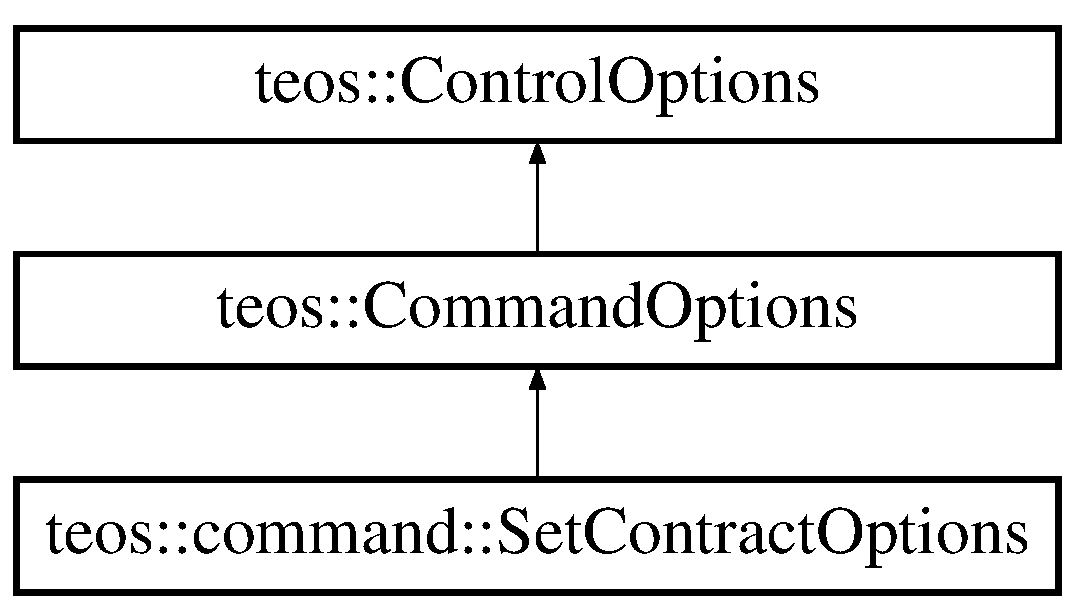
\includegraphics[height=3.000000cm]{classteos_1_1command_1_1_set_contract_options}
\end{center}
\end{figure}
\subsection*{Public Member Functions}
\begin{DoxyCompactItemize}
\item 
\mbox{\Hypertarget{classteos_1_1command_1_1_set_contract_options_af39ea067efeaafd5cc82211f86e7bbbe}\label{classteos_1_1command_1_1_set_contract_options_af39ea067efeaafd5cc82211f86e7bbbe}} 
{\bfseries Set\+Contract\+Options} (int argc, const char $\ast$$\ast$argv)
\end{DoxyCompactItemize}
\subsection*{Protected Member Functions}
\begin{DoxyCompactItemize}
\item 
const char $\ast$ \mbox{\hyperlink{classteos_1_1command_1_1_set_contract_options_a9176e2b58b222d45c975d6e9fa9b4ac7}{get\+Usage}} ()
\begin{DoxyCompactList}\small\item\em Command \textquotesingle{}usage\textquotesingle{} instruction. \end{DoxyCompactList}\item 
\mbox{\Hypertarget{classteos_1_1command_1_1_set_contract_options_a5115d6a5bc5a499e655556c44e014115}\label{classteos_1_1command_1_1_set_contract_options_a5115d6a5bc5a499e655556c44e014115}} 
options\+\_\+description {\bfseries argument\+Description} ()
\item 
\mbox{\Hypertarget{classteos_1_1command_1_1_set_contract_options_aadd7baa3b4b880ad65e079c10ef8a2a7}\label{classteos_1_1command_1_1_set_contract_options_aadd7baa3b4b880ad65e079c10ef8a2a7}} 
void {\bfseries set\+Pos\+Desc} (positional\+\_\+options\+\_\+description \&pos\+\_\+desc)
\item 
\mbox{\Hypertarget{classteos_1_1command_1_1_set_contract_options_ab735136b04248a943f121a564cc99c5e}\label{classteos_1_1command_1_1_set_contract_options_ab735136b04248a943f121a564cc99c5e}} 
bool {\bfseries check\+Arguments} (variables\+\_\+map \&vm)
\item 
\mbox{\Hypertarget{classteos_1_1command_1_1_set_contract_options_aa12f82f7deb7b77a994d1e1a92ea0eff}\label{classteos_1_1command_1_1_set_contract_options_aa12f82f7deb7b77a994d1e1a92ea0eff}} 
\mbox{\hyperlink{classteos_1_1_teos_control}{Teos\+Control}} {\bfseries execute\+Command} ()
\item 
\mbox{\Hypertarget{classteos_1_1command_1_1_set_contract_options_a85524966978c712794976f56dc3bb1c8}\label{classteos_1_1command_1_1_set_contract_options_a85524966978c712794976f56dc3bb1c8}} 
void {\bfseries printout} (\mbox{\hyperlink{classteos_1_1_teos_control}{Teos\+Control}} command, variables\+\_\+map \&vm)
\end{DoxyCompactItemize}
\subsection*{Protected Attributes}
\begin{DoxyCompactItemize}
\item 
\mbox{\Hypertarget{classteos_1_1command_1_1_set_contract_options_a10f47048e15f422d88e51ca0f75f51d8}\label{classteos_1_1command_1_1_set_contract_options_a10f47048e15f422d88e51ca0f75f51d8}} 
string {\bfseries account}
\item 
\mbox{\Hypertarget{classteos_1_1command_1_1_set_contract_options_abe8aa276fac772a23a0181b7ed9ef9f6}\label{classteos_1_1command_1_1_set_contract_options_abe8aa276fac772a23a0181b7ed9ef9f6}} 
string {\bfseries contract\+Dir}
\item 
\mbox{\Hypertarget{classteos_1_1command_1_1_set_contract_options_a7dbccd972bc3c50da39eea80458259a8}\label{classteos_1_1command_1_1_set_contract_options_a7dbccd972bc3c50da39eea80458259a8}} 
string {\bfseries wast\+File}
\item 
\mbox{\Hypertarget{classteos_1_1command_1_1_set_contract_options_ae4c7a5748465f86498c199e27ad8125e}\label{classteos_1_1command_1_1_set_contract_options_ae4c7a5748465f86498c199e27ad8125e}} 
string {\bfseries abi\+File}
\item 
\mbox{\Hypertarget{classteos_1_1command_1_1_set_contract_options_abe931527bc16569e549b955e9c303a6a}\label{classteos_1_1command_1_1_set_contract_options_abe931527bc16569e549b955e9c303a6a}} 
string {\bfseries permission}
\item 
\mbox{\Hypertarget{classteos_1_1command_1_1_set_contract_options_a12509c83b5e5fe824da0b8f9078040a9}\label{classteos_1_1command_1_1_set_contract_options_a12509c83b5e5fe824da0b8f9078040a9}} 
unsigned {\bfseries expiration}
\item 
\mbox{\Hypertarget{classteos_1_1command_1_1_set_contract_options_acf0d99696a5d73bb704a040bd11f1124}\label{classteos_1_1command_1_1_set_contract_options_acf0d99696a5d73bb704a040bd11f1124}} 
bool {\bfseries skip\+Signature}
\item 
\mbox{\Hypertarget{classteos_1_1command_1_1_set_contract_options_a7fcdae205dfbeb56cd891365017a3017}\label{classteos_1_1command_1_1_set_contract_options_a7fcdae205dfbeb56cd891365017a3017}} 
bool {\bfseries dont\+Broadcast}
\item 
\mbox{\Hypertarget{classteos_1_1command_1_1_set_contract_options_a9ec41b9060f09d5da9fe765bf698d8a2}\label{classteos_1_1command_1_1_set_contract_options_a9ec41b9060f09d5da9fe765bf698d8a2}} 
bool {\bfseries force\+Unique}
\item 
\mbox{\Hypertarget{classteos_1_1command_1_1_set_contract_options_a787f97b02b420867794f8a8f241fe48b}\label{classteos_1_1command_1_1_set_contract_options_a787f97b02b420867794f8a8f241fe48b}} 
unsigned {\bfseries max\+Cpu\+Usage}
\item 
\mbox{\Hypertarget{classteos_1_1command_1_1_set_contract_options_a738f957de9bb99b93145aa4d11425b34}\label{classteos_1_1command_1_1_set_contract_options_a738f957de9bb99b93145aa4d11425b34}} 
unsigned {\bfseries max\+Net\+Usage}
\end{DoxyCompactItemize}
\subsection*{Additional Inherited Members}


\subsection{Detailed Description}
Command-\/line driver for the \mbox{\hyperlink{classteos_1_1command_1_1_set_contract}{Set\+Contract}} class. 

\subsection{Member Function Documentation}
\mbox{\Hypertarget{classteos_1_1command_1_1_set_contract_options_a9176e2b58b222d45c975d6e9fa9b4ac7}\label{classteos_1_1command_1_1_set_contract_options_a9176e2b58b222d45c975d6e9fa9b4ac7}} 
\index{teos\+::command\+::\+Set\+Contract\+Options@{teos\+::command\+::\+Set\+Contract\+Options}!get\+Usage@{get\+Usage}}
\index{get\+Usage@{get\+Usage}!teos\+::command\+::\+Set\+Contract\+Options@{teos\+::command\+::\+Set\+Contract\+Options}}
\subsubsection{\texorpdfstring{get\+Usage()}{getUsage()}}
{\footnotesize\ttfamily const char$\ast$ teos\+::command\+::\+Set\+Contract\+Options\+::get\+Usage (\begin{DoxyParamCaption}{ }\end{DoxyParamCaption})\hspace{0.3cm}{\ttfamily [inline]}, {\ttfamily [protected]}, {\ttfamily [virtual]}}



Command \textquotesingle{}usage\textquotesingle{} instruction. 

\begin{DoxyReturn}{Returns}
usage text 
\end{DoxyReturn}


Reimplemented from \mbox{\hyperlink{classteos_1_1_control_options_a0aa5671f9bc750ed5280c26c543874f3}{teos\+::\+Control\+Options}}.



The documentation for this class was generated from the following file\+:\begin{DoxyCompactItemize}
\item 
teos\+\_\+lib/include/teoslib/command/set\+\_\+commands.\+hpp\end{DoxyCompactItemize}

\hypertarget{classteos_1_1_teos_command}{}\section{teos\+:\+:Teos\+Command Class Reference}
\label{classteos_1_1_teos_command}\index{teos\+::\+Teos\+Command@{teos\+::\+Teos\+Command}}
Inheritance diagram for teos\+:\+:Teos\+Command\+:\begin{figure}[H]
\begin{center}
\leavevmode
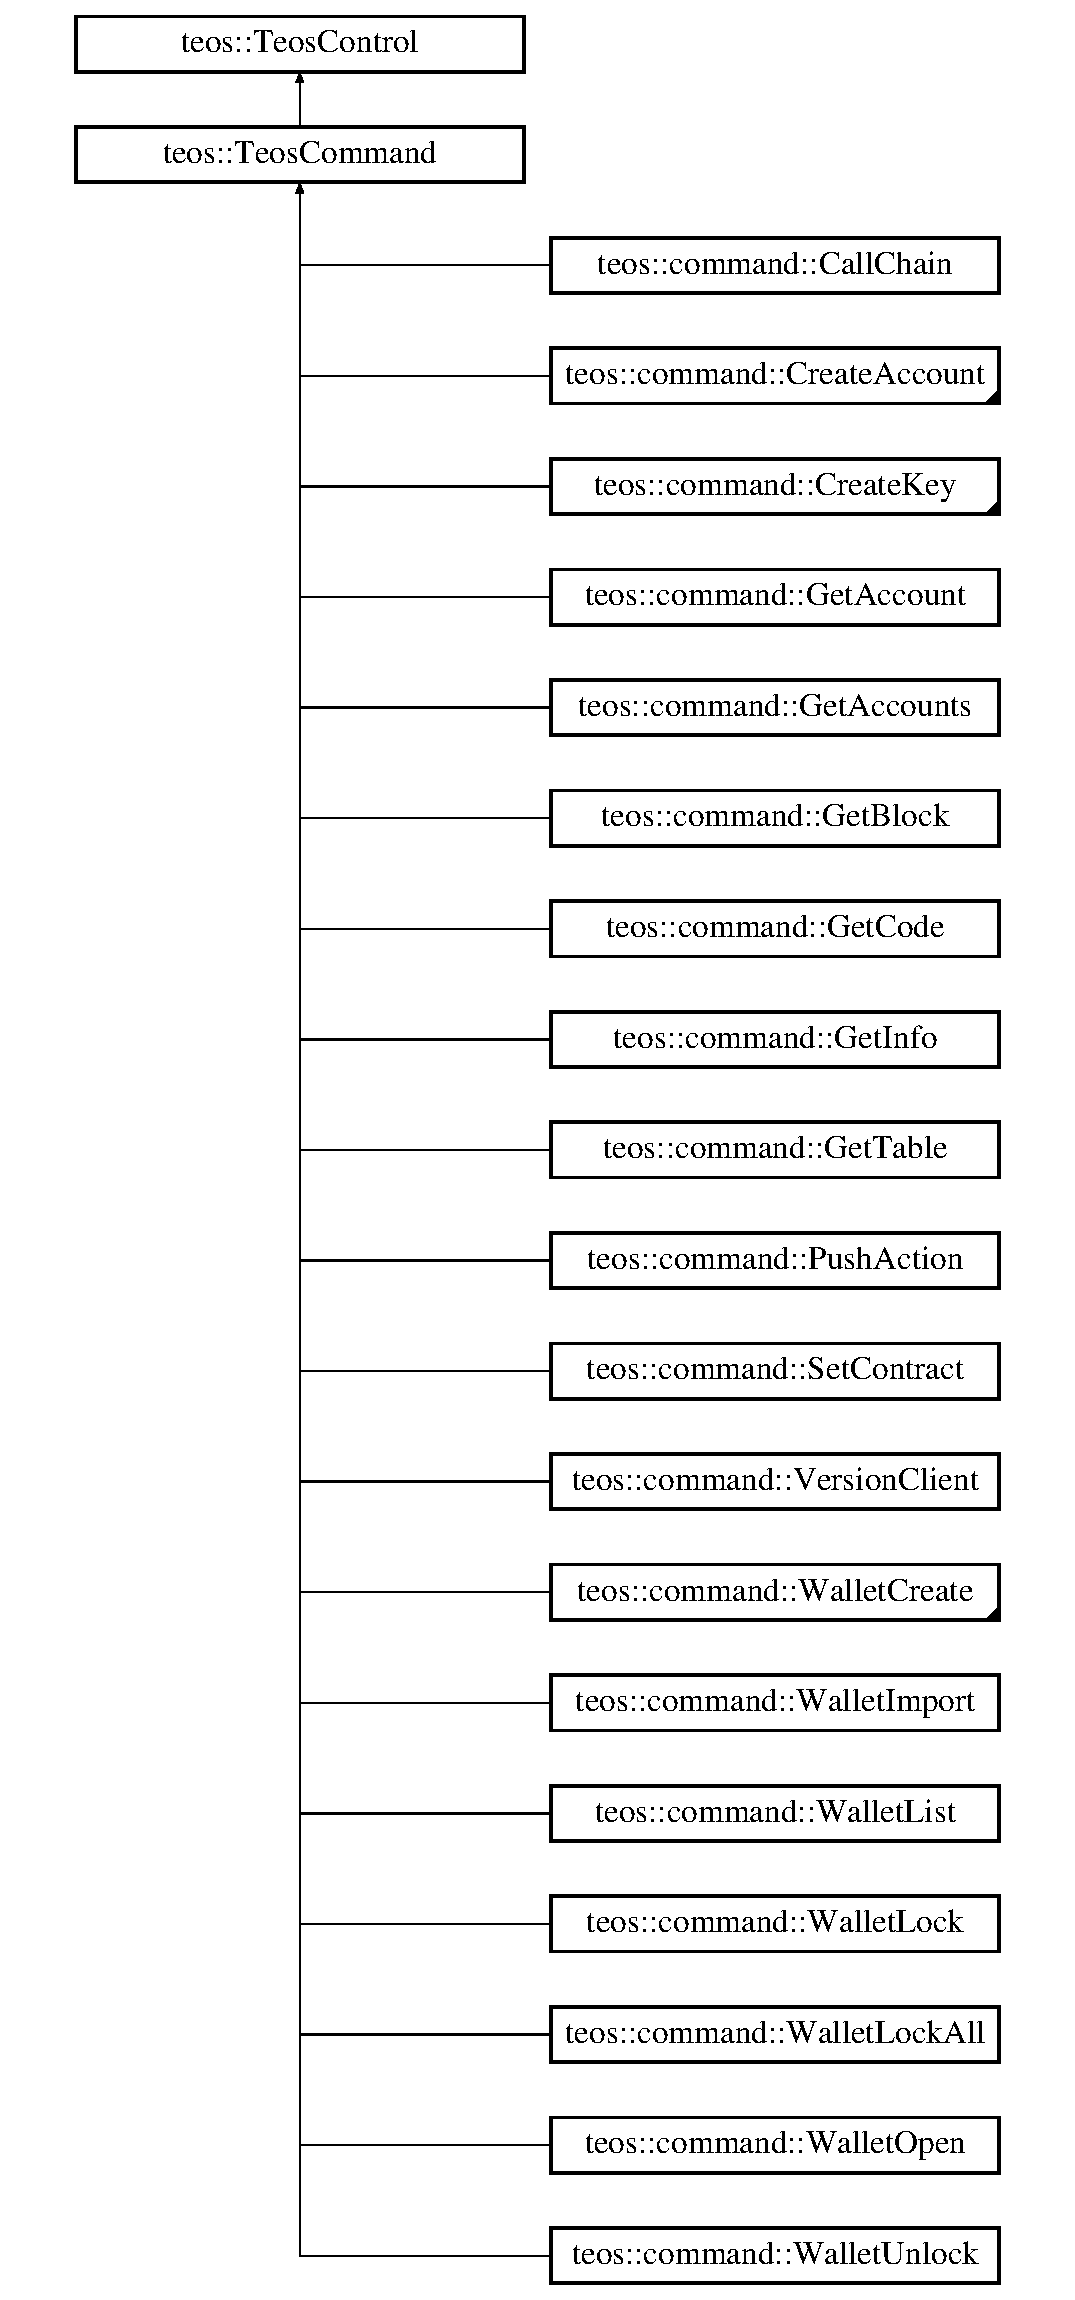
\includegraphics[height=12.000000cm]{classteos_1_1_teos_command}
\end{center}
\end{figure}
\subsection*{Public Member Functions}
\begin{DoxyCompactItemize}
\item 
\mbox{\Hypertarget{classteos_1_1_teos_command_a914843fee0b714f96176109cafee4014}\label{classteos_1_1_teos_command_a914843fee0b714f96176109cafee4014}} 
{\bfseries Teos\+Command} (string path, ptree req\+Json)
\item 
\mbox{\Hypertarget{classteos_1_1_teos_command_a2b68fe1c3c46f20a1e28e6f468c0a8e0}\label{classteos_1_1_teos_command_a2b68fe1c3c46f20a1e28e6f468c0a8e0}} 
{\bfseries Teos\+Command} (string path)
\item 
\mbox{\Hypertarget{classteos_1_1_teos_command_a0d0b0d10829ec7178ba2f9f85db2b67f}\label{classteos_1_1_teos_command_a0d0b0d10829ec7178ba2f9f85db2b67f}} 
{\bfseries Teos\+Command} (string error\+Msg, string error\+Sender)
\item 
\mbox{\Hypertarget{classteos_1_1_teos_command_a3728e4e87c485b4acb46f0d5c88595ad}\label{classteos_1_1_teos_command_a3728e4e87c485b4acb46f0d5c88595ad}} 
void {\bfseries copy} (\mbox{\hyperlink{classteos_1_1_teos_command}{Teos\+Command}} teos\+Command)
\end{DoxyCompactItemize}
\subsection*{Static Public Attributes}
\begin{DoxyCompactItemize}
\item 
\mbox{\Hypertarget{classteos_1_1_teos_command_a54be6ca51cd5c3b55b4fd5506319fcaa}\label{classteos_1_1_teos_command_a54be6ca51cd5c3b55b4fd5506319fcaa}} 
static string {\bfseries http\+Address} = \char`\"{}\char`\"{}
\item 
\mbox{\Hypertarget{classteos_1_1_teos_command_a3c420a38e2e983faab8a32d26c211a0d}\label{classteos_1_1_teos_command_a3c420a38e2e983faab8a32d26c211a0d}} 
static string {\bfseries http\+Wallet\+Address} = \char`\"{}\char`\"{}
\end{DoxyCompactItemize}
\subsection*{Protected Member Functions}
\begin{DoxyCompactItemize}
\item 
\mbox{\Hypertarget{classteos_1_1_teos_command_ac770c5eabcc7bfc6d4a8a8b2b0443458}\label{classteos_1_1_teos_command_ac770c5eabcc7bfc6d4a8a8b2b0443458}} 
void {\bfseries call\+Eosd} ()
\item 
\mbox{\Hypertarget{classteos_1_1_teos_command_abcdc20d75a8e8278cdcae8f0bb482515}\label{classteos_1_1_teos_command_abcdc20d75a8e8278cdcae8f0bb482515}} 
virtual string {\bfseries norm\+Request} (ptree \&req\+Json)
\item 
\mbox{\Hypertarget{classteos_1_1_teos_command_afc2c37d50b3fda078ce3195d9922ab8e}\label{classteos_1_1_teos_command_afc2c37d50b3fda078ce3195d9922ab8e}} 
virtual void {\bfseries norm\+Response} (string response, ptree \&resp\+Json)
\item 
\mbox{\Hypertarget{classteos_1_1_teos_command_a5f377d19a8bb692b2c3008d4b916a950}\label{classteos_1_1_teos_command_a5f377d19a8bb692b2c3008d4b916a950}} 
virtual bool {\bfseries is\+Wallet\+Command} ()
\end{DoxyCompactItemize}
\subsection*{Protected Attributes}
\begin{DoxyCompactItemize}
\item 
\mbox{\Hypertarget{classteos_1_1_teos_command_a263794bdfe8ef1ee2e01e8a5253495f9}\label{classteos_1_1_teos_command_a263794bdfe8ef1ee2e01e8a5253495f9}} 
string {\bfseries path\+\_\+}
\end{DoxyCompactItemize}
\subsection*{Additional Inherited Members}


The documentation for this class was generated from the following files\+:\begin{DoxyCompactItemize}
\item 
include/teoslib/\mbox{\hyperlink{command_8hpp}{command.\+hpp}}\item 
command.\+cpp\end{DoxyCompactItemize}

\hypertarget{classteos_1_1_teos_control}{}\section{teos\+:\+:Teos\+Control Class Reference}
\label{classteos_1_1_teos_control}\index{teos\+::\+Teos\+Control@{teos\+::\+Teos\+Control}}
Inheritance diagram for teos\+:\+:Teos\+Control\+:\begin{figure}[H]
\begin{center}
\leavevmode
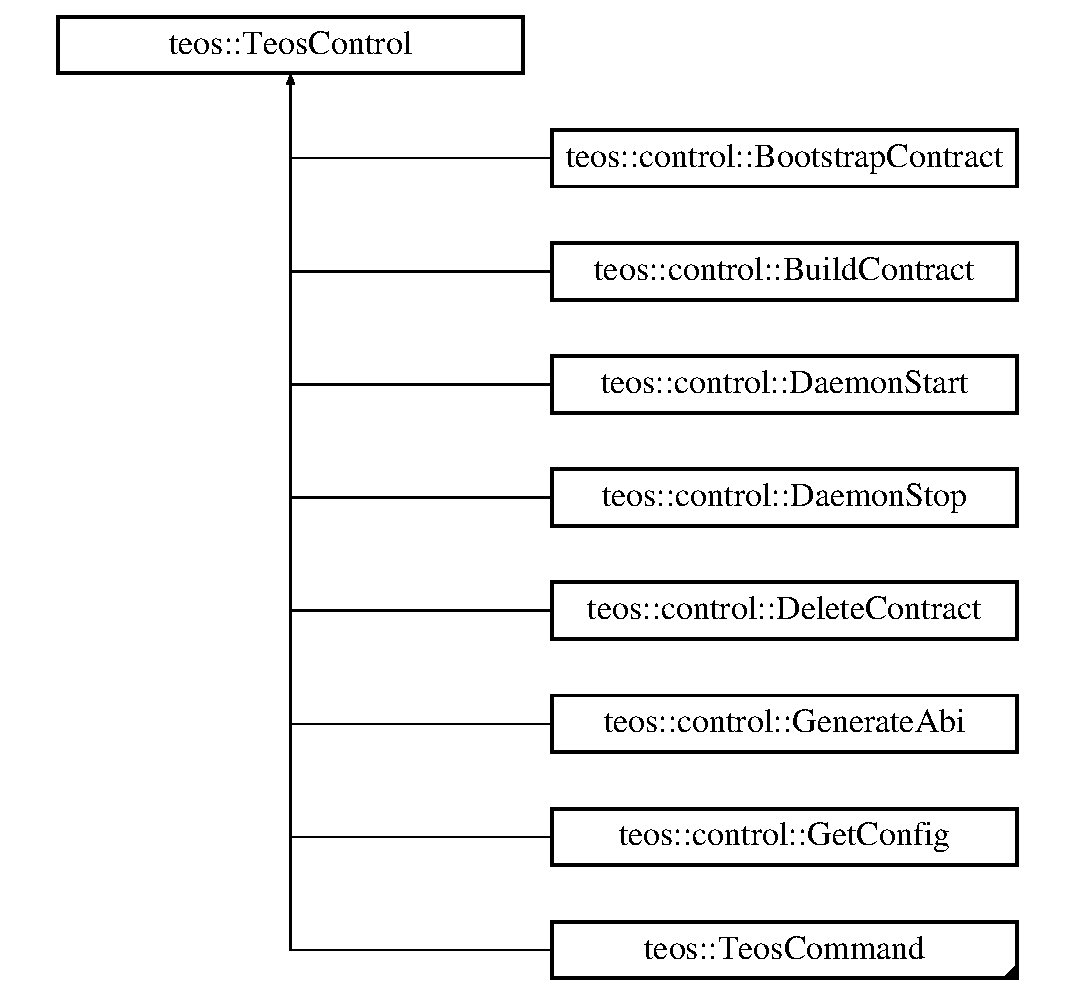
\includegraphics[height=9.000000cm]{classteos_1_1_teos_control}
\end{center}
\end{figure}
\subsection*{Public Member Functions}
\begin{DoxyCompactItemize}
\item 
\mbox{\Hypertarget{classteos_1_1_teos_control_aaa5b0b70263ef6f963636dc43230ef33}\label{classteos_1_1_teos_control_aaa5b0b70263ef6f963636dc43230ef33}} 
void {\bfseries validate\+Json\+Data} (string data, ptree \&json)
\item 
\mbox{\Hypertarget{classteos_1_1_teos_control_abe614f0745845a707ec5c4e0457ebcc0}\label{classteos_1_1_teos_control_abe614f0745845a707ec5c4e0457ebcc0}} 
void {\bfseries error\+Resp\+Json} (string sender, string message)
\item 
\mbox{\Hypertarget{classteos_1_1_teos_control_ad5d500a5c6027ab6c4c9edee0affcf0c}\label{classteos_1_1_teos_control_ad5d500a5c6027ab6c4c9edee0affcf0c}} 
void {\bfseries put\+Error} (string msg, string sender=\char`\"{}\char`\"{})
\item 
\mbox{\Hypertarget{classteos_1_1_teos_control_a005069a333bfa46592633d1bdb1df308}\label{classteos_1_1_teos_control_a005069a333bfa46592633d1bdb1df308}} 
bool {\bfseries print\+Error} ()
\item 
\mbox{\Hypertarget{classteos_1_1_teos_control_a52f86bb515d91acf6cfdccd3fc766187}\label{classteos_1_1_teos_control_a52f86bb515d91acf6cfdccd3fc766187}} 
{\bfseries Teos\+Control} (ptree req\+Json)
\item 
\mbox{\Hypertarget{classteos_1_1_teos_control_af23d4fb6c90c83e47bc6917b3add9da7}\label{classteos_1_1_teos_control_af23d4fb6c90c83e47bc6917b3add9da7}} 
string {\bfseries error\+Msg} ()
\item 
\mbox{\Hypertarget{classteos_1_1_teos_control_af14d89eea741cfc345db34bd2ba75d0b}\label{classteos_1_1_teos_control_af14d89eea741cfc345db34bd2ba75d0b}} 
string {\bfseries request\+To\+String} (bool is\+Raw=false) const
\item 
\mbox{\Hypertarget{classteos_1_1_teos_control_a5a4f418dfe30ab50fb373e341b9974db}\label{classteos_1_1_teos_control_a5a4f418dfe30ab50fb373e341b9974db}} 
string {\bfseries response\+To\+String} (bool is\+Raw=false) const
\item 
\mbox{\Hypertarget{classteos_1_1_teos_control_ae5781470510c9bb90a3ef0917e72b1b8}\label{classteos_1_1_teos_control_ae5781470510c9bb90a3ef0917e72b1b8}} 
{\footnotesize template$<$typename Type $>$ }\\Type {\bfseries get} (const ptree\+::path\+\_\+type \&path) const
\item 
\mbox{\Hypertarget{classteos_1_1_teos_control_aa318124d7a906e4b1391fae5ad50cfb0}\label{classteos_1_1_teos_control_aa318124d7a906e4b1391fae5ad50cfb0}} 
void {\bfseries copy} (\mbox{\hyperlink{classteos_1_1_teos_control}{Teos\+Control}} teos\+Command)
\end{DoxyCompactItemize}
\subsection*{Public Attributes}
\begin{DoxyCompactItemize}
\item 
\mbox{\Hypertarget{classteos_1_1_teos_control_ac8e6788b523dcd724c7a424818da7849}\label{classteos_1_1_teos_control_ac8e6788b523dcd724c7a424818da7849}} 
bool {\bfseries is\+Error\+\_\+}
\item 
\mbox{\Hypertarget{classteos_1_1_teos_control_a6122f1a2263a80dacd315739861feac7}\label{classteos_1_1_teos_control_a6122f1a2263a80dacd315739861feac7}} 
ptree {\bfseries req\+Json\+\_\+}
\item 
\mbox{\Hypertarget{classteos_1_1_teos_control_a1f5268be242e9f6182a083a4d4ec393e}\label{classteos_1_1_teos_control_a1f5268be242e9f6182a083a4d4ec393e}} 
ptree {\bfseries resp\+Json\+\_\+}
\end{DoxyCompactItemize}


The documentation for this class was generated from the following files\+:\begin{DoxyCompactItemize}
\item 
teos\+\_\+lib/include/teoslib/control.\+hpp\item 
teos\+\_\+lib/control.\+cpp\end{DoxyCompactItemize}

\hypertarget{classteos_1_1command_1_1_version_client}{}\section{teos\+:\+:command\+:\+:Version\+Client Class Reference}
\label{classteos_1_1command_1_1_version_client}\index{teos\+::command\+::\+Version\+Client@{teos\+::command\+::\+Version\+Client}}
Inheritance diagram for teos\+:\+:command\+:\+:Version\+Client\+:\begin{figure}[H]
\begin{center}
\leavevmode
\includegraphics[height=3.000000cm]{classteos_1_1command_1_1_version_client}
\end{center}
\end{figure}
\subsection*{Public Member Functions}
\begin{DoxyCompactItemize}
\item 
\mbox{\Hypertarget{classteos_1_1command_1_1_version_client_a90072a3531e0e9064ff5933fea90807e}\label{classteos_1_1command_1_1_version_client_a90072a3531e0e9064ff5933fea90807e}} 
{\bfseries Version\+Client} (ptree req\+Json)
\end{DoxyCompactItemize}
\subsection*{Additional Inherited Members}


The documentation for this class was generated from the following file\+:\begin{DoxyCompactItemize}
\item 
teos\+\_\+lib/include/teoslib/command/other\+\_\+commands.\+hpp\end{DoxyCompactItemize}

\hypertarget{classteos_1_1command_1_1_version_client_options}{}\section{teos\+:\+:command\+:\+:Version\+Client\+Options Class Reference}
\label{classteos_1_1command_1_1_version_client_options}\index{teos\+::command\+::\+Version\+Client\+Options@{teos\+::command\+::\+Version\+Client\+Options}}
Inheritance diagram for teos\+:\+:command\+:\+:Version\+Client\+Options\+:\begin{figure}[H]
\begin{center}
\leavevmode
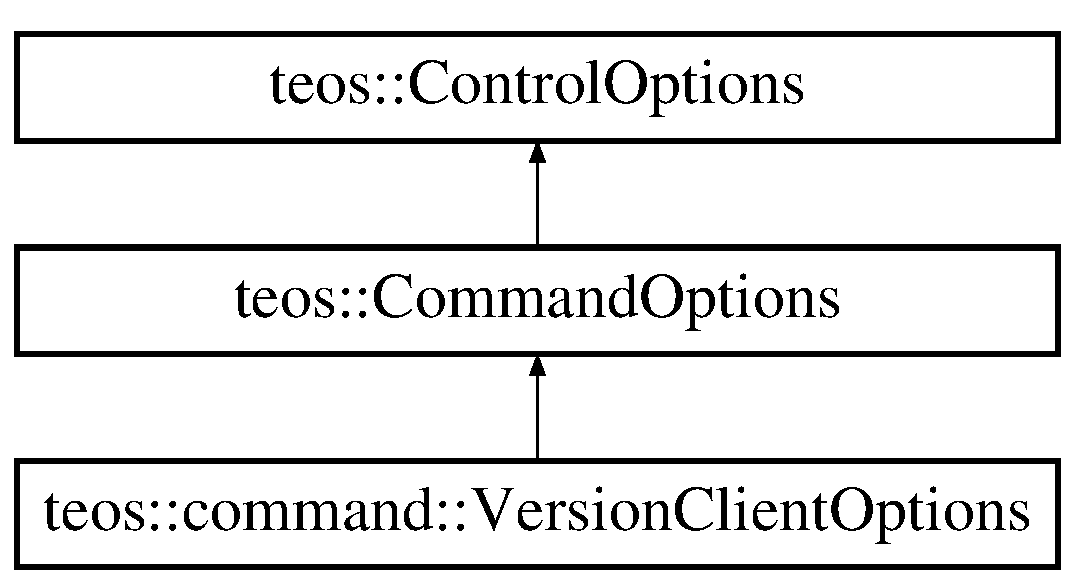
\includegraphics[height=3.000000cm]{classteos_1_1command_1_1_version_client_options}
\end{center}
\end{figure}
\subsection*{Public Member Functions}
\begin{DoxyCompactItemize}
\item 
\mbox{\Hypertarget{classteos_1_1command_1_1_version_client_options_a989412affdf0f88746ddb855434412e6}\label{classteos_1_1command_1_1_version_client_options_a989412affdf0f88746ddb855434412e6}} 
{\bfseries Version\+Client\+Options} (int argc, const char $\ast$$\ast$argv)
\end{DoxyCompactItemize}
\subsection*{Protected Member Functions}
\begin{DoxyCompactItemize}
\item 
const char $\ast$ \mbox{\hyperlink{classteos_1_1command_1_1_version_client_options_a28b69107e8eb50a2faf9594958bb1d6d}{get\+Usage}} ()
\begin{DoxyCompactList}\small\item\em Command \textquotesingle{}usage\textquotesingle{} instruction. \end{DoxyCompactList}\item 
\mbox{\Hypertarget{classteos_1_1command_1_1_version_client_options_a8cd89cab3d5a38971de1c75facc7a47d}\label{classteos_1_1command_1_1_version_client_options_a8cd89cab3d5a38971de1c75facc7a47d}} 
\mbox{\hyperlink{classteos_1_1_teos_control}{Teos\+Control}} {\bfseries execute\+Command} ()
\item 
\mbox{\Hypertarget{classteos_1_1command_1_1_version_client_options_a1b6021ecadaaed16af399487d573b9f1}\label{classteos_1_1command_1_1_version_client_options_a1b6021ecadaaed16af399487d573b9f1}} 
void {\bfseries printout} (\mbox{\hyperlink{classteos_1_1_teos_control}{Teos\+Control}} command, variables\+\_\+map \&vm)
\end{DoxyCompactItemize}
\subsection*{Additional Inherited Members}


\subsection{Member Function Documentation}
\mbox{\Hypertarget{classteos_1_1command_1_1_version_client_options_a28b69107e8eb50a2faf9594958bb1d6d}\label{classteos_1_1command_1_1_version_client_options_a28b69107e8eb50a2faf9594958bb1d6d}} 
\index{teos\+::command\+::\+Version\+Client\+Options@{teos\+::command\+::\+Version\+Client\+Options}!get\+Usage@{get\+Usage}}
\index{get\+Usage@{get\+Usage}!teos\+::command\+::\+Version\+Client\+Options@{teos\+::command\+::\+Version\+Client\+Options}}
\subsubsection{\texorpdfstring{get\+Usage()}{getUsage()}}
{\footnotesize\ttfamily const char$\ast$ teos\+::command\+::\+Version\+Client\+Options\+::get\+Usage (\begin{DoxyParamCaption}{ }\end{DoxyParamCaption})\hspace{0.3cm}{\ttfamily [inline]}, {\ttfamily [protected]}, {\ttfamily [virtual]}}



Command \textquotesingle{}usage\textquotesingle{} instruction. 

\begin{DoxyReturn}{Returns}
usage text 
\end{DoxyReturn}


Reimplemented from \mbox{\hyperlink{classteos_1_1_control_options_a0aa5671f9bc750ed5280c26c543874f3}{teos\+::\+Control\+Options}}.



The documentation for this class was generated from the following file\+:\begin{DoxyCompactItemize}
\item 
include/teoslib/command/other\+\_\+commands.\+hpp\end{DoxyCompactItemize}

\hypertarget{classteos_1_1command_1_1_wallet_create}{}\section{teos\+:\+:command\+:\+:Wallet\+Create Class Reference}
\label{classteos_1_1command_1_1_wallet_create}\index{teos\+::command\+::\+Wallet\+Create@{teos\+::command\+::\+Wallet\+Create}}


Create a new wallet locall.  




{\ttfamily \#include $<$wallet\+\_\+commands.\+hpp$>$}

Inheritance diagram for teos\+:\+:command\+:\+:Wallet\+Create\+:\begin{figure}[H]
\begin{center}
\leavevmode
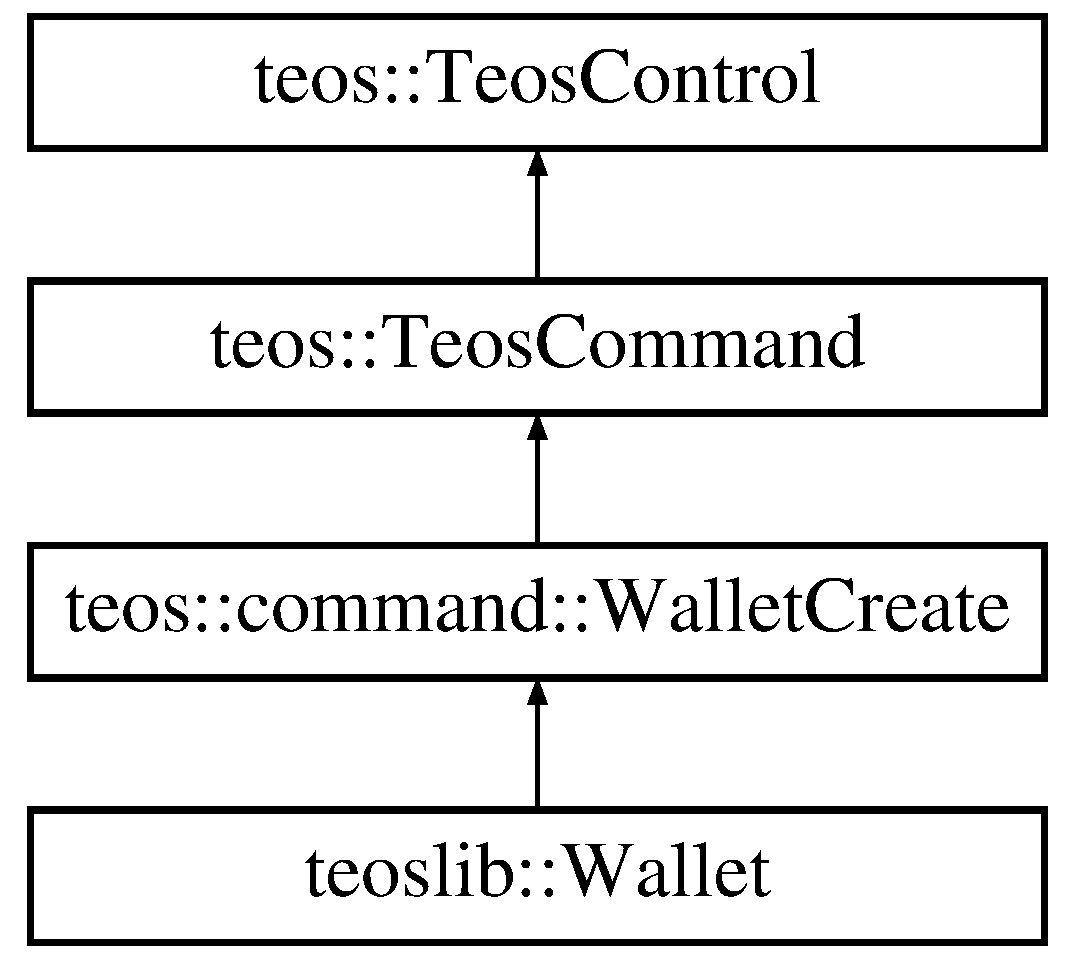
\includegraphics[height=4.000000cm]{classteos_1_1command_1_1_wallet_create}
\end{center}
\end{figure}
\subsection*{Public Member Functions}
\begin{DoxyCompactItemize}
\item 
\mbox{\hyperlink{classteos_1_1command_1_1_wallet_create_a78153f8e5eb577cdeb3734c7229df923}{Wallet\+Create}} (string name=D\+E\+F\+A\+U\+L\+T\+\_\+\+W\+A\+L\+L\+E\+T\+\_\+\+N\+A\+ME)
\begin{DoxyCompactList}\small\item\em A constructor. \end{DoxyCompactList}\item 
\mbox{\hyperlink{classteos_1_1command_1_1_wallet_create_a3a7979db66f2ea69186888d50dd6ce69}{Wallet\+Create}} (ptree req\+Json)
\begin{DoxyCompactList}\small\item\em A constructor. \end{DoxyCompactList}\item 
\mbox{\Hypertarget{classteos_1_1command_1_1_wallet_create_aa95ee68f9139186395722e2028ec6309}\label{classteos_1_1command_1_1_wallet_create_aa95ee68f9139186395722e2028ec6309}} 
string {\bfseries norm\+Request} (ptree \&req\+Json)
\item 
\mbox{\Hypertarget{classteos_1_1command_1_1_wallet_create_a419455a10d7be5d8264dbfe2bfdf511c}\label{classteos_1_1command_1_1_wallet_create_a419455a10d7be5d8264dbfe2bfdf511c}} 
void {\bfseries norm\+Response} (string response, ptree \&resp\+Json)
\end{DoxyCompactItemize}
\subsection*{Additional Inherited Members}


\subsection{Detailed Description}
Create a new wallet locall. 

\subsection{Constructor \& Destructor Documentation}
\mbox{\Hypertarget{classteos_1_1command_1_1_wallet_create_a78153f8e5eb577cdeb3734c7229df923}\label{classteos_1_1command_1_1_wallet_create_a78153f8e5eb577cdeb3734c7229df923}} 
\index{teos\+::command\+::\+Wallet\+Create@{teos\+::command\+::\+Wallet\+Create}!Wallet\+Create@{Wallet\+Create}}
\index{Wallet\+Create@{Wallet\+Create}!teos\+::command\+::\+Wallet\+Create@{teos\+::command\+::\+Wallet\+Create}}
\subsubsection{\texorpdfstring{Wallet\+Create()}{WalletCreate()}\hspace{0.1cm}{\footnotesize\ttfamily [1/2]}}
{\footnotesize\ttfamily teos\+::command\+::\+Wallet\+Create\+::\+Wallet\+Create (\begin{DoxyParamCaption}\item[{string}]{name = {\ttfamily DEFAULT\+\_\+WALLET\+\_\+NAME} }\end{DoxyParamCaption})\hspace{0.3cm}{\ttfamily [inline]}}



A constructor. 


\begin{DoxyParams}{Parameters}
{\em name} & wallet ID. \\
\hline
\end{DoxyParams}
\mbox{\Hypertarget{classteos_1_1command_1_1_wallet_create_a3a7979db66f2ea69186888d50dd6ce69}\label{classteos_1_1command_1_1_wallet_create_a3a7979db66f2ea69186888d50dd6ce69}} 
\index{teos\+::command\+::\+Wallet\+Create@{teos\+::command\+::\+Wallet\+Create}!Wallet\+Create@{Wallet\+Create}}
\index{Wallet\+Create@{Wallet\+Create}!teos\+::command\+::\+Wallet\+Create@{teos\+::command\+::\+Wallet\+Create}}
\subsubsection{\texorpdfstring{Wallet\+Create()}{WalletCreate()}\hspace{0.1cm}{\footnotesize\ttfamily [2/2]}}
{\footnotesize\ttfamily teos\+::command\+::\+Wallet\+Create\+::\+Wallet\+Create (\begin{DoxyParamCaption}\item[{ptree}]{req\+Json }\end{DoxyParamCaption})\hspace{0.3cm}{\ttfamily [inline]}}



A constructor. 


\begin{DoxyParams}{Parameters}
{\em req\+Json} & json tree argument\+: \{\char`\"{}name\char`\"{}\+:\char`\"{}$<$wallet name$>$\char`\"{}\}. \\
\hline
\end{DoxyParams}


The documentation for this class was generated from the following file\+:\begin{DoxyCompactItemize}
\item 
teos\+\_\+lib/include/teoslib/command/wallet\+\_\+commands.\+hpp\end{DoxyCompactItemize}

\hypertarget{classteos_1_1command_1_1_wallet_create_options}{}\section{teos\+:\+:command\+:\+:Wallet\+Create\+Options Class Reference}
\label{classteos_1_1command_1_1_wallet_create_options}\index{teos\+::command\+::\+Wallet\+Create\+Options@{teos\+::command\+::\+Wallet\+Create\+Options}}


Command-\/line driver for the \mbox{\hyperlink{classteos_1_1command_1_1_wallet_create}{Wallet\+Create}} class.  




{\ttfamily \#include $<$wallet\+\_\+commands.\+hpp$>$}

Inheritance diagram for teos\+:\+:command\+:\+:Wallet\+Create\+Options\+:\begin{figure}[H]
\begin{center}
\leavevmode
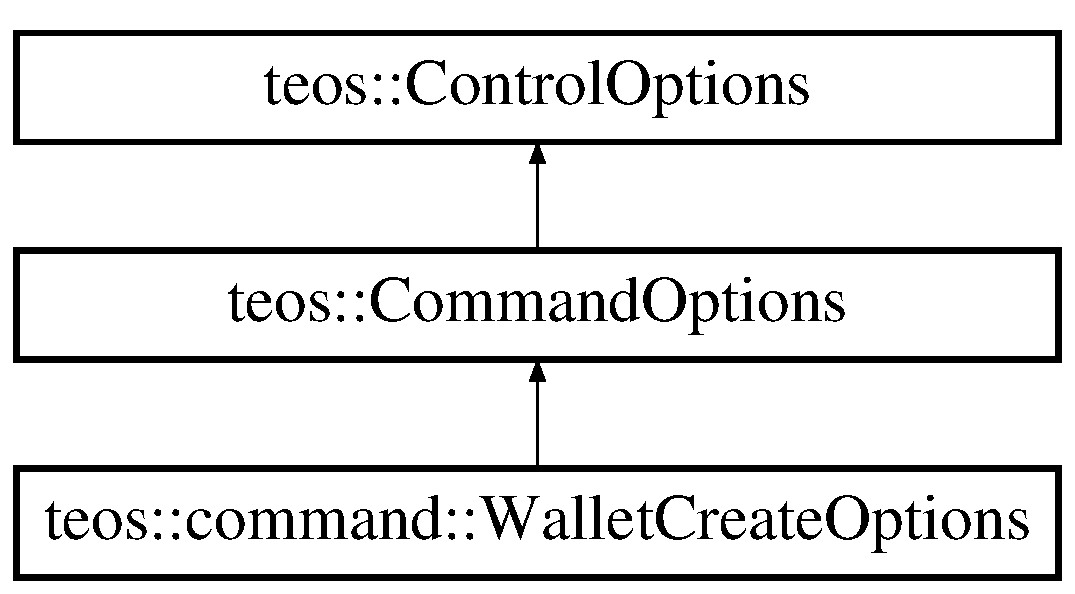
\includegraphics[height=3.000000cm]{classteos_1_1command_1_1_wallet_create_options}
\end{center}
\end{figure}
\subsection*{Public Member Functions}
\begin{DoxyCompactItemize}
\item 
\mbox{\Hypertarget{classteos_1_1command_1_1_wallet_create_options_adfecccb1465e96428f2bac21dc4202f6}\label{classteos_1_1command_1_1_wallet_create_options_adfecccb1465e96428f2bac21dc4202f6}} 
{\bfseries Wallet\+Create\+Options} (int argc, const char $\ast$$\ast$argv)
\end{DoxyCompactItemize}
\subsection*{Protected Member Functions}
\begin{DoxyCompactItemize}
\item 
const char $\ast$ \mbox{\hyperlink{classteos_1_1command_1_1_wallet_create_options_ad20c1955cb48f6c9e640c35eae091c30}{get\+Usage}} ()
\begin{DoxyCompactList}\small\item\em Command \textquotesingle{}usage\textquotesingle{} instruction. \end{DoxyCompactList}\item 
\mbox{\Hypertarget{classteos_1_1command_1_1_wallet_create_options_a03ae823b5d36d609fef32fee4bc8e91b}\label{classteos_1_1command_1_1_wallet_create_options_a03ae823b5d36d609fef32fee4bc8e91b}} 
options\+\_\+description {\bfseries argument\+Description} ()
\item 
\mbox{\Hypertarget{classteos_1_1command_1_1_wallet_create_options_aa7b5f9da2a345df6998a329f6e07e021}\label{classteos_1_1command_1_1_wallet_create_options_aa7b5f9da2a345df6998a329f6e07e021}} 
void {\bfseries set\+Pos\+Desc} (positional\+\_\+options\+\_\+description \&pos\+\_\+desc)
\item 
\mbox{\Hypertarget{classteos_1_1command_1_1_wallet_create_options_a48cc1abd55a90c1b04c3cd69922efaec}\label{classteos_1_1command_1_1_wallet_create_options_a48cc1abd55a90c1b04c3cd69922efaec}} 
bool {\bfseries check\+Arguments} (variables\+\_\+map \&vm)
\item 
\mbox{\Hypertarget{classteos_1_1command_1_1_wallet_create_options_a4865f7273086dd8cda1234ff72862bab}\label{classteos_1_1command_1_1_wallet_create_options_a4865f7273086dd8cda1234ff72862bab}} 
\mbox{\hyperlink{classteos_1_1_teos_control}{Teos\+Control}} {\bfseries execute\+Command} ()
\item 
\mbox{\Hypertarget{classteos_1_1command_1_1_wallet_create_options_a78875cc06e1509c794a265f2b1805259}\label{classteos_1_1command_1_1_wallet_create_options_a78875cc06e1509c794a265f2b1805259}} 
void {\bfseries printout} (\mbox{\hyperlink{classteos_1_1_teos_control}{Teos\+Control}} command, variables\+\_\+map \&vm)
\end{DoxyCompactItemize}
\subsection*{Protected Attributes}
\begin{DoxyCompactItemize}
\item 
\mbox{\Hypertarget{classteos_1_1command_1_1_wallet_create_options_a0a3fb5e1bc5be7c997b829ecfec7ad6b}\label{classteos_1_1command_1_1_wallet_create_options_a0a3fb5e1bc5be7c997b829ecfec7ad6b}} 
string {\bfseries name}
\end{DoxyCompactItemize}
\subsection*{Additional Inherited Members}


\subsection{Detailed Description}
Command-\/line driver for the \mbox{\hyperlink{classteos_1_1command_1_1_wallet_create}{Wallet\+Create}} class. 

\subsection{Member Function Documentation}
\mbox{\Hypertarget{classteos_1_1command_1_1_wallet_create_options_ad20c1955cb48f6c9e640c35eae091c30}\label{classteos_1_1command_1_1_wallet_create_options_ad20c1955cb48f6c9e640c35eae091c30}} 
\index{teos\+::command\+::\+Wallet\+Create\+Options@{teos\+::command\+::\+Wallet\+Create\+Options}!get\+Usage@{get\+Usage}}
\index{get\+Usage@{get\+Usage}!teos\+::command\+::\+Wallet\+Create\+Options@{teos\+::command\+::\+Wallet\+Create\+Options}}
\subsubsection{\texorpdfstring{get\+Usage()}{getUsage()}}
{\footnotesize\ttfamily const char$\ast$ teos\+::command\+::\+Wallet\+Create\+Options\+::get\+Usage (\begin{DoxyParamCaption}{ }\end{DoxyParamCaption})\hspace{0.3cm}{\ttfamily [inline]}, {\ttfamily [protected]}, {\ttfamily [virtual]}}



Command \textquotesingle{}usage\textquotesingle{} instruction. 

\begin{DoxyReturn}{Returns}
usage text 
\end{DoxyReturn}


Reimplemented from \mbox{\hyperlink{classteos_1_1_control_options_a0aa5671f9bc750ed5280c26c543874f3}{teos\+::\+Control\+Options}}.



The documentation for this class was generated from the following file\+:\begin{DoxyCompactItemize}
\item 
include/teoslib/command/wallet\+\_\+commands.\+hpp\end{DoxyCompactItemize}

\hypertarget{classteos_1_1command_1_1_wallet_import}{}\section{teos\+:\+:command\+:\+:Wallet\+Import Class Reference}
\label{classteos_1_1command_1_1_wallet_import}\index{teos\+::command\+::\+Wallet\+Import@{teos\+::command\+::\+Wallet\+Import}}


Import private key into wallet.  




{\ttfamily \#include $<$wallet\+\_\+commands.\+hpp$>$}

Inheritance diagram for teos\+:\+:command\+:\+:Wallet\+Import\+:\begin{figure}[H]
\begin{center}
\leavevmode
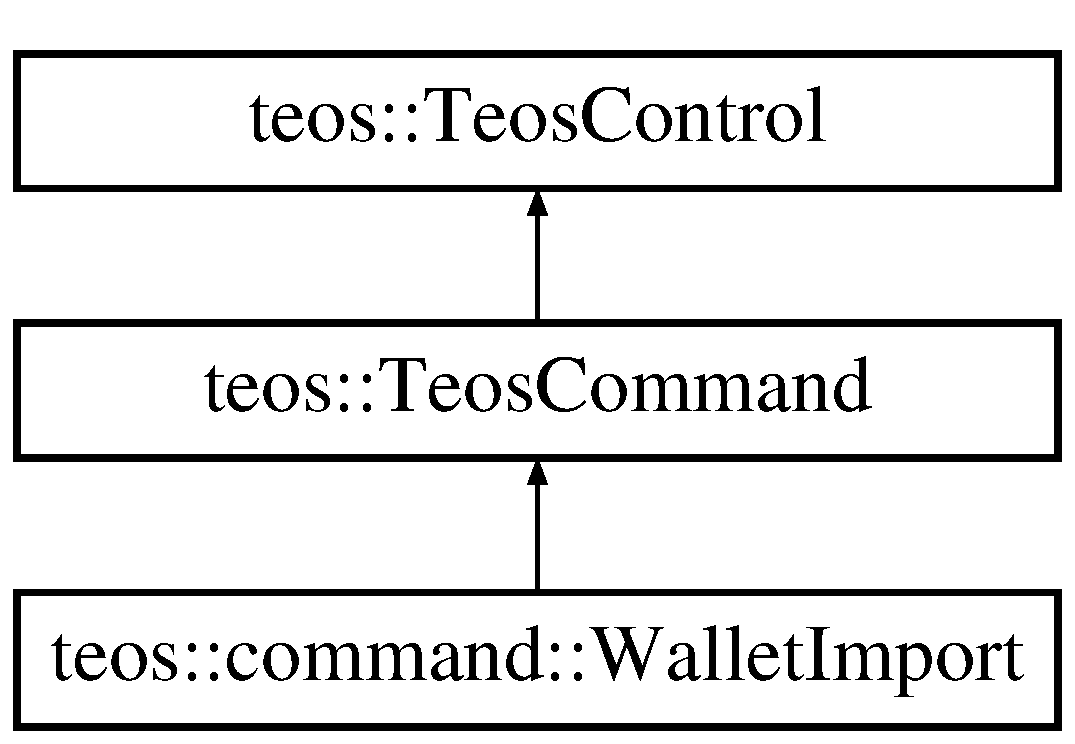
\includegraphics[height=3.000000cm]{classteos_1_1command_1_1_wallet_import}
\end{center}
\end{figure}
\subsection*{Public Member Functions}
\begin{DoxyCompactItemize}
\item 
\mbox{\hyperlink{classteos_1_1command_1_1_wallet_import_afcf1166b4ac17b4cd6cfeb02cbba7233}{Wallet\+Import}} (string name, string key\+Private)
\begin{DoxyCompactList}\small\item\em A constructor. \end{DoxyCompactList}\item 
\mbox{\hyperlink{classteos_1_1command_1_1_wallet_import_af8b0bf00655b26891fa3091aa4e92907}{Wallet\+Import}} (ptree req\+Json)
\begin{DoxyCompactList}\small\item\em A constructor. \end{DoxyCompactList}\item 
\mbox{\Hypertarget{classteos_1_1command_1_1_wallet_import_a9f2be518b7a2fdd12573a93bc29c92a7}\label{classteos_1_1command_1_1_wallet_import_a9f2be518b7a2fdd12573a93bc29c92a7}} 
string {\bfseries norm\+Request} (ptree \&req\+Json)
\item 
\mbox{\Hypertarget{classteos_1_1command_1_1_wallet_import_ae4a1ce8284a4482555c778f2aca17722}\label{classteos_1_1command_1_1_wallet_import_ae4a1ce8284a4482555c778f2aca17722}} 
void {\bfseries norm\+Response} (string response, ptree \&resp\+Json)
\end{DoxyCompactItemize}
\subsection*{Additional Inherited Members}


\subsection{Detailed Description}
Import private key into wallet. 

\subsection{Constructor \& Destructor Documentation}
\mbox{\Hypertarget{classteos_1_1command_1_1_wallet_import_afcf1166b4ac17b4cd6cfeb02cbba7233}\label{classteos_1_1command_1_1_wallet_import_afcf1166b4ac17b4cd6cfeb02cbba7233}} 
\index{teos\+::command\+::\+Wallet\+Import@{teos\+::command\+::\+Wallet\+Import}!Wallet\+Import@{Wallet\+Import}}
\index{Wallet\+Import@{Wallet\+Import}!teos\+::command\+::\+Wallet\+Import@{teos\+::command\+::\+Wallet\+Import}}
\subsubsection{\texorpdfstring{Wallet\+Import()}{WalletImport()}\hspace{0.1cm}{\footnotesize\ttfamily [1/2]}}
{\footnotesize\ttfamily teos\+::command\+::\+Wallet\+Import\+::\+Wallet\+Import (\begin{DoxyParamCaption}\item[{string}]{name,  }\item[{string}]{key\+Private }\end{DoxyParamCaption})\hspace{0.3cm}{\ttfamily [inline]}}



A constructor. 


\begin{DoxyParams}{Parameters}
{\em name} & wallet ID. \\
\hline
{\em key\+Private} & private key, proving authorities. \\
\hline
\end{DoxyParams}
\mbox{\Hypertarget{classteos_1_1command_1_1_wallet_import_af8b0bf00655b26891fa3091aa4e92907}\label{classteos_1_1command_1_1_wallet_import_af8b0bf00655b26891fa3091aa4e92907}} 
\index{teos\+::command\+::\+Wallet\+Import@{teos\+::command\+::\+Wallet\+Import}!Wallet\+Import@{Wallet\+Import}}
\index{Wallet\+Import@{Wallet\+Import}!teos\+::command\+::\+Wallet\+Import@{teos\+::command\+::\+Wallet\+Import}}
\subsubsection{\texorpdfstring{Wallet\+Import()}{WalletImport()}\hspace{0.1cm}{\footnotesize\ttfamily [2/2]}}
{\footnotesize\ttfamily teos\+::command\+::\+Wallet\+Import\+::\+Wallet\+Import (\begin{DoxyParamCaption}\item[{ptree}]{req\+Json }\end{DoxyParamCaption})\hspace{0.3cm}{\ttfamily [inline]}}



A constructor. 


\begin{DoxyParams}{Parameters}
{\em req\+Json} & json tree argument\+: \{\char`\"{}name\char`\"{}\+:\char`\"{}$<$wallet name$>$\char`\"{}, \char`\"{}key\char`\"{}\+:\char`\"{}$<$private key$>$\char`\"{}\}. \\
\hline
\end{DoxyParams}


The documentation for this class was generated from the following file\+:\begin{DoxyCompactItemize}
\item 
teos\+\_\+lib/include/teoslib/command/wallet\+\_\+commands.\+hpp\end{DoxyCompactItemize}

\hypertarget{classteos_1_1command_1_1_wallet_import_options}{}\section{teos\+:\+:command\+:\+:Wallet\+Import\+Options Class Reference}
\label{classteos_1_1command_1_1_wallet_import_options}\index{teos\+::command\+::\+Wallet\+Import\+Options@{teos\+::command\+::\+Wallet\+Import\+Options}}


Command-\/line driver for the \mbox{\hyperlink{classteos_1_1command_1_1_wallet_import}{Wallet\+Import}} class.  




{\ttfamily \#include $<$wallet\+\_\+commands.\+hpp$>$}

Inheritance diagram for teos\+:\+:command\+:\+:Wallet\+Import\+Options\+:\begin{figure}[H]
\begin{center}
\leavevmode
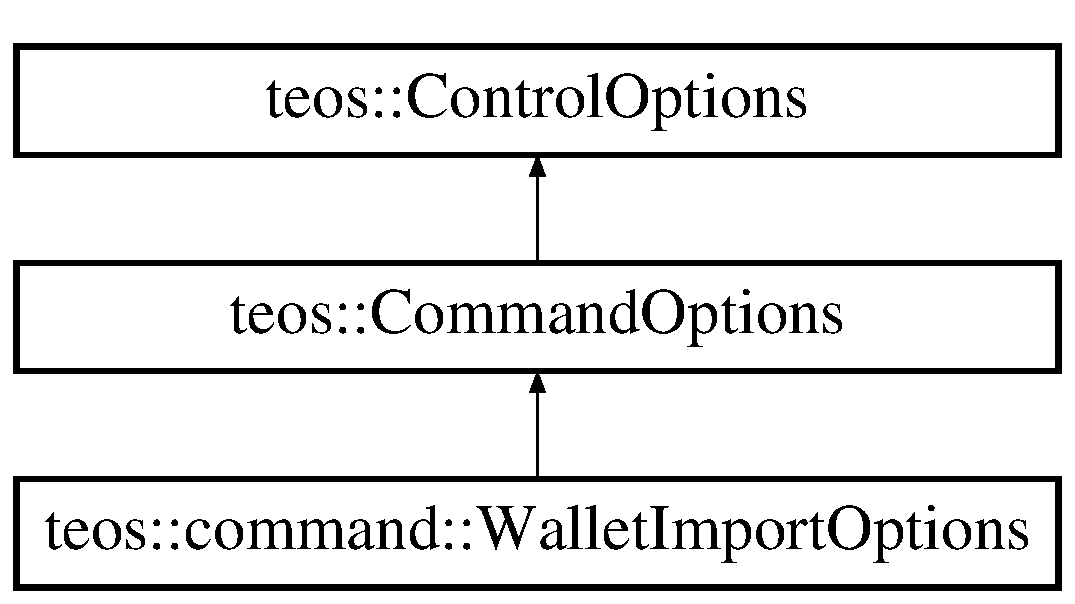
\includegraphics[height=3.000000cm]{classteos_1_1command_1_1_wallet_import_options}
\end{center}
\end{figure}
\subsection*{Public Member Functions}
\begin{DoxyCompactItemize}
\item 
\mbox{\Hypertarget{classteos_1_1command_1_1_wallet_import_options_a7149c93315a38b07515b96640f810ad0}\label{classteos_1_1command_1_1_wallet_import_options_a7149c93315a38b07515b96640f810ad0}} 
{\bfseries Wallet\+Import\+Options} (int argc, const char $\ast$$\ast$argv)
\end{DoxyCompactItemize}
\subsection*{Protected Member Functions}
\begin{DoxyCompactItemize}
\item 
const char $\ast$ \mbox{\hyperlink{classteos_1_1command_1_1_wallet_import_options_ad641b37bd61f2d4ff3e3049e2dd6be0e}{get\+Usage}} ()
\begin{DoxyCompactList}\small\item\em Command \textquotesingle{}usage\textquotesingle{} instruction. \end{DoxyCompactList}\item 
\mbox{\Hypertarget{classteos_1_1command_1_1_wallet_import_options_a5b23093e1d0189769adcbd8f9bbd8d3a}\label{classteos_1_1command_1_1_wallet_import_options_a5b23093e1d0189769adcbd8f9bbd8d3a}} 
options\+\_\+description {\bfseries argument\+Description} ()
\item 
\mbox{\Hypertarget{classteos_1_1command_1_1_wallet_import_options_a33c430a28ea488b0736bb9a09a7f3908}\label{classteos_1_1command_1_1_wallet_import_options_a33c430a28ea488b0736bb9a09a7f3908}} 
void {\bfseries set\+Pos\+Desc} (positional\+\_\+options\+\_\+description \&pos\+\_\+desc)
\item 
\mbox{\Hypertarget{classteos_1_1command_1_1_wallet_import_options_a0b788a2c585f9c9df79c4be401bd8ebb}\label{classteos_1_1command_1_1_wallet_import_options_a0b788a2c585f9c9df79c4be401bd8ebb}} 
bool {\bfseries check\+Arguments} (variables\+\_\+map \&vm)
\item 
\mbox{\Hypertarget{classteos_1_1command_1_1_wallet_import_options_ac0ecd44469164674a49462711d213532}\label{classteos_1_1command_1_1_wallet_import_options_ac0ecd44469164674a49462711d213532}} 
\mbox{\hyperlink{classteos_1_1_teos_control}{Teos\+Control}} {\bfseries execute\+Command} ()
\item 
\mbox{\Hypertarget{classteos_1_1command_1_1_wallet_import_options_a45ecbc443e738c6da3e8d7416cfa4468}\label{classteos_1_1command_1_1_wallet_import_options_a45ecbc443e738c6da3e8d7416cfa4468}} 
void {\bfseries printout} (\mbox{\hyperlink{classteos_1_1_teos_control}{Teos\+Control}} command, variables\+\_\+map \&vm)
\end{DoxyCompactItemize}
\subsection*{Protected Attributes}
\begin{DoxyCompactItemize}
\item 
\mbox{\Hypertarget{classteos_1_1command_1_1_wallet_import_options_af3d4f31c9434cbae7325ac094cbefa30}\label{classteos_1_1command_1_1_wallet_import_options_af3d4f31c9434cbae7325ac094cbefa30}} 
string {\bfseries name}
\item 
\mbox{\Hypertarget{classteos_1_1command_1_1_wallet_import_options_af81e0809fede96b8d0b627d141e80cc3}\label{classteos_1_1command_1_1_wallet_import_options_af81e0809fede96b8d0b627d141e80cc3}} 
string {\bfseries key}
\end{DoxyCompactItemize}
\subsection*{Additional Inherited Members}


\subsection{Detailed Description}
Command-\/line driver for the \mbox{\hyperlink{classteos_1_1command_1_1_wallet_import}{Wallet\+Import}} class. 

\subsection{Member Function Documentation}
\mbox{\Hypertarget{classteos_1_1command_1_1_wallet_import_options_ad641b37bd61f2d4ff3e3049e2dd6be0e}\label{classteos_1_1command_1_1_wallet_import_options_ad641b37bd61f2d4ff3e3049e2dd6be0e}} 
\index{teos\+::command\+::\+Wallet\+Import\+Options@{teos\+::command\+::\+Wallet\+Import\+Options}!get\+Usage@{get\+Usage}}
\index{get\+Usage@{get\+Usage}!teos\+::command\+::\+Wallet\+Import\+Options@{teos\+::command\+::\+Wallet\+Import\+Options}}
\subsubsection{\texorpdfstring{get\+Usage()}{getUsage()}}
{\footnotesize\ttfamily const char$\ast$ teos\+::command\+::\+Wallet\+Import\+Options\+::get\+Usage (\begin{DoxyParamCaption}{ }\end{DoxyParamCaption})\hspace{0.3cm}{\ttfamily [inline]}, {\ttfamily [protected]}, {\ttfamily [virtual]}}



Command \textquotesingle{}usage\textquotesingle{} instruction. 

\begin{DoxyReturn}{Returns}
usage text 
\end{DoxyReturn}


Reimplemented from \mbox{\hyperlink{classteos_1_1_control_options_a0aa5671f9bc750ed5280c26c543874f3}{teos\+::\+Control\+Options}}.



The documentation for this class was generated from the following file\+:\begin{DoxyCompactItemize}
\item 
include/teoslib/command/wallet\+\_\+commands.\+hpp\end{DoxyCompactItemize}

\hypertarget{classteos_1_1command_1_1_wallet_keys_options}{}\section{teos\+:\+:command\+:\+:Wallet\+Keys\+Options Class Reference}
\label{classteos_1_1command_1_1_wallet_keys_options}\index{teos\+::command\+::\+Wallet\+Keys\+Options@{teos\+::command\+::\+Wallet\+Keys\+Options}}


Command-\/line driver for the Wallet\+Keys class.  




{\ttfamily \#include $<$wallet\+\_\+commands.\+hpp$>$}

Inheritance diagram for teos\+:\+:command\+:\+:Wallet\+Keys\+Options\+:\begin{figure}[H]
\begin{center}
\leavevmode
\includegraphics[height=3.000000cm]{classteos_1_1command_1_1_wallet_keys_options}
\end{center}
\end{figure}
\subsection*{Public Member Functions}
\begin{DoxyCompactItemize}
\item 
\mbox{\Hypertarget{classteos_1_1command_1_1_wallet_keys_options_ae553cec4b2558ec2f7489823627d21bc}\label{classteos_1_1command_1_1_wallet_keys_options_ae553cec4b2558ec2f7489823627d21bc}} 
{\bfseries Wallet\+Keys\+Options} (int argc, const char $\ast$$\ast$argv)
\end{DoxyCompactItemize}
\subsection*{Protected Member Functions}
\begin{DoxyCompactItemize}
\item 
const char $\ast$ \mbox{\hyperlink{classteos_1_1command_1_1_wallet_keys_options_a40097f0265580b2c3cdaad721f5cef09}{get\+Usage}} ()
\begin{DoxyCompactList}\small\item\em Command \textquotesingle{}usage\textquotesingle{} instruction. \end{DoxyCompactList}\item 
\mbox{\Hypertarget{classteos_1_1command_1_1_wallet_keys_options_a959256e35b2f9eaa25ecb86ac97ae34a}\label{classteos_1_1command_1_1_wallet_keys_options_a959256e35b2f9eaa25ecb86ac97ae34a}} 
\mbox{\hyperlink{classteos_1_1_teos_control}{Teos\+Control}} {\bfseries execute\+Command} ()
\item 
\mbox{\Hypertarget{classteos_1_1command_1_1_wallet_keys_options_a6fa9db5a2e144c8ab07a4876372e76e7}\label{classteos_1_1command_1_1_wallet_keys_options_a6fa9db5a2e144c8ab07a4876372e76e7}} 
void {\bfseries printout} (\mbox{\hyperlink{classteos_1_1_teos_control}{Teos\+Control}} command, variables\+\_\+map \&vm)
\end{DoxyCompactItemize}
\subsection*{Additional Inherited Members}


\subsection{Detailed Description}
Command-\/line driver for the Wallet\+Keys class. 

\subsection{Member Function Documentation}
\mbox{\Hypertarget{classteos_1_1command_1_1_wallet_keys_options_a40097f0265580b2c3cdaad721f5cef09}\label{classteos_1_1command_1_1_wallet_keys_options_a40097f0265580b2c3cdaad721f5cef09}} 
\index{teos\+::command\+::\+Wallet\+Keys\+Options@{teos\+::command\+::\+Wallet\+Keys\+Options}!get\+Usage@{get\+Usage}}
\index{get\+Usage@{get\+Usage}!teos\+::command\+::\+Wallet\+Keys\+Options@{teos\+::command\+::\+Wallet\+Keys\+Options}}
\subsubsection{\texorpdfstring{get\+Usage()}{getUsage()}}
{\footnotesize\ttfamily const char$\ast$ teos\+::command\+::\+Wallet\+Keys\+Options\+::get\+Usage (\begin{DoxyParamCaption}{ }\end{DoxyParamCaption})\hspace{0.3cm}{\ttfamily [inline]}, {\ttfamily [protected]}, {\ttfamily [virtual]}}



Command \textquotesingle{}usage\textquotesingle{} instruction. 

\begin{DoxyReturn}{Returns}
usage text 
\end{DoxyReturn}


Reimplemented from \mbox{\hyperlink{classteos_1_1_control_options_a0aa5671f9bc750ed5280c26c543874f3}{teos\+::\+Control\+Options}}.



The documentation for this class was generated from the following file\+:\begin{DoxyCompactItemize}
\item 
teos\+\_\+lib/include/teoslib/command/wallet\+\_\+commands.\+hpp\end{DoxyCompactItemize}

\hypertarget{classteos_1_1command_1_1_wallet_list}{}\section{teos\+:\+:command\+:\+:Wallet\+List Class Reference}
\label{classteos_1_1command_1_1_wallet_list}\index{teos\+::command\+::\+Wallet\+List@{teos\+::command\+::\+Wallet\+List}}
Inheritance diagram for teos\+:\+:command\+:\+:Wallet\+List\+:\begin{figure}[H]
\begin{center}
\leavevmode
\includegraphics[height=3.000000cm]{classteos_1_1command_1_1_wallet_list}
\end{center}
\end{figure}
\subsection*{Public Member Functions}
\begin{DoxyCompactItemize}
\item 
\mbox{\Hypertarget{classteos_1_1command_1_1_wallet_list_a90c0173a82e45a1f1e1841b69a85a67c}\label{classteos_1_1command_1_1_wallet_list_a90c0173a82e45a1f1e1841b69a85a67c}} 
{\bfseries Wallet\+List} (ptree req\+Json)
\item 
\mbox{\Hypertarget{classteos_1_1command_1_1_wallet_list_adb087e1fa5dc45ddcd7315709db44863}\label{classteos_1_1command_1_1_wallet_list_adb087e1fa5dc45ddcd7315709db44863}} 
void {\bfseries norm\+Response} (string response, ptree \&resp\+Json)
\end{DoxyCompactItemize}
\subsection*{Additional Inherited Members}


The documentation for this class was generated from the following file\+:\begin{DoxyCompactItemize}
\item 
teos\+\_\+lib/include/teoslib/command/wallet\+\_\+commands.\+hpp\end{DoxyCompactItemize}

\hypertarget{classteos_1_1command_1_1_wallet_list_options}{}\section{teos\+:\+:command\+:\+:Wallet\+List\+Options Class Reference}
\label{classteos_1_1command_1_1_wallet_list_options}\index{teos\+::command\+::\+Wallet\+List\+Options@{teos\+::command\+::\+Wallet\+List\+Options}}


Command-\/line driver for the \mbox{\hyperlink{classteos_1_1command_1_1_wallet_list}{Wallet\+List}} class.  




{\ttfamily \#include $<$wallet\+\_\+commands.\+hpp$>$}

Inheritance diagram for teos\+:\+:command\+:\+:Wallet\+List\+Options\+:\begin{figure}[H]
\begin{center}
\leavevmode
\includegraphics[height=3.000000cm]{classteos_1_1command_1_1_wallet_list_options}
\end{center}
\end{figure}
\subsection*{Public Member Functions}
\begin{DoxyCompactItemize}
\item 
\mbox{\Hypertarget{classteos_1_1command_1_1_wallet_list_options_ad2aa7a86ec76aff6a31278bf8187bfdb}\label{classteos_1_1command_1_1_wallet_list_options_ad2aa7a86ec76aff6a31278bf8187bfdb}} 
{\bfseries Wallet\+List\+Options} (int argc, const char $\ast$$\ast$argv)
\end{DoxyCompactItemize}
\subsection*{Protected Member Functions}
\begin{DoxyCompactItemize}
\item 
const char $\ast$ \mbox{\hyperlink{classteos_1_1command_1_1_wallet_list_options_ae6394f5f8c311fc9e56b0d44562cea67}{get\+Usage}} ()
\begin{DoxyCompactList}\small\item\em Command \textquotesingle{}usage\textquotesingle{} instruction. \end{DoxyCompactList}\item 
\mbox{\Hypertarget{classteos_1_1command_1_1_wallet_list_options_a5e7955184f761fd355e8081757fb281e}\label{classteos_1_1command_1_1_wallet_list_options_a5e7955184f761fd355e8081757fb281e}} 
\mbox{\hyperlink{classteos_1_1_teos_control}{Teos\+Control}} {\bfseries execute\+Command} ()
\item 
\mbox{\Hypertarget{classteos_1_1command_1_1_wallet_list_options_a7f11798f8864183fc502bf9b3d11d302}\label{classteos_1_1command_1_1_wallet_list_options_a7f11798f8864183fc502bf9b3d11d302}} 
void {\bfseries printout} (\mbox{\hyperlink{classteos_1_1_teos_control}{Teos\+Control}} command, variables\+\_\+map \&vm)
\end{DoxyCompactItemize}
\subsection*{Additional Inherited Members}


\subsection{Detailed Description}
Command-\/line driver for the \mbox{\hyperlink{classteos_1_1command_1_1_wallet_list}{Wallet\+List}} class. 

\subsection{Member Function Documentation}
\mbox{\Hypertarget{classteos_1_1command_1_1_wallet_list_options_ae6394f5f8c311fc9e56b0d44562cea67}\label{classteos_1_1command_1_1_wallet_list_options_ae6394f5f8c311fc9e56b0d44562cea67}} 
\index{teos\+::command\+::\+Wallet\+List\+Options@{teos\+::command\+::\+Wallet\+List\+Options}!get\+Usage@{get\+Usage}}
\index{get\+Usage@{get\+Usage}!teos\+::command\+::\+Wallet\+List\+Options@{teos\+::command\+::\+Wallet\+List\+Options}}
\subsubsection{\texorpdfstring{get\+Usage()}{getUsage()}}
{\footnotesize\ttfamily const char$\ast$ teos\+::command\+::\+Wallet\+List\+Options\+::get\+Usage (\begin{DoxyParamCaption}{ }\end{DoxyParamCaption})\hspace{0.3cm}{\ttfamily [inline]}, {\ttfamily [protected]}, {\ttfamily [virtual]}}



Command \textquotesingle{}usage\textquotesingle{} instruction. 

\begin{DoxyReturn}{Returns}
usage text 
\end{DoxyReturn}


Reimplemented from \mbox{\hyperlink{classteos_1_1_control_options_a0aa5671f9bc750ed5280c26c543874f3}{teos\+::\+Control\+Options}}.



The documentation for this class was generated from the following file\+:\begin{DoxyCompactItemize}
\item 
include/teoslib/command/wallet\+\_\+commands.\+hpp\end{DoxyCompactItemize}

\hypertarget{classteos_1_1command_1_1_wallet_lock}{}\section{teos\+:\+:command\+:\+:Wallet\+Lock Class Reference}
\label{classteos_1_1command_1_1_wallet_lock}\index{teos\+::command\+::\+Wallet\+Lock@{teos\+::command\+::\+Wallet\+Lock}}


Lock wallet.  




{\ttfamily \#include $<$wallet\+\_\+commands.\+hpp$>$}

Inheritance diagram for teos\+:\+:command\+:\+:Wallet\+Lock\+:\begin{figure}[H]
\begin{center}
\leavevmode
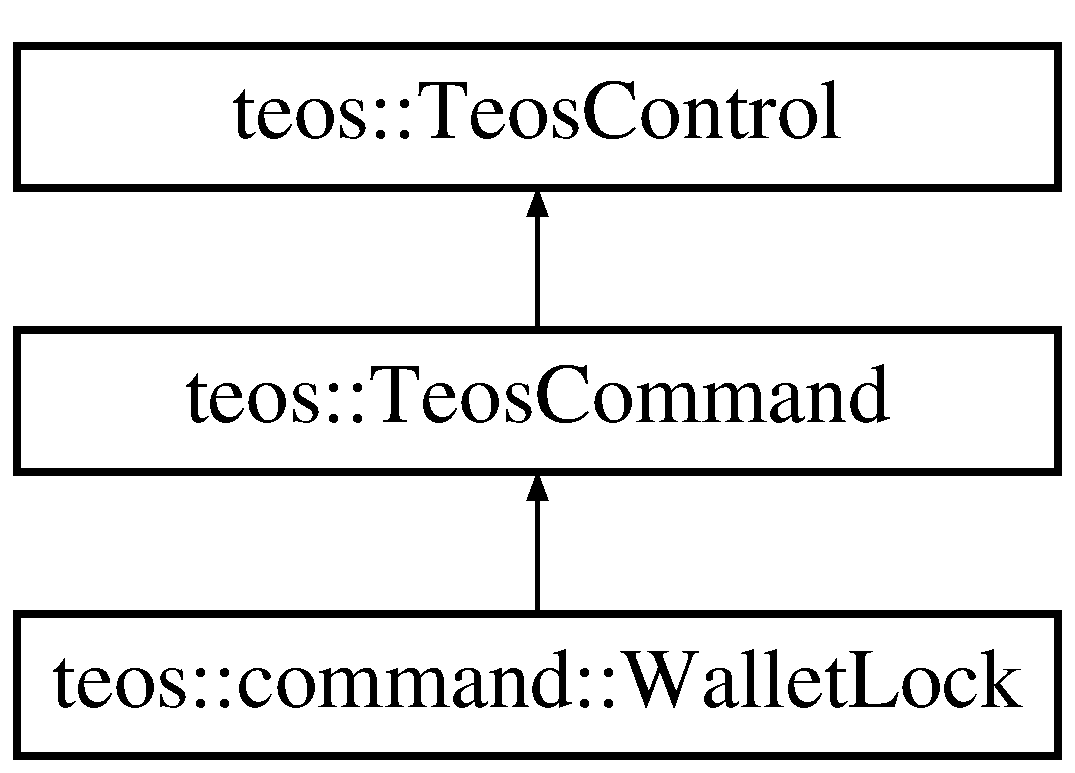
\includegraphics[height=3.000000cm]{classteos_1_1command_1_1_wallet_lock}
\end{center}
\end{figure}
\subsection*{Public Member Functions}
\begin{DoxyCompactItemize}
\item 
\mbox{\Hypertarget{classteos_1_1command_1_1_wallet_lock_a5e80a3195774c7911d716ff4fa41a4e7}\label{classteos_1_1command_1_1_wallet_lock_a5e80a3195774c7911d716ff4fa41a4e7}} 
{\bfseries Wallet\+Lock} (string name=D\+E\+F\+A\+U\+L\+T\+\_\+\+W\+A\+L\+L\+E\+T\+\_\+\+N\+A\+ME)
\item 
\mbox{\Hypertarget{classteos_1_1command_1_1_wallet_lock_a37c8f6a1c32d651c2ef1f2aabfd9207d}\label{classteos_1_1command_1_1_wallet_lock_a37c8f6a1c32d651c2ef1f2aabfd9207d}} 
{\bfseries Wallet\+Lock} (ptree req\+Json)
\item 
\mbox{\Hypertarget{classteos_1_1command_1_1_wallet_lock_aa2f7dbb10a35e4817467f2b4b95a0b95}\label{classteos_1_1command_1_1_wallet_lock_aa2f7dbb10a35e4817467f2b4b95a0b95}} 
string {\bfseries norm\+Request} (ptree \&req\+Json)
\item 
\mbox{\Hypertarget{classteos_1_1command_1_1_wallet_lock_afa87feb8243bc8ccdaf3438ba4817a9d}\label{classteos_1_1command_1_1_wallet_lock_afa87feb8243bc8ccdaf3438ba4817a9d}} 
void {\bfseries norm\+Response} (string response, ptree \&resp\+Json)
\end{DoxyCompactItemize}
\subsection*{Additional Inherited Members}


\subsection{Detailed Description}
Lock wallet. 

The documentation for this class was generated from the following file\+:\begin{DoxyCompactItemize}
\item 
teos\+\_\+lib/include/teoslib/command/wallet\+\_\+commands.\+hpp\end{DoxyCompactItemize}

\hypertarget{classteos_1_1command_1_1_wallet_lock_all}{}\section{teos\+:\+:command\+:\+:Wallet\+Lock\+All Class Reference}
\label{classteos_1_1command_1_1_wallet_lock_all}\index{teos\+::command\+::\+Wallet\+Lock\+All@{teos\+::command\+::\+Wallet\+Lock\+All}}


Lock all unlocked wallets.  




{\ttfamily \#include $<$wallet\+\_\+commands.\+hpp$>$}

Inheritance diagram for teos\+:\+:command\+:\+:Wallet\+Lock\+All\+:\begin{figure}[H]
\begin{center}
\leavevmode
\includegraphics[height=3.000000cm]{classteos_1_1command_1_1_wallet_lock_all}
\end{center}
\end{figure}
\subsection*{Public Member Functions}
\begin{DoxyCompactItemize}
\item 
\mbox{\Hypertarget{classteos_1_1command_1_1_wallet_lock_all_aaf4e6b212639281d2a5008a0ae798441}\label{classteos_1_1command_1_1_wallet_lock_all_aaf4e6b212639281d2a5008a0ae798441}} 
{\bfseries Wallet\+Lock\+All} (ptree req\+Json)
\item 
\mbox{\Hypertarget{classteos_1_1command_1_1_wallet_lock_all_a03ad4d17f33bec997d3c4d6ff67ea92a}\label{classteos_1_1command_1_1_wallet_lock_all_a03ad4d17f33bec997d3c4d6ff67ea92a}} 
string {\bfseries norm\+Request} (ptree \&req\+Json)
\item 
\mbox{\Hypertarget{classteos_1_1command_1_1_wallet_lock_all_abc6a2eb5f15f0f2e95b34ceb3f12339e}\label{classteos_1_1command_1_1_wallet_lock_all_abc6a2eb5f15f0f2e95b34ceb3f12339e}} 
void {\bfseries norm\+Response} (string response, ptree \&resp\+Json)
\end{DoxyCompactItemize}
\subsection*{Additional Inherited Members}


\subsection{Detailed Description}
Lock all unlocked wallets. 

The documentation for this class was generated from the following file\+:\begin{DoxyCompactItemize}
\item 
teos\+\_\+lib/include/teoslib/command/wallet\+\_\+commands.\+hpp\end{DoxyCompactItemize}

\hypertarget{classteos_1_1command_1_1_wallet_lock_all_options}{}\section{teos\+:\+:command\+:\+:Wallet\+Lock\+All\+Options Class Reference}
\label{classteos_1_1command_1_1_wallet_lock_all_options}\index{teos\+::command\+::\+Wallet\+Lock\+All\+Options@{teos\+::command\+::\+Wallet\+Lock\+All\+Options}}


Command-\/line driver for the \mbox{\hyperlink{classteos_1_1command_1_1_wallet_lock_all}{Wallet\+Lock\+All}} class.  




{\ttfamily \#include $<$wallet\+\_\+commands.\+hpp$>$}

Inheritance diagram for teos\+:\+:command\+:\+:Wallet\+Lock\+All\+Options\+:\begin{figure}[H]
\begin{center}
\leavevmode
\includegraphics[height=3.000000cm]{classteos_1_1command_1_1_wallet_lock_all_options}
\end{center}
\end{figure}
\subsection*{Public Member Functions}
\begin{DoxyCompactItemize}
\item 
\mbox{\Hypertarget{classteos_1_1command_1_1_wallet_lock_all_options_ac2aa30d7cdd0d8a0813e72b1773074b6}\label{classteos_1_1command_1_1_wallet_lock_all_options_ac2aa30d7cdd0d8a0813e72b1773074b6}} 
{\bfseries Wallet\+Lock\+All\+Options} (int argc, const char $\ast$$\ast$argv)
\end{DoxyCompactItemize}
\subsection*{Protected Member Functions}
\begin{DoxyCompactItemize}
\item 
const char $\ast$ \mbox{\hyperlink{classteos_1_1command_1_1_wallet_lock_all_options_ae45881c064f3d14883f3a1fae105603a}{get\+Usage}} ()
\begin{DoxyCompactList}\small\item\em Command \textquotesingle{}usage\textquotesingle{} instruction. \end{DoxyCompactList}\item 
\mbox{\Hypertarget{classteos_1_1command_1_1_wallet_lock_all_options_ac6ae053d93b6272aa142720cc9020c51}\label{classteos_1_1command_1_1_wallet_lock_all_options_ac6ae053d93b6272aa142720cc9020c51}} 
\mbox{\hyperlink{classteos_1_1_teos_control}{Teos\+Control}} {\bfseries execute\+Command} ()
\item 
\mbox{\Hypertarget{classteos_1_1command_1_1_wallet_lock_all_options_a787263cef86df3559a160bbe3c2507af}\label{classteos_1_1command_1_1_wallet_lock_all_options_a787263cef86df3559a160bbe3c2507af}} 
void {\bfseries printout} (\mbox{\hyperlink{classteos_1_1_teos_control}{Teos\+Control}} command, variables\+\_\+map \&vm)
\end{DoxyCompactItemize}
\subsection*{Additional Inherited Members}


\subsection{Detailed Description}
Command-\/line driver for the \mbox{\hyperlink{classteos_1_1command_1_1_wallet_lock_all}{Wallet\+Lock\+All}} class. 

\subsection{Member Function Documentation}
\mbox{\Hypertarget{classteos_1_1command_1_1_wallet_lock_all_options_ae45881c064f3d14883f3a1fae105603a}\label{classteos_1_1command_1_1_wallet_lock_all_options_ae45881c064f3d14883f3a1fae105603a}} 
\index{teos\+::command\+::\+Wallet\+Lock\+All\+Options@{teos\+::command\+::\+Wallet\+Lock\+All\+Options}!get\+Usage@{get\+Usage}}
\index{get\+Usage@{get\+Usage}!teos\+::command\+::\+Wallet\+Lock\+All\+Options@{teos\+::command\+::\+Wallet\+Lock\+All\+Options}}
\subsubsection{\texorpdfstring{get\+Usage()}{getUsage()}}
{\footnotesize\ttfamily const char$\ast$ teos\+::command\+::\+Wallet\+Lock\+All\+Options\+::get\+Usage (\begin{DoxyParamCaption}{ }\end{DoxyParamCaption})\hspace{0.3cm}{\ttfamily [inline]}, {\ttfamily [protected]}, {\ttfamily [virtual]}}



Command \textquotesingle{}usage\textquotesingle{} instruction. 

\begin{DoxyReturn}{Returns}
usage text 
\end{DoxyReturn}


Reimplemented from \mbox{\hyperlink{classteos_1_1_control_options_a0aa5671f9bc750ed5280c26c543874f3}{teos\+::\+Control\+Options}}.



The documentation for this class was generated from the following file\+:\begin{DoxyCompactItemize}
\item 
include/teoslib/command/wallet\+\_\+commands.\+hpp\end{DoxyCompactItemize}

\hypertarget{classteos_1_1command_1_1_wallet_lock_options}{}\section{teos\+:\+:command\+:\+:Wallet\+Lock\+Options Class Reference}
\label{classteos_1_1command_1_1_wallet_lock_options}\index{teos\+::command\+::\+Wallet\+Lock\+Options@{teos\+::command\+::\+Wallet\+Lock\+Options}}


Command-\/line driver for the \mbox{\hyperlink{classteos_1_1command_1_1_wallet_list}{Wallet\+List}} class.  




{\ttfamily \#include $<$wallet\+\_\+commands.\+hpp$>$}

Inheritance diagram for teos\+:\+:command\+:\+:Wallet\+Lock\+Options\+:\begin{figure}[H]
\begin{center}
\leavevmode
\includegraphics[height=3.000000cm]{classteos_1_1command_1_1_wallet_lock_options}
\end{center}
\end{figure}
\subsection*{Public Member Functions}
\begin{DoxyCompactItemize}
\item 
\mbox{\Hypertarget{classteos_1_1command_1_1_wallet_lock_options_ad486e3cb96e7061b85f5154e0595c725}\label{classteos_1_1command_1_1_wallet_lock_options_ad486e3cb96e7061b85f5154e0595c725}} 
{\bfseries Wallet\+Lock\+Options} (int argc, const char $\ast$$\ast$argv)
\end{DoxyCompactItemize}
\subsection*{Protected Member Functions}
\begin{DoxyCompactItemize}
\item 
const char $\ast$ \mbox{\hyperlink{classteos_1_1command_1_1_wallet_lock_options_aa0b3fd6dc244e1f32955c7a134b4fd85}{get\+Usage}} ()
\begin{DoxyCompactList}\small\item\em Command \textquotesingle{}usage\textquotesingle{} instruction. \end{DoxyCompactList}\item 
\mbox{\Hypertarget{classteos_1_1command_1_1_wallet_lock_options_ada29e51e9d79f51b13978af31167ef54}\label{classteos_1_1command_1_1_wallet_lock_options_ada29e51e9d79f51b13978af31167ef54}} 
options\+\_\+description {\bfseries argument\+Description} ()
\item 
\mbox{\Hypertarget{classteos_1_1command_1_1_wallet_lock_options_ae7e05a92f3382c85a3852d91958eb4d4}\label{classteos_1_1command_1_1_wallet_lock_options_ae7e05a92f3382c85a3852d91958eb4d4}} 
void {\bfseries set\+Pos\+Desc} (positional\+\_\+options\+\_\+description \&pos\+\_\+desc)
\item 
\mbox{\Hypertarget{classteos_1_1command_1_1_wallet_lock_options_ad0346ac84f5d101eb1afe82c5b376476}\label{classteos_1_1command_1_1_wallet_lock_options_ad0346ac84f5d101eb1afe82c5b376476}} 
bool {\bfseries check\+Arguments} (variables\+\_\+map \&vm)
\item 
\mbox{\Hypertarget{classteos_1_1command_1_1_wallet_lock_options_a70a5af011af56d22bf6c7dea6670e516}\label{classteos_1_1command_1_1_wallet_lock_options_a70a5af011af56d22bf6c7dea6670e516}} 
\mbox{\hyperlink{classteos_1_1_teos_control}{Teos\+Control}} {\bfseries execute\+Command} ()
\item 
\mbox{\Hypertarget{classteos_1_1command_1_1_wallet_lock_options_a9838bc30c785c2ff6312eada29f9d166}\label{classteos_1_1command_1_1_wallet_lock_options_a9838bc30c785c2ff6312eada29f9d166}} 
void {\bfseries printout} (\mbox{\hyperlink{classteos_1_1_teos_control}{Teos\+Control}} command, variables\+\_\+map \&vm)
\end{DoxyCompactItemize}
\subsection*{Protected Attributes}
\begin{DoxyCompactItemize}
\item 
\mbox{\Hypertarget{classteos_1_1command_1_1_wallet_lock_options_a17d6946277cea8daeeb11395a88ac84c}\label{classteos_1_1command_1_1_wallet_lock_options_a17d6946277cea8daeeb11395a88ac84c}} 
string {\bfseries name}
\end{DoxyCompactItemize}
\subsection*{Additional Inherited Members}


\subsection{Detailed Description}
Command-\/line driver for the \mbox{\hyperlink{classteos_1_1command_1_1_wallet_list}{Wallet\+List}} class. 

\subsection{Member Function Documentation}
\mbox{\Hypertarget{classteos_1_1command_1_1_wallet_lock_options_aa0b3fd6dc244e1f32955c7a134b4fd85}\label{classteos_1_1command_1_1_wallet_lock_options_aa0b3fd6dc244e1f32955c7a134b4fd85}} 
\index{teos\+::command\+::\+Wallet\+Lock\+Options@{teos\+::command\+::\+Wallet\+Lock\+Options}!get\+Usage@{get\+Usage}}
\index{get\+Usage@{get\+Usage}!teos\+::command\+::\+Wallet\+Lock\+Options@{teos\+::command\+::\+Wallet\+Lock\+Options}}
\subsubsection{\texorpdfstring{get\+Usage()}{getUsage()}}
{\footnotesize\ttfamily const char$\ast$ teos\+::command\+::\+Wallet\+Lock\+Options\+::get\+Usage (\begin{DoxyParamCaption}{ }\end{DoxyParamCaption})\hspace{0.3cm}{\ttfamily [inline]}, {\ttfamily [protected]}, {\ttfamily [virtual]}}



Command \textquotesingle{}usage\textquotesingle{} instruction. 

\begin{DoxyReturn}{Returns}
usage text 
\end{DoxyReturn}


Reimplemented from \mbox{\hyperlink{classteos_1_1_control_options_a0aa5671f9bc750ed5280c26c543874f3}{teos\+::\+Control\+Options}}.



The documentation for this class was generated from the following file\+:\begin{DoxyCompactItemize}
\item 
include/teoslib/command/wallet\+\_\+commands.\+hpp\end{DoxyCompactItemize}

\hypertarget{classteos_1_1command_1_1_wallet_open}{}\section{teos\+:\+:command\+:\+:Wallet\+Open Class Reference}
\label{classteos_1_1command_1_1_wallet_open}\index{teos\+::command\+::\+Wallet\+Open@{teos\+::command\+::\+Wallet\+Open}}


Open an existing wallet.  




{\ttfamily \#include $<$wallet\+\_\+commands.\+hpp$>$}

Inheritance diagram for teos\+:\+:command\+:\+:Wallet\+Open\+:\begin{figure}[H]
\begin{center}
\leavevmode
\includegraphics[height=3.000000cm]{classteos_1_1command_1_1_wallet_open}
\end{center}
\end{figure}
\subsection*{Public Member Functions}
\begin{DoxyCompactItemize}
\item 
\mbox{\Hypertarget{classteos_1_1command_1_1_wallet_open_a83737d8d2e5f335266e331e3771c50b4}\label{classteos_1_1command_1_1_wallet_open_a83737d8d2e5f335266e331e3771c50b4}} 
{\bfseries Wallet\+Open} (string name=D\+E\+F\+A\+U\+L\+T\+\_\+\+W\+A\+L\+L\+E\+T\+\_\+\+N\+A\+ME)
\item 
\mbox{\Hypertarget{classteos_1_1command_1_1_wallet_open_afe4f67f6e891bf5dcc4e5fb02e372e3f}\label{classteos_1_1command_1_1_wallet_open_afe4f67f6e891bf5dcc4e5fb02e372e3f}} 
{\bfseries Wallet\+Open} (ptree req\+Json)
\item 
\mbox{\Hypertarget{classteos_1_1command_1_1_wallet_open_a7de38b779a421c4964af4679dc5d24f7}\label{classteos_1_1command_1_1_wallet_open_a7de38b779a421c4964af4679dc5d24f7}} 
string {\bfseries norm\+Request} (ptree \&req\+Json)
\item 
\mbox{\Hypertarget{classteos_1_1command_1_1_wallet_open_aa8b15aa97a21e79224d627a7417f1bda}\label{classteos_1_1command_1_1_wallet_open_aa8b15aa97a21e79224d627a7417f1bda}} 
void {\bfseries norm\+Response} (string response, ptree \&resp\+Json)
\end{DoxyCompactItemize}
\subsection*{Additional Inherited Members}


\subsection{Detailed Description}
Open an existing wallet. 

The documentation for this class was generated from the following file\+:\begin{DoxyCompactItemize}
\item 
teos\+\_\+lib/include/teoslib/command/wallet\+\_\+commands.\+hpp\end{DoxyCompactItemize}

\hypertarget{classteos_1_1command_1_1_wallet_open_options}{}\section{teos\+:\+:command\+:\+:Wallet\+Open\+Options Class Reference}
\label{classteos_1_1command_1_1_wallet_open_options}\index{teos\+::command\+::\+Wallet\+Open\+Options@{teos\+::command\+::\+Wallet\+Open\+Options}}
Inheritance diagram for teos\+:\+:command\+:\+:Wallet\+Open\+Options\+:\begin{figure}[H]
\begin{center}
\leavevmode
\includegraphics[height=3.000000cm]{classteos_1_1command_1_1_wallet_open_options}
\end{center}
\end{figure}
\subsection*{Public Member Functions}
\begin{DoxyCompactItemize}
\item 
\mbox{\Hypertarget{classteos_1_1command_1_1_wallet_open_options_acca0aca60a4dfb23f0a87cbb551ed473}\label{classteos_1_1command_1_1_wallet_open_options_acca0aca60a4dfb23f0a87cbb551ed473}} 
{\bfseries Wallet\+Open\+Options} (int argc, const char $\ast$$\ast$argv)
\end{DoxyCompactItemize}
\subsection*{Protected Member Functions}
\begin{DoxyCompactItemize}
\item 
const char $\ast$ \mbox{\hyperlink{classteos_1_1command_1_1_wallet_open_options_aedf25a6f772392c2cb0c0de8d80172dd}{get\+Usage}} ()
\begin{DoxyCompactList}\small\item\em Command \textquotesingle{}usage\textquotesingle{} instruction. \end{DoxyCompactList}\item 
\mbox{\Hypertarget{classteos_1_1command_1_1_wallet_open_options_ad23269217ec4accc93b3d9ba04c5db47}\label{classteos_1_1command_1_1_wallet_open_options_ad23269217ec4accc93b3d9ba04c5db47}} 
options\+\_\+description {\bfseries argument\+Description} ()
\item 
\mbox{\Hypertarget{classteos_1_1command_1_1_wallet_open_options_ae01566fb06b790e8b2783c4c302ce06f}\label{classteos_1_1command_1_1_wallet_open_options_ae01566fb06b790e8b2783c4c302ce06f}} 
void {\bfseries set\+Pos\+Desc} (positional\+\_\+options\+\_\+description \&pos\+\_\+desc)
\item 
\mbox{\Hypertarget{classteos_1_1command_1_1_wallet_open_options_a68617d7ca15de92006db594521c710de}\label{classteos_1_1command_1_1_wallet_open_options_a68617d7ca15de92006db594521c710de}} 
bool {\bfseries check\+Arguments} (variables\+\_\+map \&vm)
\item 
\mbox{\Hypertarget{classteos_1_1command_1_1_wallet_open_options_a4aec1942f5a46b8565a9ca4e97d6cdf0}\label{classteos_1_1command_1_1_wallet_open_options_a4aec1942f5a46b8565a9ca4e97d6cdf0}} 
\mbox{\hyperlink{classteos_1_1_teos_control}{Teos\+Control}} {\bfseries execute\+Command} ()
\item 
\mbox{\Hypertarget{classteos_1_1command_1_1_wallet_open_options_a580c7a2b14967ae71abe570515685269}\label{classteos_1_1command_1_1_wallet_open_options_a580c7a2b14967ae71abe570515685269}} 
void {\bfseries printout} (\mbox{\hyperlink{classteos_1_1_teos_control}{Teos\+Control}} command, variables\+\_\+map \&vm)
\end{DoxyCompactItemize}
\subsection*{Protected Attributes}
\begin{DoxyCompactItemize}
\item 
\mbox{\Hypertarget{classteos_1_1command_1_1_wallet_open_options_a3a8ee8998dfdff2290165e6eb5403291}\label{classteos_1_1command_1_1_wallet_open_options_a3a8ee8998dfdff2290165e6eb5403291}} 
string {\bfseries name}
\end{DoxyCompactItemize}
\subsection*{Additional Inherited Members}


\subsection{Member Function Documentation}
\mbox{\Hypertarget{classteos_1_1command_1_1_wallet_open_options_aedf25a6f772392c2cb0c0de8d80172dd}\label{classteos_1_1command_1_1_wallet_open_options_aedf25a6f772392c2cb0c0de8d80172dd}} 
\index{teos\+::command\+::\+Wallet\+Open\+Options@{teos\+::command\+::\+Wallet\+Open\+Options}!get\+Usage@{get\+Usage}}
\index{get\+Usage@{get\+Usage}!teos\+::command\+::\+Wallet\+Open\+Options@{teos\+::command\+::\+Wallet\+Open\+Options}}
\subsubsection{\texorpdfstring{get\+Usage()}{getUsage()}}
{\footnotesize\ttfamily const char$\ast$ teos\+::command\+::\+Wallet\+Open\+Options\+::get\+Usage (\begin{DoxyParamCaption}{ }\end{DoxyParamCaption})\hspace{0.3cm}{\ttfamily [inline]}, {\ttfamily [protected]}, {\ttfamily [virtual]}}



Command \textquotesingle{}usage\textquotesingle{} instruction. 

\begin{DoxyReturn}{Returns}
usage text 
\end{DoxyReturn}


Reimplemented from \mbox{\hyperlink{classteos_1_1_control_options_a0aa5671f9bc750ed5280c26c543874f3}{teos\+::\+Control\+Options}}.



The documentation for this class was generated from the following file\+:\begin{DoxyCompactItemize}
\item 
teos\+\_\+lib/include/teoslib/command/wallet\+\_\+commands.\+hpp\end{DoxyCompactItemize}

\hypertarget{classteos_1_1command_1_1_wallet_unlock}{}\section{teos\+:\+:command\+:\+:Wallet\+Unlock Class Reference}
\label{classteos_1_1command_1_1_wallet_unlock}\index{teos\+::command\+::\+Wallet\+Unlock@{teos\+::command\+::\+Wallet\+Unlock}}


Unlock wallet.  




{\ttfamily \#include $<$wallet\+\_\+commands.\+hpp$>$}

Inheritance diagram for teos\+:\+:command\+:\+:Wallet\+Unlock\+:\begin{figure}[H]
\begin{center}
\leavevmode
\includegraphics[height=3.000000cm]{classteos_1_1command_1_1_wallet_unlock}
\end{center}
\end{figure}
\subsection*{Public Member Functions}
\begin{DoxyCompactItemize}
\item 
\mbox{\Hypertarget{classteos_1_1command_1_1_wallet_unlock_a87eecaca05f1c7c96dda5de7c1b35c0e}\label{classteos_1_1command_1_1_wallet_unlock_a87eecaca05f1c7c96dda5de7c1b35c0e}} 
{\bfseries Wallet\+Unlock} (string password, string name=D\+E\+F\+A\+U\+L\+T\+\_\+\+W\+A\+L\+L\+E\+T\+\_\+\+N\+A\+ME)
\item 
\mbox{\Hypertarget{classteos_1_1command_1_1_wallet_unlock_a8f5f39f30a96a1c176f2fb5249bdfa0b}\label{classteos_1_1command_1_1_wallet_unlock_a8f5f39f30a96a1c176f2fb5249bdfa0b}} 
{\bfseries Wallet\+Unlock} (ptree req\+Json)
\item 
\mbox{\Hypertarget{classteos_1_1command_1_1_wallet_unlock_a186153f624725bddb198992c7ffde702}\label{classteos_1_1command_1_1_wallet_unlock_a186153f624725bddb198992c7ffde702}} 
string {\bfseries norm\+Request} (ptree \&req\+Json)
\item 
\mbox{\Hypertarget{classteos_1_1command_1_1_wallet_unlock_ad8eb4d249f3305fa9beb3b69280e889d}\label{classteos_1_1command_1_1_wallet_unlock_ad8eb4d249f3305fa9beb3b69280e889d}} 
void {\bfseries norm\+Response} (string response, ptree \&resp\+Json)
\end{DoxyCompactItemize}
\subsection*{Additional Inherited Members}


\subsection{Detailed Description}
Unlock wallet. 

The documentation for this class was generated from the following file\+:\begin{DoxyCompactItemize}
\item 
teos\+\_\+lib/include/teoslib/command/wallet\+\_\+commands.\+hpp\end{DoxyCompactItemize}

\hypertarget{classteos_1_1command_1_1_wallet_unlock_options}{}\section{teos\+:\+:command\+:\+:Wallet\+Unlock\+Options Class Reference}
\label{classteos_1_1command_1_1_wallet_unlock_options}\index{teos\+::command\+::\+Wallet\+Unlock\+Options@{teos\+::command\+::\+Wallet\+Unlock\+Options}}


Command-\/line driver for the \mbox{\hyperlink{classteos_1_1command_1_1_wallet_unlock}{Wallet\+Unlock}} class.  




{\ttfamily \#include $<$wallet\+\_\+commands.\+hpp$>$}

Inheritance diagram for teos\+:\+:command\+:\+:Wallet\+Unlock\+Options\+:\begin{figure}[H]
\begin{center}
\leavevmode
\includegraphics[height=3.000000cm]{classteos_1_1command_1_1_wallet_unlock_options}
\end{center}
\end{figure}
\subsection*{Public Member Functions}
\begin{DoxyCompactItemize}
\item 
\mbox{\Hypertarget{classteos_1_1command_1_1_wallet_unlock_options_a2b5254389e6bac32bd88a30ee6f92d78}\label{classteos_1_1command_1_1_wallet_unlock_options_a2b5254389e6bac32bd88a30ee6f92d78}} 
{\bfseries Wallet\+Unlock\+Options} (int argc, const char $\ast$$\ast$argv)
\end{DoxyCompactItemize}
\subsection*{Protected Member Functions}
\begin{DoxyCompactItemize}
\item 
const char $\ast$ \mbox{\hyperlink{classteos_1_1command_1_1_wallet_unlock_options_aa630c4deec62ef8d44cb37c03573c071}{get\+Usage}} ()
\begin{DoxyCompactList}\small\item\em Command \textquotesingle{}usage\textquotesingle{} instruction. \end{DoxyCompactList}\item 
\mbox{\Hypertarget{classteos_1_1command_1_1_wallet_unlock_options_a668aae33dff94bcc5fe964cfd5712666}\label{classteos_1_1command_1_1_wallet_unlock_options_a668aae33dff94bcc5fe964cfd5712666}} 
options\+\_\+description {\bfseries argument\+Description} ()
\item 
\mbox{\Hypertarget{classteos_1_1command_1_1_wallet_unlock_options_a7650a6cb1eb82ab04334561b5792b736}\label{classteos_1_1command_1_1_wallet_unlock_options_a7650a6cb1eb82ab04334561b5792b736}} 
void {\bfseries set\+Pos\+Desc} (positional\+\_\+options\+\_\+description \&pos\+\_\+desc)
\item 
\mbox{\Hypertarget{classteos_1_1command_1_1_wallet_unlock_options_a3c8982dfec1c8affd25a7cb389388afb}\label{classteos_1_1command_1_1_wallet_unlock_options_a3c8982dfec1c8affd25a7cb389388afb}} 
bool {\bfseries check\+Arguments} (variables\+\_\+map \&vm)
\item 
\mbox{\Hypertarget{classteos_1_1command_1_1_wallet_unlock_options_a97a2d0020caa85625bb2611203468367}\label{classteos_1_1command_1_1_wallet_unlock_options_a97a2d0020caa85625bb2611203468367}} 
\mbox{\hyperlink{classteos_1_1_teos_control}{Teos\+Control}} {\bfseries execute\+Command} ()
\item 
\mbox{\Hypertarget{classteos_1_1command_1_1_wallet_unlock_options_acc359227ff0f0962753c5b1ffc264ae8}\label{classteos_1_1command_1_1_wallet_unlock_options_acc359227ff0f0962753c5b1ffc264ae8}} 
void {\bfseries printout} (\mbox{\hyperlink{classteos_1_1_teos_control}{Teos\+Control}} command, variables\+\_\+map \&vm)
\end{DoxyCompactItemize}
\subsection*{Protected Attributes}
\begin{DoxyCompactItemize}
\item 
\mbox{\Hypertarget{classteos_1_1command_1_1_wallet_unlock_options_a28631c65fbc2cf6f3ce740329fad87a4}\label{classteos_1_1command_1_1_wallet_unlock_options_a28631c65fbc2cf6f3ce740329fad87a4}} 
string {\bfseries name}
\item 
\mbox{\Hypertarget{classteos_1_1command_1_1_wallet_unlock_options_a189cfcbe96d25146d7002ff5b8405485}\label{classteos_1_1command_1_1_wallet_unlock_options_a189cfcbe96d25146d7002ff5b8405485}} 
string {\bfseries password}
\end{DoxyCompactItemize}
\subsection*{Additional Inherited Members}


\subsection{Detailed Description}
Command-\/line driver for the \mbox{\hyperlink{classteos_1_1command_1_1_wallet_unlock}{Wallet\+Unlock}} class. 

\subsection{Member Function Documentation}
\mbox{\Hypertarget{classteos_1_1command_1_1_wallet_unlock_options_aa630c4deec62ef8d44cb37c03573c071}\label{classteos_1_1command_1_1_wallet_unlock_options_aa630c4deec62ef8d44cb37c03573c071}} 
\index{teos\+::command\+::\+Wallet\+Unlock\+Options@{teos\+::command\+::\+Wallet\+Unlock\+Options}!get\+Usage@{get\+Usage}}
\index{get\+Usage@{get\+Usage}!teos\+::command\+::\+Wallet\+Unlock\+Options@{teos\+::command\+::\+Wallet\+Unlock\+Options}}
\subsubsection{\texorpdfstring{get\+Usage()}{getUsage()}}
{\footnotesize\ttfamily const char$\ast$ teos\+::command\+::\+Wallet\+Unlock\+Options\+::get\+Usage (\begin{DoxyParamCaption}{ }\end{DoxyParamCaption})\hspace{0.3cm}{\ttfamily [inline]}, {\ttfamily [protected]}, {\ttfamily [virtual]}}



Command \textquotesingle{}usage\textquotesingle{} instruction. 

\begin{DoxyReturn}{Returns}
usage text 
\end{DoxyReturn}


Reimplemented from \mbox{\hyperlink{classteos_1_1_control_options_a0aa5671f9bc750ed5280c26c543874f3}{teos\+::\+Control\+Options}}.



The documentation for this class was generated from the following file\+:\begin{DoxyCompactItemize}
\item 
teos\+\_\+lib/include/teoslib/command/wallet\+\_\+commands.\+hpp\end{DoxyCompactItemize}

\chapter{File Documentation}
\hypertarget{command_8hpp}{}\section{teos\+\_\+lib/include/teoslib/command.hpp File Reference}
\label{command_8hpp}\index{teos\+\_\+lib/include/teoslib/command.\+hpp@{teos\+\_\+lib/include/teoslib/command.\+hpp}}


Tool for sending transactions and querying state from E\+OS blockchain.  


{\ttfamily \#include $<$teoslib/control.\+hpp$>$}\newline
{\ttfamily \#include $<$teoslib/control/config.\+hpp$>$}\newline
\subsection*{Classes}
\begin{DoxyCompactItemize}
\item 
class \mbox{\hyperlink{classteos_1_1_teos_command}{teos\+::\+Teos\+Command}}
\item 
class \mbox{\hyperlink{classteos_1_1_command_options}{teos\+::\+Command\+Options}}
\end{DoxyCompactItemize}
\subsection*{Macros}
\begin{DoxyCompactItemize}
\item 
\mbox{\Hypertarget{command_8hpp_aba176152ccdd4a378174a5de6dfd28c3}\label{command_8hpp_aba176152ccdd4a378174a5de6dfd28c3}} 
\#define {\bfseries T\+O\+K\+E\+N\+I\+K\+A\+\_\+\+W\+A\+L\+L\+ET}~\char`\"{}tokenika\+Wallet\char`\"{}
\end{DoxyCompactItemize}
\subsection*{Variables}
\begin{DoxyCompactItemize}
\item 
\mbox{\Hypertarget{command_8hpp_ae9a7c17dc3f1916a3e37ac1968874850}\label{command_8hpp_ae9a7c17dc3f1916a3e37ac1968874850}} 
const string {\bfseries wallet\+Command\+Path}
\end{DoxyCompactItemize}


\subsection{Detailed Description}
Tool for sending transactions and querying state from E\+OS blockchain. 

\begin{DoxyCopyright}{Copyright}
defined in resources/\+L\+I\+C\+E\+N\+S\+E.\+txt Base definitions.
\end{DoxyCopyright}
Defines base classes of the project, and helper methods. 
\hypertarget{get__commands_8hpp}{}\section{teos\+\_\+lib/include/teoslib/command/get\+\_\+commands.hpp File Reference}
\label{get__commands_8hpp}\index{teos\+\_\+lib/include/teoslib/command/get\+\_\+commands.\+hpp@{teos\+\_\+lib/include/teoslib/command/get\+\_\+commands.\+hpp}}
{\ttfamily \#include $<$boost/date\+\_\+time/posix\+\_\+time/posix\+\_\+time.\+hpp$>$}\newline
{\ttfamily \#include $<$boost/property\+\_\+tree/ptree.\+hpp$>$}\newline
{\ttfamily \#include $<$teoslib/config.\+h$>$}\newline
{\ttfamily \#include $<$teoslib/command.\+hpp$>$}\newline
{\ttfamily \#include $<$teoslib/eos\+\_\+interface.\+hpp$>$}\newline
\subsection*{Classes}
\begin{DoxyCompactItemize}
\item 
class \mbox{\hyperlink{classteos_1_1command_1_1_get_info}{teos\+::command\+::\+Get\+Info}}
\begin{DoxyCompactList}\small\item\em Get current blockchain information. \end{DoxyCompactList}\item 
class \mbox{\hyperlink{classteos_1_1command_1_1_get_info_options}{teos\+::command\+::\+Get\+Info\+Options}}
\begin{DoxyCompactList}\small\item\em Command-\/line driver for the \mbox{\hyperlink{classteos_1_1command_1_1_get_info}{Get\+Info}} class. \end{DoxyCompactList}\item 
class \mbox{\hyperlink{classteos_1_1command_1_1_get_block}{teos\+::command\+::\+Get\+Block}}
\begin{DoxyCompactList}\small\item\em Retrieve a full block from a blockchain. \end{DoxyCompactList}\item 
class \mbox{\hyperlink{classteos_1_1command_1_1_get_block_options}{teos\+::command\+::\+Get\+Block\+Options}}
\begin{DoxyCompactList}\small\item\em Command-\/line driver for the \mbox{\hyperlink{classteos_1_1command_1_1_get_block}{Get\+Block}} class. \end{DoxyCompactList}\item 
class \mbox{\hyperlink{classteos_1_1command_1_1_get_account}{teos\+::command\+::\+Get\+Account}}
\begin{DoxyCompactList}\small\item\em Fetch a blockchain account. \end{DoxyCompactList}\item 
class \mbox{\hyperlink{classteos_1_1command_1_1_get_account_options}{teos\+::command\+::\+Get\+Account\+Options}}
\begin{DoxyCompactList}\small\item\em Command-\/line driver for the \mbox{\hyperlink{classteos_1_1command_1_1_get_account}{Get\+Account}} class. \end{DoxyCompactList}\item 
class \mbox{\hyperlink{classteos_1_1command_1_1_get_accounts}{teos\+::command\+::\+Get\+Accounts}}
\begin{DoxyCompactList}\small\item\em Retrieve accounts associated with a public key. \end{DoxyCompactList}\item 
class \mbox{\hyperlink{classteos_1_1command_1_1_get_accounts_options}{teos\+::command\+::\+Get\+Accounts\+Options}}
\begin{DoxyCompactList}\small\item\em Command-\/line driver for the \mbox{\hyperlink{classteos_1_1command_1_1_get_accounts}{Get\+Accounts}} class. \end{DoxyCompactList}\item 
class \mbox{\hyperlink{classteos_1_1command_1_1_get_code}{teos\+::command\+::\+Get\+Code}}
\begin{DoxyCompactList}\small\item\em Retrieves the code and A\+BI for an account. \end{DoxyCompactList}\item 
class \mbox{\hyperlink{classteos_1_1command_1_1_get_code_options}{teos\+::command\+::\+Get\+Code\+Options}}
\begin{DoxyCompactList}\small\item\em Command-\/line driver for the \mbox{\hyperlink{classteos_1_1command_1_1_get_code}{Get\+Code}} class. \end{DoxyCompactList}\item 
class \mbox{\hyperlink{classteos_1_1command_1_1_get_table}{teos\+::command\+::\+Get\+Table}}
\begin{DoxyCompactList}\small\item\em Retrieves the contents of a database table. \end{DoxyCompactList}\item 
class \mbox{\hyperlink{classteos_1_1command_1_1_get_table_options}{teos\+::command\+::\+Get\+Table\+Options}}
\end{DoxyCompactItemize}
\subsection*{Macros}
\begin{DoxyCompactItemize}
\item 
\mbox{\Hypertarget{get__commands_8hpp_a9ed5e42972ae378b3a13417901f88aac}\label{get__commands_8hpp_a9ed5e42972ae378b3a13417901f88aac}} 
\#define {\bfseries G\+E\+T\+\_\+\+A\+C\+C\+O\+U\+N\+T\+S\+\_\+\+P\+A\+TH}~\char`\"{}/v1/account\+\_\+history/get\+\_\+key\+\_\+accounts\char`\"{}
\item 
\mbox{\Hypertarget{get__commands_8hpp_a8945ebbf71654265a82ab999fc8170ca}\label{get__commands_8hpp_a8945ebbf71654265a82ab999fc8170ca}} 
\#define {\bfseries W\+R\+I\+T\+E\+\_\+\+T\+O\+\_\+\+S\+T\+D\+O\+UT}~\char`\"{}stdout\char`\"{}
\end{DoxyCompactItemize}
\subsection*{Variables}
\begin{DoxyCompactItemize}
\item 
\mbox{\Hypertarget{get__commands_8hpp_a7c4fd28d5ba0ccb35063b65319248d09}\label{get__commands_8hpp_a7c4fd28d5ba0ccb35063b65319248d09}} 
const char $\ast$ {\bfseries get\+Subcommands}
\item 
\mbox{\Hypertarget{get__commands_8hpp_ac9afba63daabfb4bbc161a184912a560}\label{get__commands_8hpp_ac9afba63daabfb4bbc161a184912a560}} 
const string {\bfseries get\+Command\+Path}
\end{DoxyCompactItemize}


\subsection{Detailed Description}
Definitions for get-\/type commands.

Defines command line options. 
%--- End generated contents ---

% Index
\backmatter
\newpage
\phantomsection
\clearemptydoublepage
\addcontentsline{toc}{chapter}{Index}
\printindex

\end{document}
